\documentclass[type=bachelor, fontset=fandol, seriftoc]{cquthesis}%

% 可用选项：
% type=[bachelor|master|doctor],      % 必选，毕业论文类型，以下项目不填时为默认
% liberalformat,                      % 可选，仅适用本科生，使用文学类论文标题格式，默认未打开
% proffesionalmaster=[true|false],    % 可选，仅适用研究生，是(true)否(false)专业硕士，默认为否
% printmode=[oneside|twoside|auto],	  % 可选，论文打印方式，默认采用auto按页数要求自动判定
% openany,|openright,                 % 可选，双面打印时每章的第一页仅右页开启，默认右页开启(openright)
% bilinguallist=[off|combined|apart], % 可选，图录表录等分别按双语题注混编(combined)，分开编录(apart)，默认关(off)
% blindtrail,                         % 可选，盲审模式，开启后封面姓名和致谢部分会隐藏，详情请参阅用户文档，默认关
% draft,                              % 写作期间可选，不渲染图片，关闭外围功能，加快预览速度，默认未开启

% 请在cquthesis.sty文件中定义其他会用到的宏包和自己的变量
% 这样可以防止main.tex太过臃肿。
\usepackage{cquthesis}
\usepackage{ctex}        % 中文支持
\usepackage{graphicx}    % 图片插入
\usepackage{float}       % 图表位置控制[htbp]
\usepackage{booktabs}   % 三线表
\usepackage{array}      % p列支持
\usepackage{makecell}   % 可选，支持单元格换行
\usepackage[section]{placeins}
\usepackage{longtable}
\usepackage{multirow}

\usepackage{caption}
\captionsetup{
    font={small},         % 使用small字体（对应五号）
    labelsep=quad,        % 编号和标题之间空一个汉字符
    justification=centering % 标题居中
}
\captionsetup[table]{position=top,belowskip=6bp,aboveskip=0bp}
\captionsetup[figure]{position=bottom,belowskip=0bp,aboveskip=6bp}

% 2. 重新定义表格内的默认字体大小（2024模版要求：小五或small）
\makeatletter
\def\cqu@tabular{\small\@tabular}
\makeatother

% 3. 调整表格行高（如果觉得当前行高过大，可以适当调小）
\renewcommand{\arraystretch}{1.2} % 1.2到1.5之间视情况调整

% 定义所有的图片文件在 figures 子目录下
\graphicspath{{figures/}}





%*** 写作时，使用这个命令只渲染你想查看的部分，提升工作效率，定稿时注释掉整行
% \includeonly{contents/ch3_inflatable}
\begin{document}

\cqusetup{
  ctitle = {基于嵌入式机器人系统的车载 Agent\\——飞行雨伞的设计与实现},
  etitle = {Vehicle-Borne Agent Based on Embedded Robot System\\---Design and Implementation of Flying Umbrella},
  cauthor = {王浚西},
  eauthor = {Wang~Junxi},
  studentid = {20222660},
  csupervisor = {罗远新},
  esupervisor = {{Prof. Luo Yuanxin}},
  cassistsupervisor = {},
  cextrasupervisor = {},
  eassistsupervisor = {},
  cmajor = {机器人工程},
  emajor = {Robotics Engineering},
  cdepartment = {国家卓越工程师学院},
  edepartment = {National Elite Institute of Engineering, Chongqing University},
  mycdate = {2026年6月},
  myedate = {June, 2026},
}
% ===================
%
% 论文的摘要
%
% ===================
\begin{cabstract}
随着新能源汽车向着智能化方向发展，车载系统功能的边界也在发生变化，它的服务对象也由原来的车内扩展到了车外的实际使用场景。本文主要针对传统雨伞在出行时需要手持、会占用双手的问题，设计并实现了以充气结构为支撑的车载多形态飞行机器人系统——飞行雨伞。该系统把车辆当作地面部署的基准点，在收纳态和飞行遮蔽态之间实施主动形态调整，其主要目的就是给用户在下车遇雨的时候，赋予一种“随车常备、快速部署、双手解放”的遮雨手段。简单来说，它并不是把雨伞搬到飞行器上，而是试图把遮雨这件事情变成一种可以部署的车载服务能力。

本文采用无刚性承力件的充气模块化骨架结构。系统用标准快递气柱、PLA 3D打印节点构成正方形平面桁架骨架，再加TPU薄膜伞面形成遮蔽区域，得到一个$0.608\,\text{m}^2$的遮蔽面积。这样处理有一个非常直接的好处就是可以提供较大的遮蔽范围，排气之后又能整体压缩收纳，方便放在车载空间里。大面积遮蔽和紧凑收纳两个经常难以兼顾的要求，在本方案中得到了比较好的平衡。

在动力系统方面，针对整机实测起飞质量 $1683\,\text{g}$，本文选用 SIRIUS 2306.5-1850KV 电机与 51366 桨叶，并采用系留供电与机载电池互补的双模式供电方案。前者主要是做长时悬停，后者是应急备用或者紧急情况下独立工作的备用电源。该种设计思路比较务实，一方面考虑了持续供能，另一方面也保留了基本的机动和安全冗余，不至于使系统完全依靠单一的供电方式。

系统用Pixhawk6C开源飞控和PX4固件来搭建。由于充气伞体带来超大转动惯量、气动阻力比常规四旋翼要大得多，因此飞行器的控制特性与常见的四旋翼相比有很大不同。计算结果表明，其转动惯量约为同质量标准四旋翼的 17 倍，其中 $I_{xx}\approx0.210\,\text{kg}\cdot\text{m}^2$。如果直接使用默认的控制参数，系统在调试初期很容易产生较强的振荡。因此本文提出把比例增益设为默认值1/3的PID初始整定方法，使第一轮调参先控制在可控范围内，再进行更详细的优化。这一步看上去只是参数的缩放，但它对于系统顺利起飞、稳定悬停来说却至关重要。

从实验结果可以看出，充气骨架可以保持工作气压大于30min，有基本的使用稳定性；完整的工作流程中起飞准备时间是85s，排气收纳时间是48s，说明系统部署和回收过程比较紧凑。在姿态稳定模式下，飞行器实现了 Roll 轴 $\pm2.1^\circ$、Pitch 轴 $\pm1.8^\circ$ 的稳定悬停；在系留模式下，实测续航达到 18.2\,min。从整体上看各项指标都达到了预期的设计目的，说明系统方案具有较好的可实现性。

本文工作证明了充气结构对飞行器形态主动重构技术的可行性和可靠性，也为车载飞行机器人在个人出行场景下的工程化应用提供了一些经验。因此本研究不单考虑了“能否飞行”的问题，也考虑了“能否收运”、“能否携带”以及“能否真正服务于实际的出行场景”。
\end{cabstract}

\ckeywords{多旋翼飞行器,充气结构,形态重构,车载服务系统,PID控制}

\begin{eabstract}
In the context of the continuous intelligent development of new energy vehicles, the function boundary of the onboard system is being reformed, and its service capability is gradually expanding from the car interior to various other applications. The main topic of this thesis will be the inconvenience of traditional umbrellas; they need to be held with one hand, so it is not convenient to use both hands for other activities during travel, and therefore a vehicle-mounted multi-form aerial robotic system based on an inflatable structure called a "Flying Umbrella" will be put forward. The vehicle is to be used as the ground base of the system, and it can switch between a stowed state and a flying shelter mode. The main reason for this is that it is a rain-shielding device, can be carried in the car, is easy to deploy, and will not obstruct the user's hands. In short, it is not enough to have an umbrella for the flying platform; one should be installed on board the aircraft.
The shape of an inflatable skeleton structure will not be fixed and will have no supports. A square-plan truss has been made of standard express air columns and PLA 3D-printed joints, and a TPU film canopy will be added to form a shielding surface; it has reached an effective covered area of 0.608 m$^2$. The advantage of the above method is its relatively simple structure; after setting up the shelter, there will be a relatively large enclosed area, and after inflation, the whole structure can be folded for transport in a car. In short, the two Design Goals must be achieved at the same time, but they are often conflicting; that is to say, to increase the coverage area, more storage space is required.
Given that the measured take-off mass is $1683\,\text{g}$, SIRIUS 2306.5-1850KV motors and 51366 propellers will be chosen for the propulsion system, and a dual-mode power supply consisting of tethered power and an onboard battery will be used. The former is mainly for extended hovering; the latter is to be used in case of emergency and has a short service life. It is a reasonable plan that will extend the time people can exercise and keep them healthy and safe to some extent.
Pixhawk~6C is used as the open-source flight controller and PX4 is the firmware for flight control. Because of the relatively large moment of inertia and larger aerodynamic drag of the inflatable canopy, it will not be controlled in the same way as a typical quadrotor. The calculated inertia is about 17 times that of a standard quadrotor with the same mass, and $I_{xx} \approx 0.210\,\text{kg}\cdot\text{m}^2$. If the default controller parameters are used directly, there will be serious oscillation in the early stage of tuning. Therefore, the first PID tuning strategy is to reduce the proportional gain by one-third of the default value; thus, the first round of tuning can be in a stable state before further adjustment. The modification is relatively simple, but it will help the aircraft take off and hover stably.
As shown in the experiment above, the expanded skeleton can maintain the working pressure for more than 30 minutes and have some basic service stability. In the full operating procedure, the takeoff preparation time is 85 s and the deflation-and-stowage time is 48 s; therefore, both deployment and recovery can be carried out in a short amount of time. The attitude-stabilised mode can maintain the stability of the vehicle in flight, and the roll-axis deviation is $\le \pm 2.1^\circ$ and the pitch-axis deviation is $\le \pm 1.8^\circ$. The lifetime of Tethered Mode is 18.2 minutes. All of the main indicators have reached the goals set out in the design; thus, the system will be realised.
Based on the above research, it has been found that inflatable structures can be used to achieve the active deformation and reorganization of aerial vehicles, and some practical engineering experience has also been obtained for vehicle-mounted flying robots with personal mobility. More importantly, in addition to deciding whether the system can fly, we will also investigate whether it can be stored and transported reasonably in the actual travel environment, etc.
\end{eabstract}

\ekeywords{Multi-rotor UAV, Inflatable Structure, Morphing Reconfiguration, In-vehicle Service System, PID Control}
\makecover %%% 封面部分


\frontmatter %%%前置部分(封面后绪论前)
%% 摘要
\makeabstract
%% 目录，注意需要多次编译才能更新
\tableofcontents
% %% 插图索引，可选，如不用可注释掉
% \listoffigures
% \listoffiguresEN
% %% 表格索引，可选
% \listoftables
% \listoftablesEN
% %% 公式索引，可选
% \listofequations
% \listofequationsEN
% %% 符号对照表，可选
% \input{contents/denotation}


\mainmatter %%% 主体部分(绪论开始，结论为止)

\chapter{绪论}

\section{研究背景与意义}

\subsection{从能源转型到服务转型：关于汽车角色的重新定义}

过去一百年，汽车的核心价值从未被认真质疑过——把人从 A 点送到 B 点的工具。
内燃机的轰鸣、变速箱的顿挫、油箱的刻度，都在反复强调同一件事：这是一台运动机器。

电动化打破了这个默认逻辑设定，并且这种打破不只是"能源改变"那么简单。
发动机舱让位于电池包，机械联动被线控系统所取代，车辆第一次拥有了足够的车载算力
和稳定的电气架构。这些改变实际上给汽车担负更多的功能扫清了结构上的障碍。
从这个角度看，新能源汽车就是一种可以被编程的移动平台，而不仅仅是更环保的一种车。

目前，"服务化"趋势大多还停留在车机交互和辅助驾驶层面，向物理空间的主动延伸几乎
还没有开始。本文在这个方向上做一次具体的工程探索：以车辆作为地面部署基点，
借助飞行能力把服务范围向车外的物理空间延伸。本文所主要研究的飞行雨伞系统，正是这一思路的具体落脚点。

\subsection{千年未变的发明，与一个真实的需求}

  雨伞是人类历史上最古老的发明之一，其基本形态——一根中轴、数根骨架、一片覆盖——在过去数千年间几乎未曾发生实质性改变。这并非因为人类缺乏创造力，而是在相当长的历史时期内，遮雨这件事情的"体面成本"与普通人的技术可及性之间，始终存在一道难以逾越的鸿沟：你要么淋雨，要么手持一把笨重的伞。
  科技进步带来的一个重要红利，是体面成本的系统性降低。越来越多曾经属于少数人特权的生活品质，正在因为技术的规模化而变得触手可及。人们对出行体验的期待也随之水涨船高——智能汽车已经能够帮助我们在交通过程中抵御恶劣天气，但车门一旦打开，我们便又回到了与坏天气直接对抗的原始状态。这最后几十米的狼狈，是现有技术体系留下的一个真实商业空白。
  传统雨伞并非不够用，而是不够好——它需要你腾出一只手，打乱你的行进节奏，在风雨中与自己和世界笨拙地周旋。飞行雨伞所试图填补的，正是这个空白：让遮雨这件事情从"自己扛着"变成"系统帮你"，让出行的最后一段路，也能保有一份体面与从容。

\subsection{飞行雨伞：不只是一个产品}

  当然，飞行雨伞并不只是一把会飞的伞。
  如果我们把目光稍微放远一些，会发现它更像是一种创新范式的具体例证：将当下成熟的技术积木——嵌入式系统、多旋翼飞行、充气结构、新能源平台——重新组合，对一个已经存在了数千年、从未被认真重新设计过的传统工具进行一次彻底的重构。这种创新不依赖于某项革命性的基础科学突破，而是依赖于对现有技术的重新想象与跨领域整合。
  这或许是当下最值得关注的一类创新路径：我们身边有大量"凑合用了几百年"的工具，它们在过去没有被重新设计，不是因为没有需求，而是因为技术条件尚未就绪。而今天，随着嵌入式计算、新材料、自动控制等领域的系统性成熟，这些工具正在迎来它们各自的"重新发明时刻"。
  本文希望飞行雨伞不仅仅是一个毕业设计的题目，更是对上述创新逻辑的一次小小实践：从一个真实的生活痛点出发，借助现有技术的组合创新，探索一种新的物理服务形态。它是一个开始，关于如何用工程师的语言，认真地回答"生活还能更好吗"这个问题。

\section{国内外研究现状}

\subsection{可变形态飞行机器人研究现状}

可变形态飞行机器人（Morphing/Reconfigurable UAV）是近年来飞行机器人研究中
一个比较活跃的方向，基本思路是让同一架飞行器通过结构变形在不同任务模式
之间切换，而不是为每种任务单独设计一型平台。

在陆空两栖方向上，已有若干工程实现值得关注。
杨帆等人设计了一种倾转翼两栖无人机，把倾转机构和固定翼气动布局结合起来，
实现了旋翼垂直起降与固定翼巡航之间的模式切换，并完成了
地面运动、垂直起降和过渡飞行的完整流程实物验证\cite{yangfan2021}。
李傲翔等人则针对驱动冗余和模式切换不稳定这两个常见问题，
提出了蜗轮自锁倾转机构加单电机双模式复用的变结构方案，
用 SolidWorks 建模和 MATLAB 仿真走通了可行性验证\cite{liaoxiang2025}。
这两项工作在技术路线上有所不同，但都说明单电机复用与自锁机构
在轻量化两栖平台上是走得通的。

在充气/可展开结构方向，吕强等人于2007年在西北工业大学完成了国内较早的充气机翼飞行验证，采用NACA0015翼型的充气机翼实现了连续6分钟的稳定飞行，证明了充气结构在减重与雷达隐身方面的技术可行性\cite{lvqiang2007}。另一家国外研究机构则将充气式再入飞行器技术推进到了实际飞行验证阶段，并进一步拓展了充气展开结构在航空航天领域的应用边界。这些工作共同构成了本文充气伞面结构设计的重要技术参照。

在微型飞行器设计方面，MiniV-Bat双旋翼无人机通过转子盘控制消除非最小相位动态特性，并利用重心偏置实现自稳，在233.7\,g的机体重量下实现了74分钟的悬停续航记录\cite{minivbat2023}，为本系统在紧凑机身约束下追求高效率推进提供了设计参考。

\subsection{多旋翼飞行器建模与控制研究现状}

多旋翼飞行器的动力学建模与控制设计是实现稳定飞行的理论基础。Quan~Quan在其专著中系统阐述了多旋翼飞行器从气动设计、动力学建模到PID控制器综合的完整体系，是国内外多旋翼设计领域引用最广泛的参考文献之一\cite{quanquan2017}。

在抗扰控制方面，Sierra 和 Santos 针对四旋翼在物流任务中质量变化与风扰
共存的问题，提出了基于自适应神经网络估计器的复合控制策略：神经网络在线
估计等效质量扰动与风扰加速度，估计值以前馈方式补偿至 PID 控制器。
他们在风力 6 至 9 级（蒲福风级）、质量三倍突变的极端条件下，
完成了线性、螺旋、圆形、双纽线等多种轨迹的仿真验证\cite{sierra2019}。
本系统同样面临户外复杂风场与开伞瞬间负载突变的场景，
这一工作的控制思路对本文具有直接的参考价值。

\subsection{无人机自主降落与回收平台研究现状}

无人机向移动平台的精确降落，是车载无人机系统实现自主运行绕不开的一个
技术难题，目前已有不少工作从传感器方案和机构设计两个角度切入。

在视觉引导降落方面，Keipour 等人的工作约束条件比较极端：仅使用单目相机、
点激光测距与机载计算机，不依赖 RTK 或运动捕捉，在以 15\,km/h 行驶的
移动车辆上完成了自主降落，22 次室外测试成功 19 次\cite{keipour2022}。
在传感器配置如此受限的情况下能跑通这个速度，说明纯视觉伺服方案
在工程上已经具备一定的实用性。

在降落平台机构设计方面，Galimov 等人做了一个比较系统的综述工作，
把现有无人机降落站的定位机构归纳为主动推杆式、被动漏斗式、
闭合轮廓式和非标准式四类，并从定位精度、优缺点和工程适用性几个
维度做了对比分析\cite{galimov2020}。本文回收平台的结构方案论证
主要参考了这一分类框架。

在车载无人机库结构设计方面，国内已有若干面向工程落地的研究。
谢立威等人用 SolidWorks 完成了一套无人机起降与回收平台的三维设计，
覆盖了升降机构、导引系统、无线充电和太阳能供电模块，
并做了关键部件的参数计算和选型\cite{xieliwei2023}。
李其朋和葛泽南则针对车载无人机库回收系统，提出了水平归中加垂直
剪叉升降的模块化方案，通过 MATLAB 灵敏度分析与多工况有限元仿真
（静力、动力学、随机振动）完成了电缸推力选型与结构优化，
最终用样机实测验证了仿真结果\cite{liqipeng2026}。

\section{核心概念界定}

\subsection{嵌入式机器人系统的定义与范畴}

本文所说的"嵌入式机器人系统"，本质上是一类把计算、传感、驱动和控制都放在本体上的机器人系统。它以嵌入式处理器为核心，不依赖外部服务器，也能自己完成自主或半自主任务。

如果和云端机器人架构相比，这类系统最直接的特点就是：很多关键计算不放在远端，而是留在本地实时完成。这个差别看起来像是架构选择，实际上会直接影响控制效果。尤其对飞行控制这种对延迟很敏感的任务来说，算得够不够快、链路是不是稳定，往往就是系统能不能飞稳的前提\cite{quanquan2017}。

本项目所用到的飞行控制系统以Pixhawk6C开源飞控为主硬件，运行环境为NuttX实时操作系统，主要完成传感器数据融合、姿态估计、控制律解算和电机指令输出等工作。最后选择这套方案，并不是因为它"常用"，而是因为它的确更适合当前的项目，一方面Pixhawk~6C配合NuttX的实时响应能力更适合户外强干扰场景，另一方面整套开源生态已经比较成熟，调试资料、参数经验、问题定位路径都比较完整，实际操作起来会顺很多。

\subsection{本文对"Agent"使用范畴的界定}

智能体（Agent）在人工智能领域一般是指可以感知环境并作出决策的系统
并执行动作的自主实体\cite{russell2020}。大语言模型兴起后，
这个词被使用得越来越广泛，软件系统和物理机器人都可以包含在内。
本文用“Agent”来强调飞行雨伞系统的一个特点，即
它不是被动等待遥控的，而是可以按照用户的指令来执行自主操作
飞行展开与遮雨保护一起完成。这是物理层面的自主性，
和 AI Agent 的认知决策是两回事。

需要说明的是，视觉跟随、用户意图识别这些感知层功能，
以及更完整的自主决策闭环，都不在本文的工程范围之内。
这里做出界定，主要是为了避免读者误解本文的技术范畴。


\section{研究目标与创新点}

\subsection{研究目标}

本文的总体目的就是设计和实现一个车载多形态充气结构
飞行机器人系统（飞行雨伞），从概念设计、理论计算到实施，走完了走完从概念设计、理论计算到
样机制作及实验验证的全部过程，证明充气结构可以用于飞行器
对形态主动重构技术可行性以及工程实现途径进行研究，探究这些技术在个人出行场景中起到怎样的作用。
具体目标分解如下：
\begin{enumerate}
    \item \textbf{形态重构可行性检验}，设计制作充气伞形结构样件
    充气展开之后充气体可以给多旋翼系统提供足够的结构刚度
    排气后能实现紧凑收纳；
    \item \textbf{飞行系统工程实现}，动力系统计算、旋翼布局设计
    与飞控参数整定，使装有充气伞形结构的多旋翼系统可以保持稳定的悬停状态
    \item \textbf{完整工作流程验证}：跑通收纳$\to$充气展开$\to$起飞
    $\to$悬停$\to$降落$\to$收纳的完整闭环，检验各个阶段衔接的
    连贯性与可重复性；
    车载平台方案设计，车载固定结构和
    充气接口与快速部署机构的车载平台方案。
\end{enumerate}

\subsection{主要创新点}

本文的创新不依赖某项新的基础技术，而在于把几块现成的技术
拼在一起，用到一个从来没人认真重新设计过的场景上。
具体体现在以下三点。

\textbf{创新点一：用充气结构驱动飞行器形态主动重构}

把薄壁充气结构引入多旋翼飞行器的形态切换设计，
以充气/排气过程驱动飞行器在收纳态与飞行态之间主动切换。
现有的形态重构方案（机臂折叠、翼型变形等）基本都是刚性机构\cite{liaoxiang2025}，
收纳比有限；充气方案能展开面积量级更大的功能性结构（伞面），
在这类需求下是一条新路子。

\textbf{创新点二：针对伞形充气载体的多旋翼布局专项设计}

充气伞体有几个不寻常的特性：面积大、非刚性、气动阻力显著，
充气过程还会改变转动惯量和重心位置。
现有的多旋翼设计方法论\cite{quanquan2017}并不覆盖这类载体，
本文针对这些特性专项开展了旋翼布局、推重比和重心匹配的设计。

\textbf{创新点三：以车辆为基站的飞行机器人出行服务方案}

把飞行机器人的角色从"独立飞行平台"改成"车载服务系统的
延伸执行器"，以汽车作为充气展开基站与起降平台，
设计了覆盖收纳固定、充气展开、离车服务与归位回收的
完整服务闭环。这一方向与 Galimov 等人综述中指出的
车载无人机站发展趋势一致\cite{galimov2020}。


\section{本文章节安排}

本文共分八章。

\textbf{第一章}（本章）为绪论，介绍研究背景、国内外现状、
核心概念界定及研究目标与创新点。

\textbf{第二章}进行系统需求分析与总体方案设计，分析应用场景
与使用流程，建立关键性能指标体系，论证充气方案与刚性方案的
优劣，提出系统总体架构。

\textbf{第三章}完成充气伞形结构设计，从力学基础出发，
覆盖气囊设计、材料选型、骨架机构设计与充气展开系统实现。

\textbf{第四章}进行动力系统理论计算与选型，建立质量预算
与升力需求模型，运用动量理论与叶素理论完成旋翼气动计算
和动力系统选型。

\textbf{第五章}介绍嵌入式飞行控制系统，建立多旋翼动力学模型，
分析充气结构对控制系统的影响，记录 PID 参数整定过程。

\textbf{第六章}介绍系统集成与车载平台实现，涵盖充气伞体制作工艺、
整机装配过程与车载平台设计。

\textbf{第七章}进行实验验证与分析，对充气结构性能、飞行性能
与完整工作流程分别开展测试，记录迭代优化过程。

\textbf{第八章}为结论与展望，归纳创新点，指出当前局限性，
展望后续工作方向。    % 第一章 绪论
% ============================================================
% 第二章 系统需求分析与总体方案
% ============================================================

\chapter{系统需求分析与总体方案}

\section{应用场景分析与使用流程设计}

\subsection{目标应用场景}

飞行雨伞系统的核心应用场景定位于私家车用户的日常城市出行——
具体指用户驾车抵达目的地停车后、步行前往目的建筑物这一段
"最后数十米"的室外步行过程。这一场景具有以下典型特征：
其一，发生频率高，几乎涵盖所有有驾车出行需求的用户的日常生活；
其二，空间条件受限，用户通常处于停车场、街道或广场等开阔或半开阔环境，
无遮蔽设施；其三，天气敏感性强，雨天、烈日等恶劣气候条件下
用户对遮护需求最为迫切；其四，用户双手通常处于携带物品状态，
难以同时操持传统雨伞。

上述场景特征决定了飞行雨伞系统的几个核心设计约束：
系统必须以车辆为部署基点，能够快速展开、无需手持、
自主悬停于用户上方，并在任务结束后安全归位收纳。

% ----------------------------------------------------------
% [图片占位 Fig.2.1] ★需要制作★
% 内容：目标应用场景示意图
%   示意图包含：停车场/街道背景、用户步行图示、飞行雨伞悬停于头顶上方
%   可使用效果渲染图或手绘场景示意图
%   也可使用第六章中的那张概念效果图（generated-image-4.jpg）
% \begin{figure}[htbp]
%     \centering
%     \includegraphics[width=0.80\textwidth]{figures/fig2_1_scenario.png}
%     \caption{飞行雨伞目标应用场景示意图}
%     \label{fig:scenario}
% \end{figure}
% ----------------------------------------------------------

\subsection{使用流程设计}

基于对目标场景的分析，飞行雨伞系统的使用流程设计共分六个阶段，
如图~\ref{fig:workflow}所示：

\begin{description}
    \item[阶段一：收纳待机（Storage Standby）]
        系统以排气折叠状态固定于车顶或车尾专用车载平台上。
        充气结构完全压缩，整体占用空间极小，不影响车辆正常行驶与停放。

    \item[阶段二：充气展开（Inflation \& Deployment）]
        用户触发启动指令后，车载充气设备启动，向气囊充气。
        充气伞形结构在设计时间内完成展开，达到飞行所需的结构刚度与气动形态。
        此阶段系统仍固定于车载平台，尚未起飞。

    \item[阶段三：起飞（Takeoff）]
        充气展开确认完成后，多旋翼动力系统启动，飞行器从车载平台垂直起飞，
        上升至设计悬停高度（距地面约$2.0\sim2.5$\,m）。

    \item[阶段四：遮雨服务（Shelter Mode）]
        飞行器在用户头顶上方设计高度悬停，充气伞面提供有效遮雨遮阳防护。
        此阶段为系统的核心服务阶段，飞行器保持位置稳定悬停，用户可自由步行移动。
        本阶段的用户跟随功能（基于视觉或UWB定位）属于未来扩展方向，
        本文实现的是固定位置悬停验证。

    \item[阶段五：降落归位（Landing \& Return）]
        服务完成后，用户触发降落指令，飞行器垂直降落回车载平台起降区，完成归位。

    \item[阶段六：排气收纳（Deflation \& Storage）]
        飞行器降落并固定后，排气阀开启，气囊排气，
        充气结构折叠回收纳态，系统恢复待机状态。
\end{description}

以上六个阶段构成飞行雨伞系统的完整工作闭环，
也是本文后续各章节技术设计的总体逻辑主线。

% ----------------------------------------------------------
% [图片占位 Fig.2.2] ★需要制作★
% 内容：六阶段使用流程图（横向时序图）
%   六个阶段从左到右排列，每个阶段一个方框+简短文字+小图标
%   阶段间用箭头连接，整体呈线性流程图样式
%   建议用PowerPoint或draw.io绘制
% \begin{figure}[htbp]
%     \centering
%     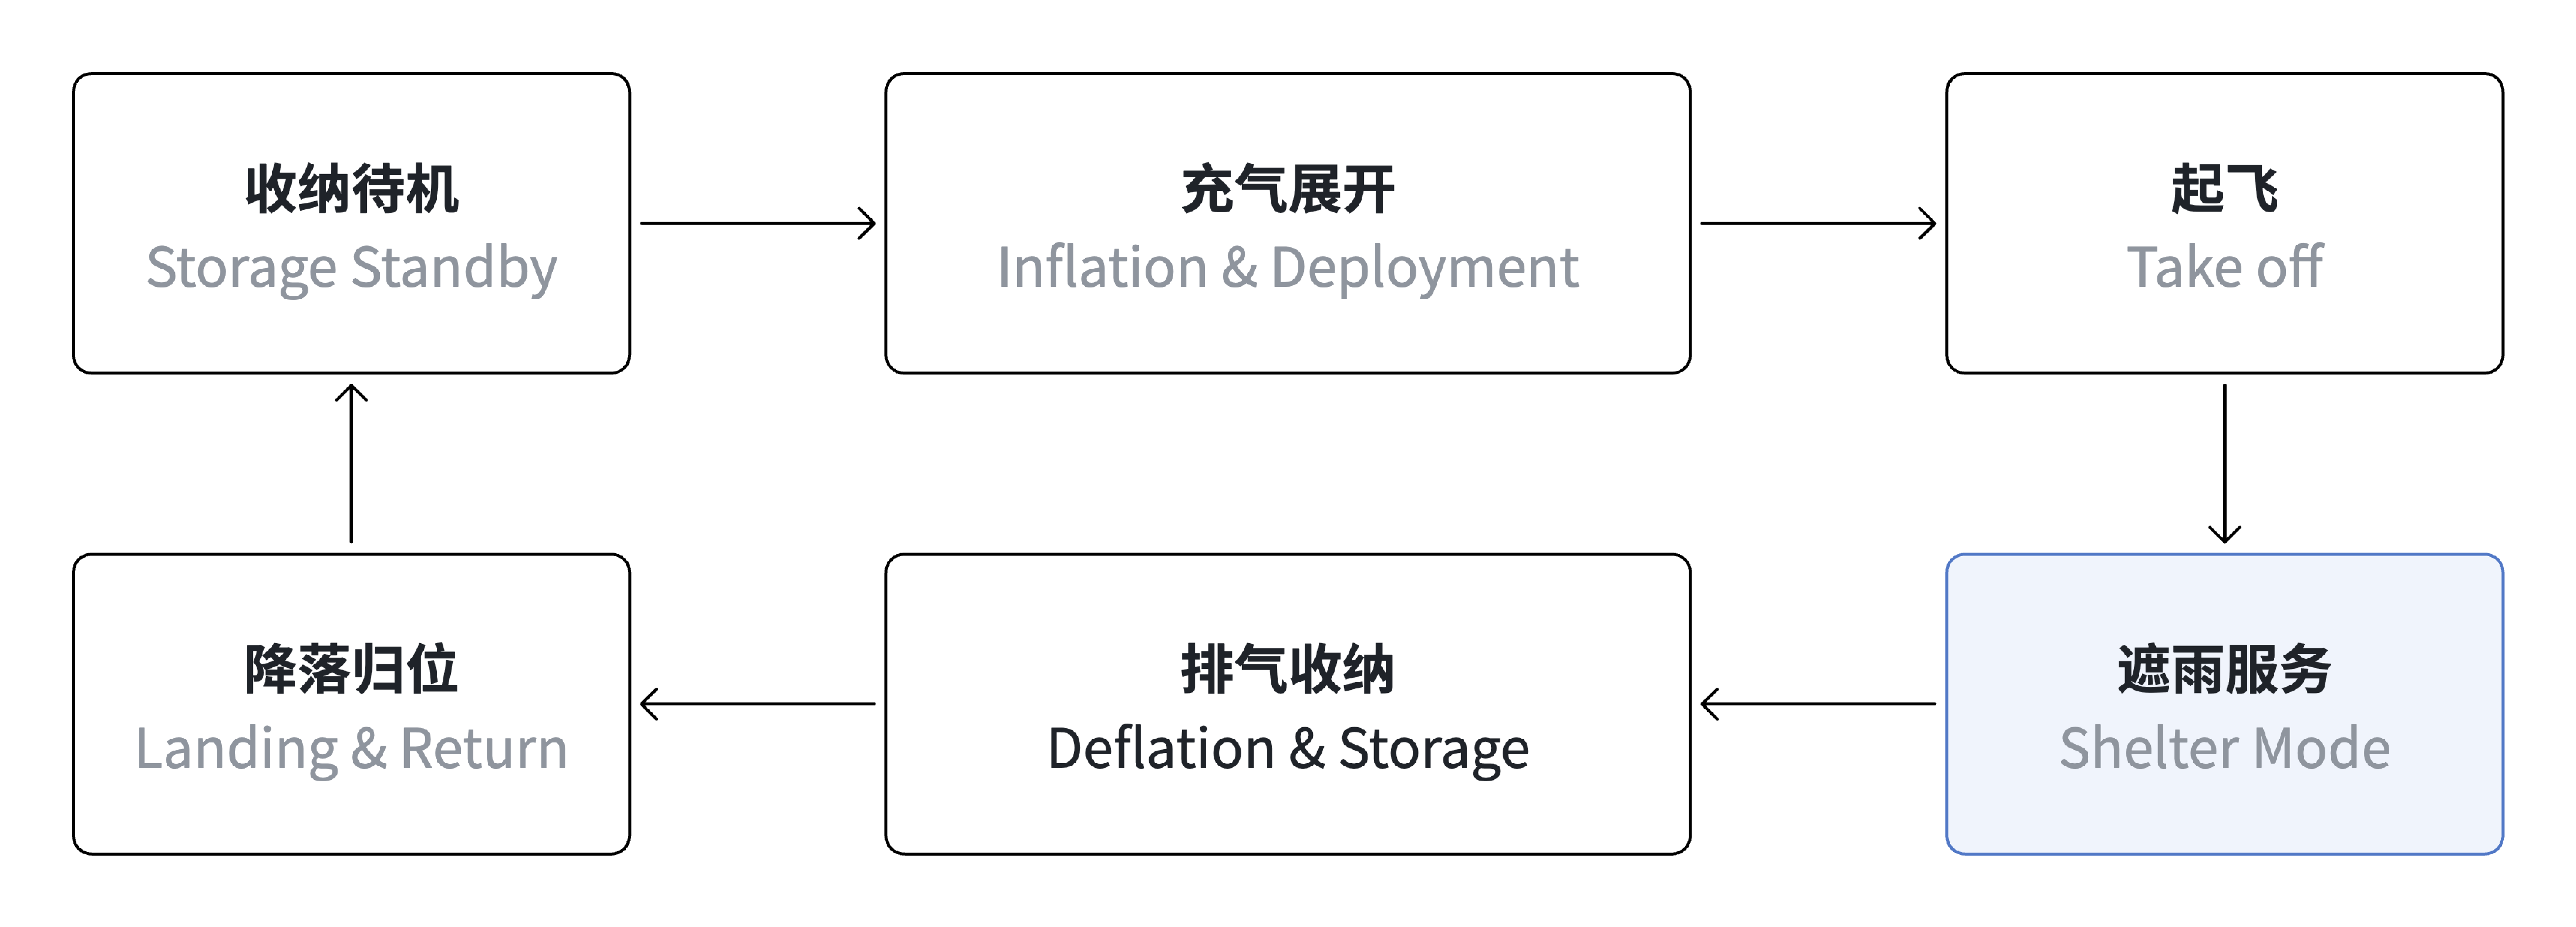
\includegraphics[width=\textwidth]{figures/fig2_2_workflow.png}
%     \caption{飞行雨伞系统六阶段使用流程图}
%     \label{fig:workflow}
% \end{figure}
% ----------------------------------------------------------

\subsection{供电形态设计}

结合实际使用需求，飞行雨伞系统设计了两种互补的供电形态，以适应功能验证与实际出行场景的不同需求，
如表~\ref{tab:power_mode}所示。

\begin{table}[htbp]
    \centering
    \caption{两种供电形态对比}
    \label{tab:power_mode}
    \begin{tabular}{lll}
        \toprule
        对比维度         & 自载电池模式               & 系留供电模式 \\
        \midrule
        供电来源         & 机载6S 1500\,mAh电池       & 地面6S 10000\,mAh电池（有线） \\
        理论续航         & 约3\,min（应急用途）        & $\geq15$\,min \\
        飞行自由度       & 完全无线，机动性强           & 受系留缆线约束（缆长约150\,cm） \\
        用户双手         & 不影响                     & 电源可入包/入口袋，双手完全解放 \\
        主要用途         & 功能验证、自主返航备用电源    & 日常遮雨服务、长时悬停任务 \\
        安全冗余         & 独立供电，无断连风险          & 缆线物理拉力防止失控高飞 \\
        \bottomrule
    \end{tabular}
\end{table}

\textbf{自载电池模式（Onboard Battery Mode）}：
飞行雨伞搭载机载小电池（样机为6S 1500\,mAh），系统完全自主、无线缆束缚。
该模式主要服务于两个场景：一是早期功能验证与短时飞行测试；
二是在系留模式主电源意外断连时，机载电池作为应急备用电源，
为系统提供足够完成一次安全降落或自主返航的动力裕量，有效规避炸机风险。
由于机载电池容量较小，该模式不作为日常服务的主要供电方式。

\textbf{系留供电模式（Tethered Power Mode）}：
飞行器通过轻质供电线缆与地面大容量电池（样机为6S 10000\,mAh）有线连接，
彻底解除了机载电池容量对续航的限制。
地面电源可由用户随身携带（置于背包或裤兜），无需手持，真正实现双手解放。
系留缆线设计长度约150\,cm，满足飞行雨伞在约2\,m悬停高度下的运动自由度，
并在测试阶段通过缆线末端的物理拉力提供额外安全冗余，防止失控高飞。
系留模式是飞行雨伞面向实际出行场景的主要工作形态。

两种供电形态通过插拔电源接口实现快速切换，相互补充，
共同构成飞行雨伞系统完整的能源管理方案。


\section{功能需求与关键性能指标}

\subsection{功能需求分解}

根据使用流程分析，飞行雨伞系统需满足以下核心功能需求：

\begin{itemize}
    \item \textbf{形态重构能力：}系统须能在收纳态与飞行态之间实现可靠的双向切换，
          充气展开过程自动完成，无需人工干预；
    \item \textbf{飞行稳定性：}飞行器需在有效载荷（充气伞体）条件下实现稳定悬停，
          姿态偏差满足服务要求；
    \item \textbf{遮雨有效性：}充气伞面展开后需提供足够的遮蔽面积，
          能够有效覆盖单人的头部及肩部区域；
    \item \textbf{车载适配性：}系统收纳态尺寸需适配车顶或车尾安装空间，
          固定方案安全可靠，不影响车辆正常使用；
    \item \textbf{操作便捷性：}从用户发出指令到飞行器完成起飞悬停的全程时间
          应控制在合理范围内，满足实际出行场景的时间容忍度。
\end{itemize}

\subsection{关键性能指标体系}

基于功能需求，结合工程可行性分析，制定本系统的关键性能指标（KPI）如表~\ref{tab:kpi}所示。

\begin{table}[htbp]
    \centering
    \caption{飞行雨伞系统关键性能指标}
    \label{tab:kpi}
    \begin{tabular}{llll}
        \toprule
        指标类别       & 指标项目         & 设计目标值              & 验证方式 \\
        \midrule
        \multirow{3}{*}{飞行性能}
                      & 悬停稳定性       & 姿态偏差 $\leq \pm5°$   & 飞控日志分析 \\
                      & 推重比           & $\geq 1.5$             & 动力计算+测试 \\
                      & 最大工作高度     & $2.0\sim2.5$\,m        & 实飞验证 \\
        \midrule
        \multirow{2}{*}{续航性能}
                      & 系留模式续航     & $\geq 15$\,min          & 实飞计时 \\
                      & 自载模式续航     & $\geq 3$\,min（应急）   & 实飞计时 \\
        \midrule
        \multirow{2}{*}{遮护性能}
                      & 伞面遮蔽面积     & $\geq 0.40$\,m$^2$      & 几何测量 \\
                      & 防水等级         & 有效阻断垂直降雨         & 功能验证 \\
        \midrule
        \multirow{3}{*}{形态重构}
                      & 充气展开时间     & $\leq 60$\,s            & 计时测试 \\
                      & 排气收纳时间     & $\leq 60$\,s            & 计时测试 \\
                      & 收纳后尺寸       & 厚度 $\leq 5$\,cm       & 实物测量 \\
        \midrule
        \multirow{2}{*}{系统集成}
                      & 起飞准备时间     & $\leq 90$\,s            & 全流程计时 \\
                      & 整机起飞质量     & $\leq 2.0$\,kg（不含地面电源）& 称重 \\
        \bottomrule
    \end{tabular}
\end{table}

上述指标将作为后续各章节设计计算的约束条件与验证基准。
部分指标（如悬停续航时间）将在实验验证章节与理论估算值进行对比分析。


\section{方案论证}

\subsection{充气方案与刚性方案对比分析}

对于实现"可收纳大面积飞行遮护结构"，在工程上有两种基本技术路线：
充气结构方案与刚性折叠结构方案。两种方案的主要特性对比如表~\ref{tab:scheme_compare}所示。

\begin{table}[htbp]
    \centering
    \caption{充气结构方案与刚性折叠方案对比}
    \label{tab:scheme_compare}
    \begin{tabular}{lll}
        \toprule
        对比维度       & 充气结构方案                     & 刚性折叠结构方案 \\
        \midrule
        收纳体积       & 极小（排气后近似零体积）          & 较大（折叠比约1:3$\sim$1:5） \\
        展开方式       & 充气自动展开，操作简单            & 机械铰链折叠，需人工/电动展开 \\
        系统重量       & 轻（气囊薄膜面密度低）           & 重（碳纤维/金属骨架） \\
        结构刚度       & 依赖充气压力，有一定限制          & 高刚度，结构可靠性强 \\
        制作难度       & 低（标准气柱+3D打印节点）        & 高（折叠机构设计加工复杂） \\
        失效模式       & 漏气导致刚度下降                 & 铰链卡死/疲劳断裂 \\
        维修成本       & 低（气柱可替换）                 & 高（金属/碳纤维件加工成本高） \\
        \bottomrule
    \end{tabular}
\end{table}

综合以上对比，充气结构方案在收纳体积、系统重量与制作工艺三个维度上具有明显优势，
与本系统对车载收纳便捷性与轻量化的核心需求高度契合。
刚性折叠方案虽在结构可靠性上略有优势，
但其难以突破的收纳尺寸下限使其无法满足本系统的收纳性能指标。
因此，本文选择充气结构方案作为伞体形态重构的实现路径。

\subsection{旋翼布局方案选型}

多旋翼飞行器的旋翼布局方案直接影响系统的飞行稳定性、控制解耦性与结构集成难度。
针对飞行雨伞系统的伞形载体特征，对以下三种主流布局方案进行分析与比较，
如表~\ref{tab:rotor_compare}所示。

\begin{table}[htbp]
    \centering
    \caption{三种旋翼布局方案对比}
    \label{tab:rotor_compare}
    \begin{tabular}{llll}
        \toprule
        布局方案              & 优势                        & 劣势                     & 适配性评估 \\
        \midrule
        四旋翼X型（标准）     & 控制成熟、开源支持完善       & 抗非对称干扰能力一般      & 中等 \\
        六旋翼（Y6/六轴）     & 冗余度高、抗扰能力强         & 重量增加、结构复杂        & 较低 \\
        四旋翼伞缘分布式      & 伞体即机臂、结构一体化       & 控制与普通四旋翼一致      & \textbf{最优} \\
        \bottomrule
    \end{tabular}
\end{table}

四旋翼伞缘分布式布局将旋翼直接安装于充气伞形结构的周缘，
利用伞体结构本身作为机臂替代，可最大化利用伞形空间并降低系统质心高度。
这是本项目最具针对性的布局方案，也是充气伞形结构的自然几何约束给出的最优解。
同时，四旋翼布局继承了标准四旋翼完善的PX4飞控支持，
降低了控制系统的开发门槛。
综合考虑控制成熟度、结构重量与对本系统伞形载体的适配性，
本文选择\textbf{四旋翼伞缘分布式布局}作为动力系统布局方案。
旋翼具体安装位置与重心匹配分析将在第四章详细展开。


\section{系统总体架构}

飞行雨伞系统由四个子系统组成，各子系统相互协同，共同支撑完整工作流程的实现。

% ----------------------------------------------------------
% [图片占位 Fig.2.3] ★需要制作★
% 内容：系统总体架构图（四个子系统的关系框图）
%   四个方框：充气伞体系统、多旋翼动力系统、嵌入式飞控系统、车载平台系统
%   用双向箭头或单向箭头表示子系统间的能量/信号/结构依赖关系
%   建议用draw.io或PowerPoint绘制
% \begin{figure}[htbp]
%     \centering
%     \includegraphics[width=0.80\textwidth]{figures/fig2_3_architecture.png}
%     \caption{飞行雨伞系统总体架构图}
%     \label{fig:architecture}
% \end{figure}
% ----------------------------------------------------------

\subsection{充气伞体系统}

充气伞体系统是本项目的核心创新载体，承担形态重构与遮雨防护两项核心功能。
该子系统包括：气囊本体（薄壁气柱，构成伞形骨架与遮护面）、
PLA节点连接件（维持伞形几何形态）、
充气接口（与充气子系统对接）、
以及TPU伞面（提供遮雨遮阳功能）。
充气伞体系统的详细设计见第三章。

\subsection{多旋翼动力系统}

多旋翼动力系统为飞行器提供垂直升力与姿态控制所需的力矩输出，
由四组无刷电机（SIRIUS 2306.5-1850KV）、
电子调速器（ESC）、桨叶（51366 MCK v3）
与供电系统（机载电池或地面系留电源）组成。
动力系统的选型基于整机质量预算与悬停升力需求的理论计算结果，
具体计算过程见第四章。

\subsection{嵌入式飞行控制系统}

嵌入式飞行控制系统以Pixhawk 6C开源飞控为核心计算平台，
搭载NuttX实时操作系统，集成IMU（惯性测量单元）、气压计、磁力计等传感器，
负责完成传感器数据融合、姿态估计、飞行控制律解算与电机PWM指令输出。
PX4固件提供了成熟的多旋翼姿态控制回路与位置控制回路，
是系统实现稳定悬停的核心保障。飞控系统架构与参数整定过程见第五章。

\subsection{车载平台系统}

车载平台系统承担系统的部署基础功能，包括：
承载结构（固定于车顶行李架或车尾的安装基板）、
起降区域（为飞行器提供标定的起飞与降落落点）、
充气设备（车载12\,V微型气泵，通过快接接口与气囊连接）、
以及电源接口（通过车载12\,V电源为充气设备供电）。
车载平台的详细设计见第六章。


\section{本章小结}

本章从应用场景出发，完成了飞行雨伞系统的需求分析与总体方案设计。
通过对目标场景的系统梳理，提出了涵盖六个阶段的完整使用流程，
并在此基础上设计了自载电池与系留供电两种互补的供电形态，
以适应功能验证与实际使用场景的不同需求。
本章建立了系统关键性能指标体系，并通过充气方案与刚性方案的对比论证、
旋翼布局的选型分析，确定了本系统的核心技术路线。
在此基础上，提出了由充气伞体系统、多旋翼动力系统、
嵌入式飞行控制系统与车载平台系统四个子系统构成的总体架构，
为后续各章节的详细设计提供了清晰的工程框架。    % 第二章 系统需求分析与总体方案
% ============================================================
% 第三章 充气伞形结构设计
% ============================================================

\chapter{充气伞形结构设计}

\section{充气结构力学基础}

\subsection{薄壁充气结构受力原理}
充气结构（Pneumatic Inflatable Structure）是一类依靠内部气体压力维持形态与结构刚度的柔性结构体系。
其基本工作原理可通过薄壁压力容器理论加以描述：当气囊内部气体压力 $p$ 大于外部大气压时，
气囊壁面承受周向（环向）拉应力与轴向拉应力，在两者的共同作用下气囊维持充气形态并具备抵抗外力变形的能力。
对于简化为圆柱形薄壁气囊的情形，气囊壁面所受环向应力 $\sigma_\theta$ 与轴向应力 $\sigma_z$ 分别为：
\begin{equation}
    \sigma_\theta = \frac{p \cdot r}{t}
    \label{eq:hoop_stress}
\end{equation}
\begin{equation}
    \sigma_z = \frac{p \cdot r}{2t}
    \label{eq:axial_stress}
\end{equation}
其中 $p$ 为充气表压（Pa），$r$ 为气囊内半径（m），$t$ 为气囊壁厚（m）。
由此可见，环向应力是轴向应力的两倍，气囊最容易沿轴向方向开裂，
这也是气囊材料选型中需要重点考量环向强度的原因。

\subsection{充气压力与结构刚度的关系}
充气结构的等效抗弯刚度随充气压力的增大而提高。
在小变形假设下，充气圆柱梁在承受外部横向载荷（如飞行器的结构重力与旋翼推力）时，其内部受力状态与弯曲变形特征如图~\ref{fig:inflatable_bending}所示\cite{Sun2024}。

\begin{figure}[htbp]
    \centering
    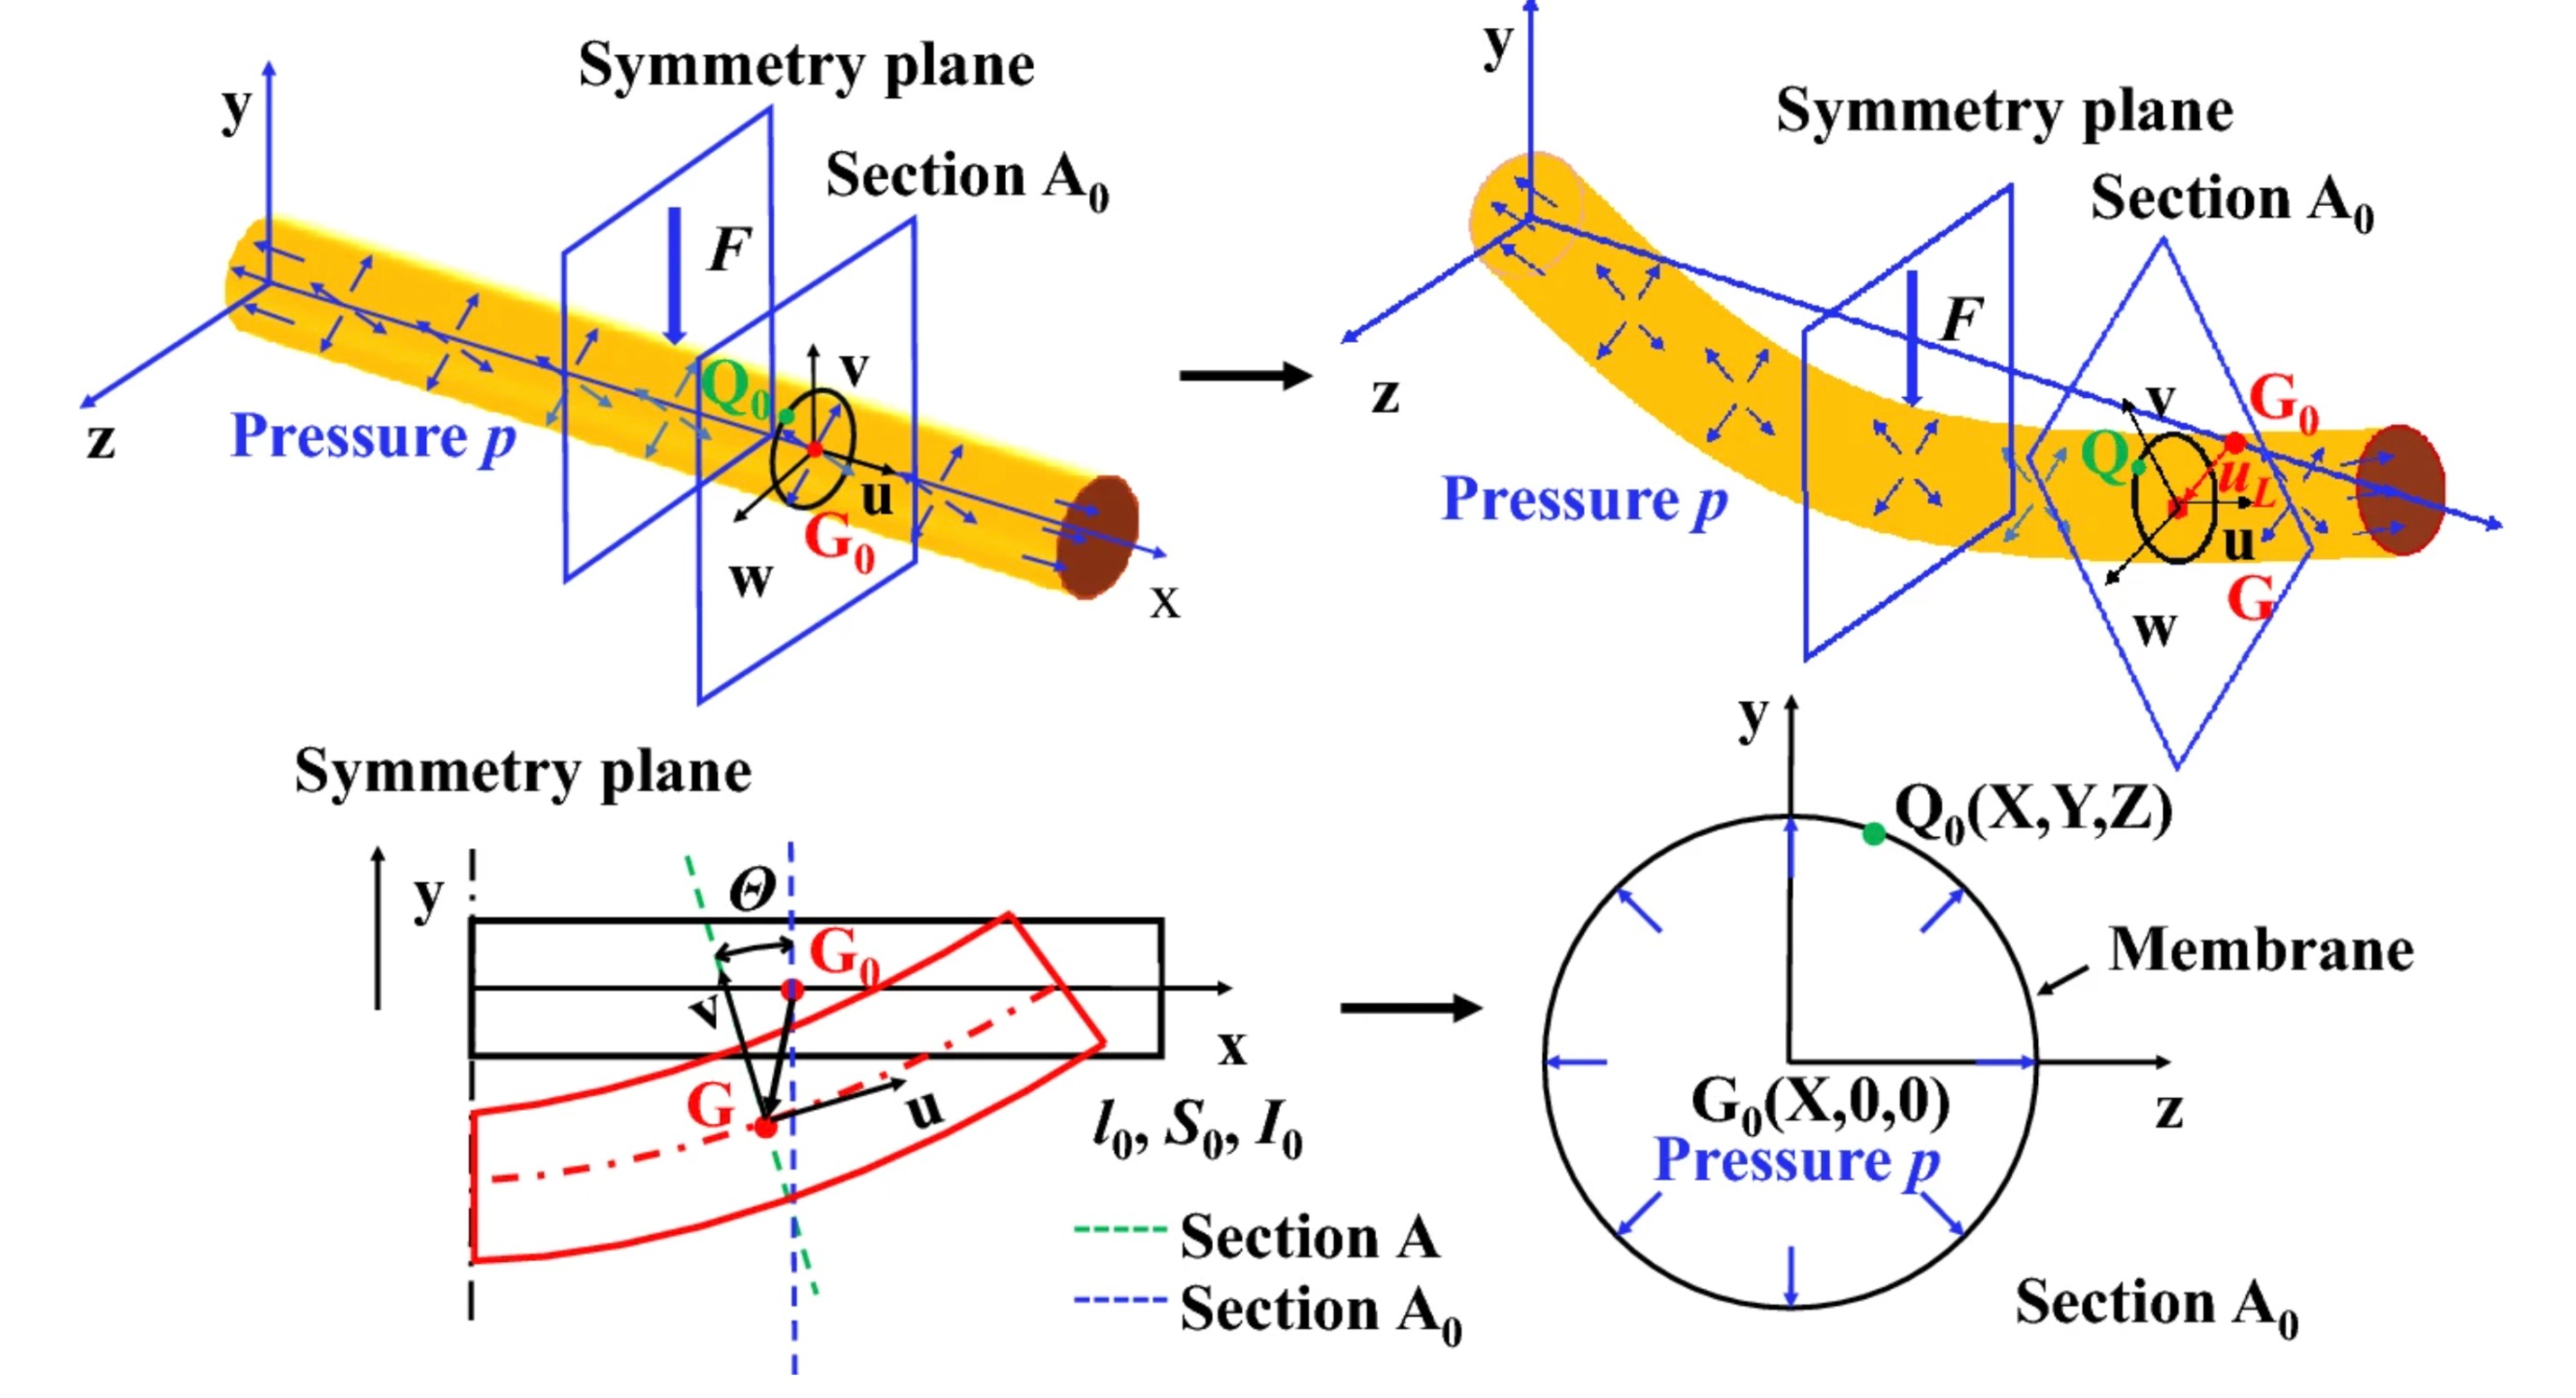
\includegraphics[width=0.85\textwidth]{figures/fig3_1_inflatable_bending.pdf}
    \caption{圆柱形充气梁弯曲受力模型与截面变形示意图（图片来源：Sun 等, 2024~\cite{Sun2024}）}
    \label{fig:inflatable_bending}
\end{figure}

如图~\ref{fig:inflatable_bending}右下角的截面图所示，内部气体压力 $p$ 均匀作用于气囊内壁，使膜材处于预张紧状态。
充气压力越高，气囊壁面初始张力越大，结构对横向弯曲载荷的抵抗能力越强；
当充气压力不足时，气囊将在弯曲载荷下出现局部塌陷，失去承载能力。
近年来，Sun 等人的研究进一步表明，充气梁在弯曲过程中的剪切效应高度依赖于截面特征，且内压的变化会显著改变充气梁的几何参数与动态刚度\cite{Sun2024}。
这一特性决定了充气结构在使用过程中需要维持一定的最低工作气压，以保证结构刚度满足飞行载荷要求。

本文所采用的充气气柱为市售标准快递气柱，如图~\ref{fig:aircolumn_compare}所示，其充气后圆柱直径约为 $1.7\sim2.0$\,cm，
充气工作气压约为 $0.05\sim0.1$\,MPa（表压）。
气柱材料为PA（尼龙）复合薄膜，具有良好的气密性、一定的柔韧性以及对水汽的阻隔能力，
能够应对户外雨天使用场景。

% ----------------------------------------------------------
% [图片占位 Fig.3.2] ★需要拍摄★
% 内容：气柱实物对比照片
%   左：排气折叠状态（扁平薄膜状）
%   右：充气后圆柱状态，旁边放尺子标注直径约1.9cm
%   用手机拍摄即可，光线均匀，白色背景最佳
\begin{figure}[htbp]
    \centering
    \includegraphics[width=0.65\textwidth]{figures/fig3_2_aircolumn_compare.pdf}
    \caption{快递气柱排气状态（左）与充气状态（右）对比}
    \label{fig:aircolumn_compare}
\end{figure}

% ----------------------------------------------------------



\section{充气伞形骨架结构设计}

\subsection{结构概念与设计思路}

飞行雨伞的充气骨架系统承担两项核心功能：其一，作为多旋翼飞行器的机体骨架，
为四组旋翼动力单元提供安装位置和结构支撑；其二，作为伞面的支撑框架，
维持TPU伞面的展开形态，实现有效的遮雨遮阳防护。
骨架系统的整体三维结构如图~\ref{fig:cad_overview}所示。

\begin{figure}[htbp]
    \centering
    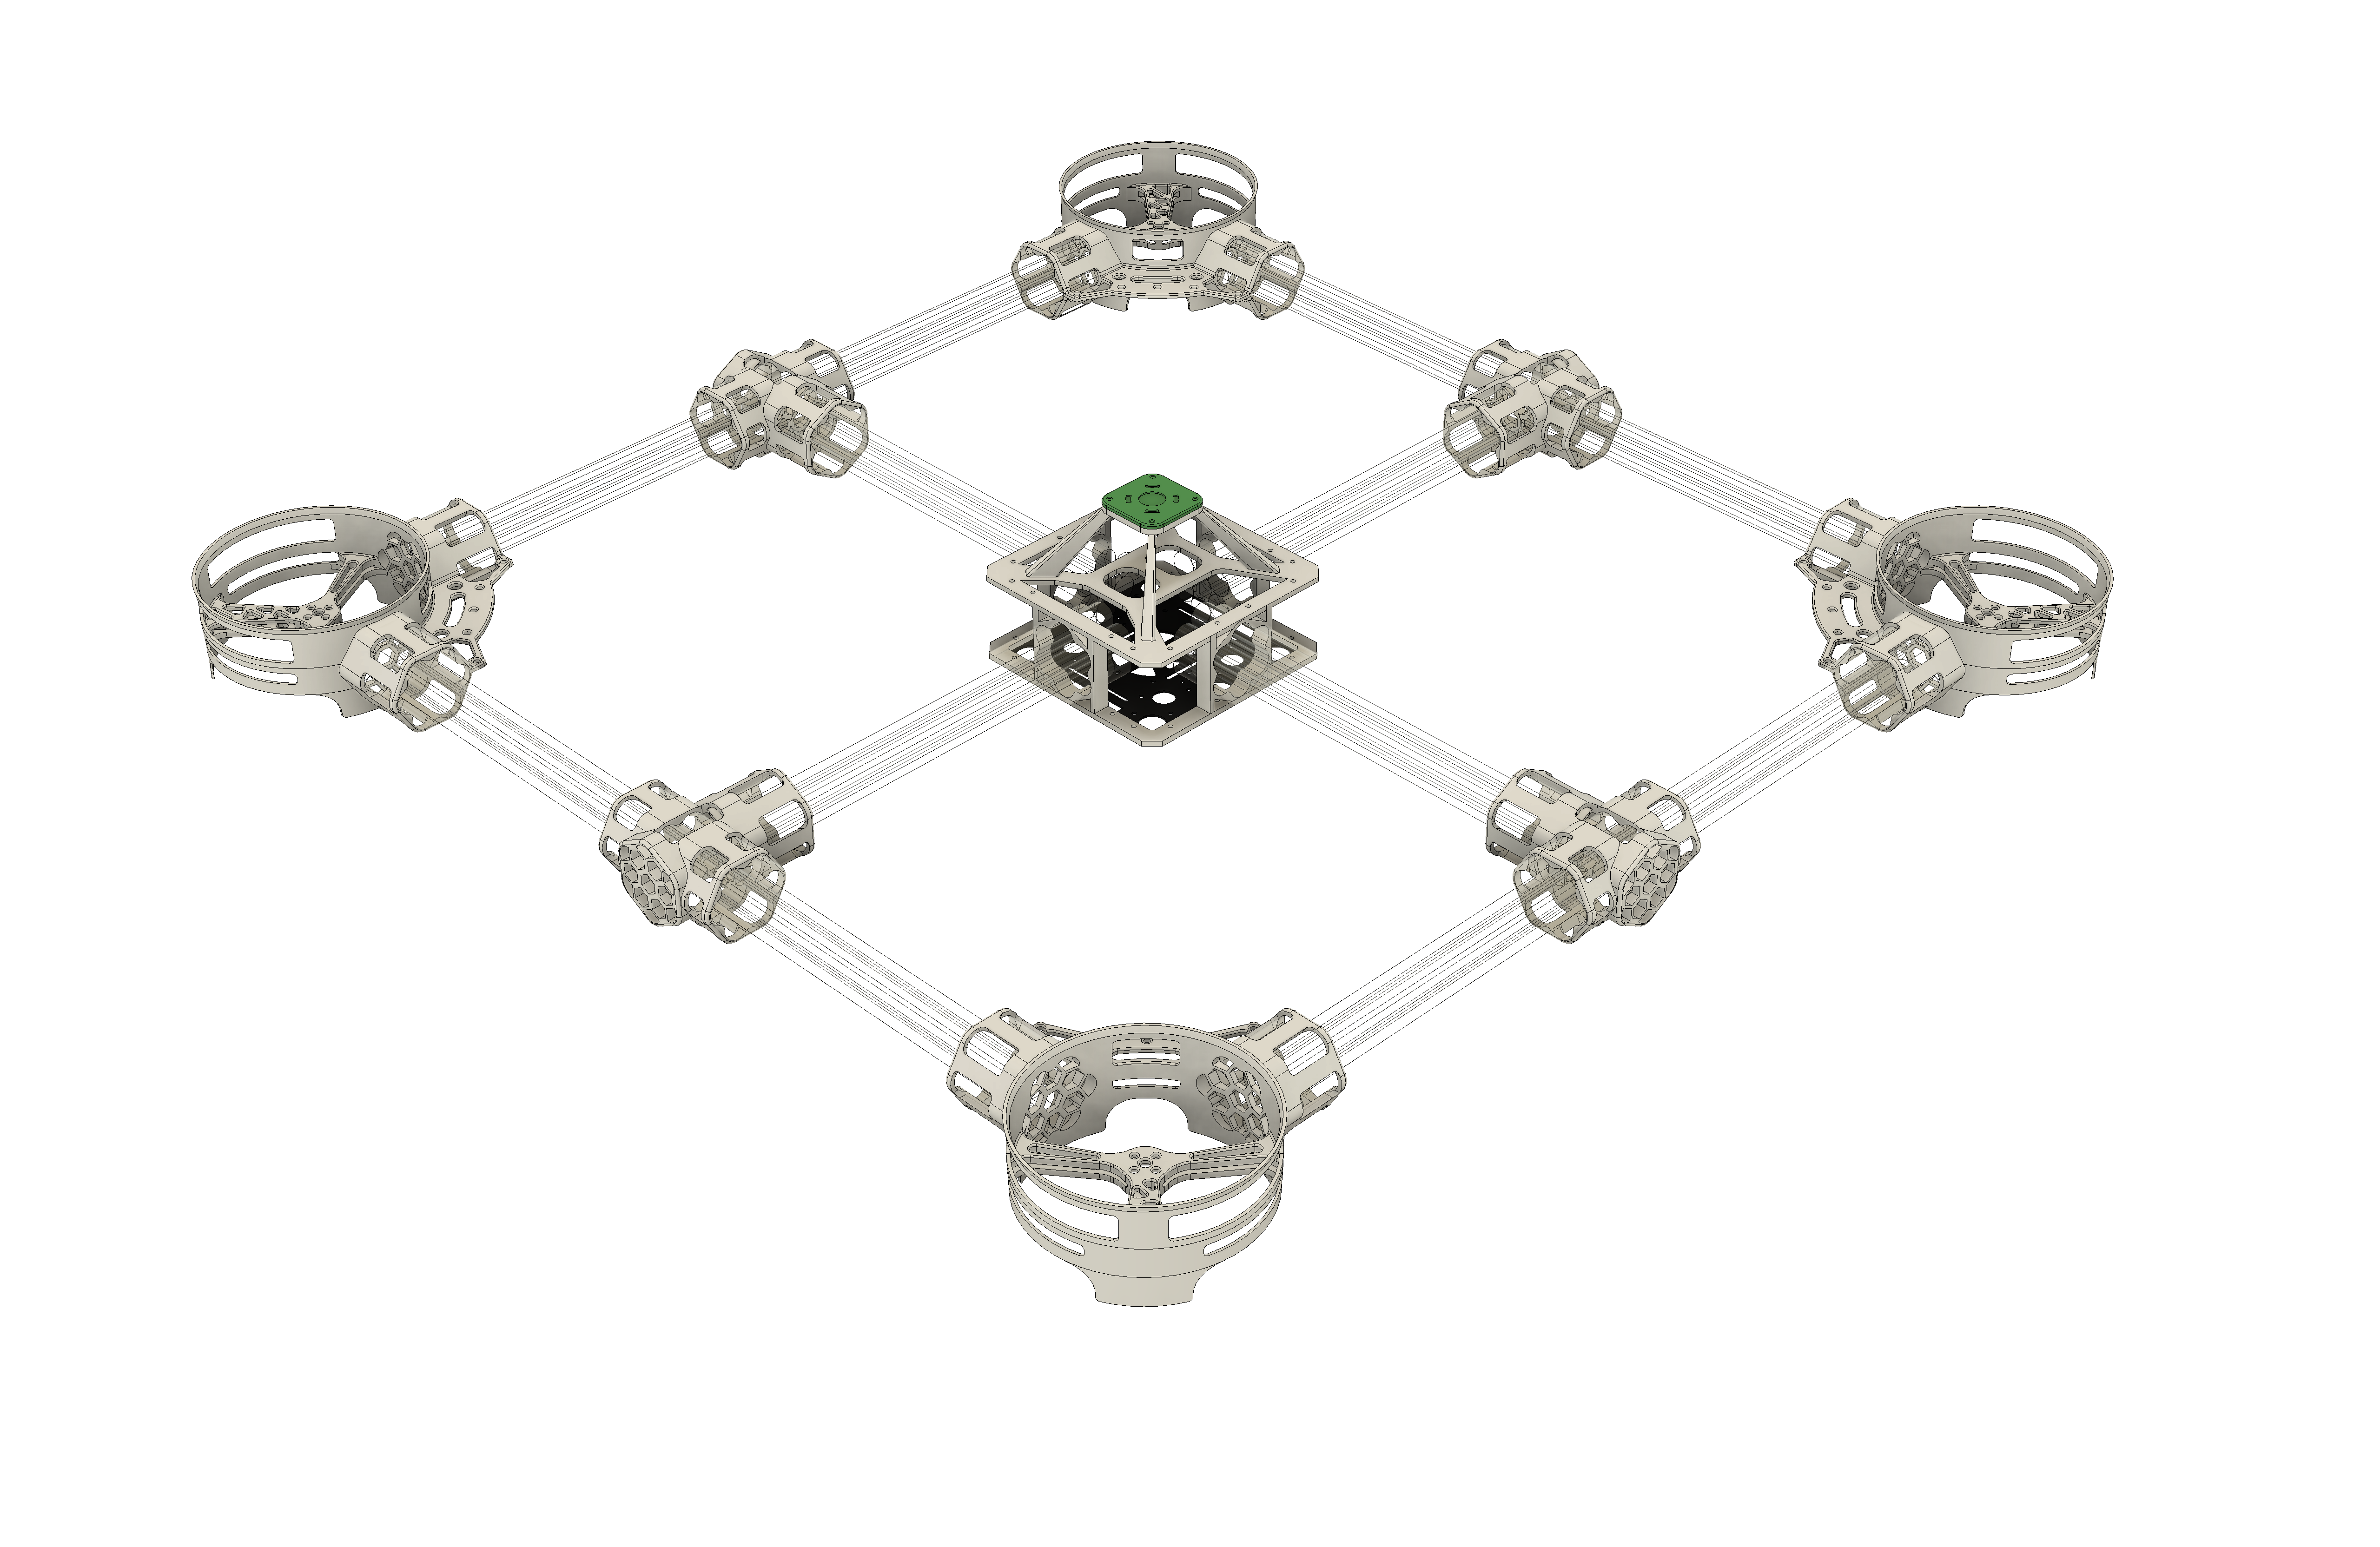
\includegraphics[width=0.80\textwidth]{figures/fig3_1_cad_overview.png}
    \caption{充气伞形骨架系统整体三维结构（Fusion 360）}
    \label{fig:cad_overview}
\end{figure}

本系统采用\textbf{气柱-节点模块化骨架}设计思路：以标准快递气柱作为承力杆件，
以 PLA（聚乳酸）3D 打印节点作为连接与固定元件，构成正方形平面桁架式骨架结构。
气柱在排气状态下可完全压缩折叠，体积接近零；充气后具备一定的结构刚度，
能够承受旋翼推力产生的局部集中载荷。
系统中\textbf{不使用任何刚性碳纤维或金属结构件}，气柱本身即是机臂上的唯一承力构件，
"充气即成形、排气即收纳"的形态切换由此得以实现。

\subsection{骨架几何构型}

骨架采用正方形平面布局，四角各安装一套旋翼动力单元（含电机、电调与3D打印旋翼保护架）。
各旋翼单元通过气柱与相邻节点连接件对接，形成闭合的正方形框架，
如图~\ref{fig:frame_cad}所示。骨架的主要几何参数如表~\ref{tab:frame_dimensions}所示。

\begin{table}[htbp]
    \centering
    \caption{骨架主要几何参数}
    \label{tab:frame_dimensions}
    \begin{tabular}{llll}
        \toprule
        参数             & 设计值    & 实测值       & 说明 \\
        \midrule
        骨架外框边长      & 888\,mm  & 870\,mm     & 气柱充气后自然收缩 \\
        对角旋翼轴距      & 1256\,mm & 1230\,mm    & 对角线尺寸 \\
        单边气柱标称长度   & 600\,mm  & 560\,mm     & 充气后收缩约7\% \\
        单气柱充气直径    & 约20\,mm & 17$\sim$20\,mm & 标准快递气柱 \\
        旋翼保护架外径    & 146\,mm  & 146\,mm     & 3D打印PLA \\
        \bottomrule
    \end{tabular}
\end{table}

设计值与实测值存在约2\%的尺寸偏差，主要来源于气柱充气后的轴向收缩效应
以及节点接口处气柱端部薄膜堆积。在工程应用中，以实测值作为结构性能分析的基准参数。

% ----------------------------------------------------------
% [图片占位 Fig.3.3] ★可直接使用已有截图★
% 内容：骨架CAD设计俯视图（带尺寸标注）
%   即之前发给我的"888.866mm"测量截图
%   建议：在CAD中再额外标注对角线1256mm和保护圈直径146mm后截图
%   裁去右侧属性面板，只保留模型区域
\begin{figure}[htbp]
    \centering
    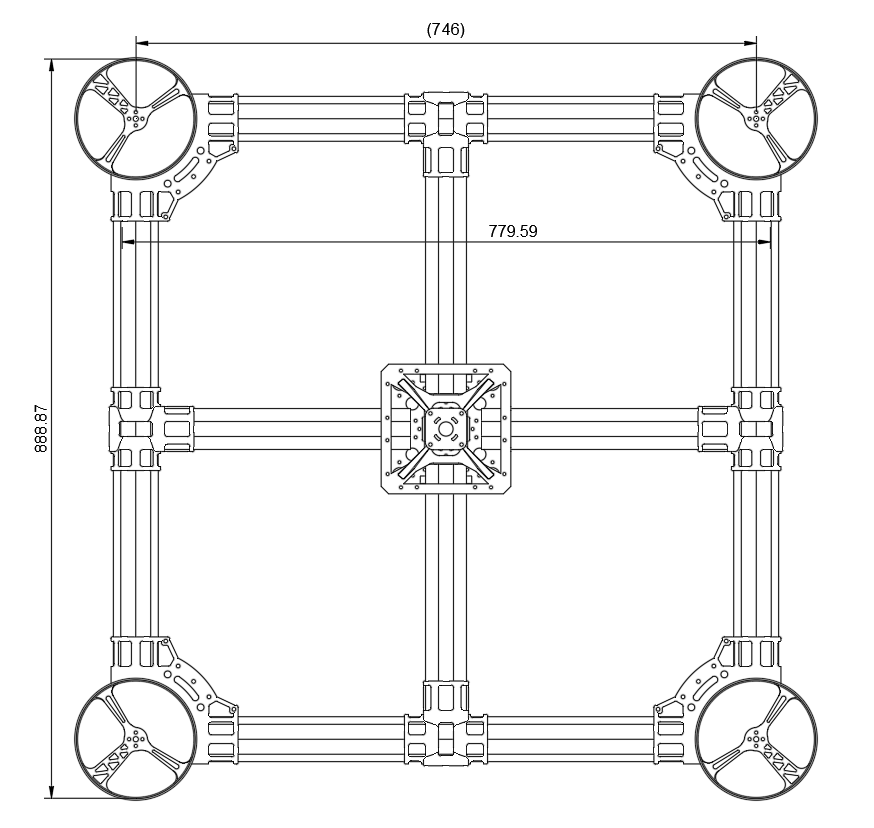
\includegraphics[width=0.75\textwidth]{figures/fig3_3_frame_cad.png}
    \caption{飞行雨伞骨架CAD设计俯视图}
    \label{fig:frame_cad}
\end{figure}
% ----------------------------------------------------------

\subsection{气柱布置方案与连接设计}
每条骨架边由七根标准快递气柱单元卷绕组合而成，气柱两端通过PLA节点连接件固定。
七根气柱按蜂窝式排列——中心1根、外围6根紧密围绕——充气后各气柱单元相互挤压，
自然形成近似正六边形的组合截面，等效外径约为 54.2\,mm。
这种多气柱并联组合方案在单个气柱单元发生漏气时，
其余气柱仍可维持骨架基本形态，具备一定的冗余容错能力。

节点连接件同时承担以下功能：气柱端口密封固定、相邻两边骨架的正交对接、
旋翼安装座集成（四角节点），以及中心飞控安装平台的连接接口。

为确保柔性气柱束与刚性PLA节点之间的连接强度，本系统设计了与七根气柱卷绕截面相匹配的
专用孔道结构。如图~\ref{fig:node_section}所示，节点连接件的内孔截面设计为
由三个半径 $R=10$\,mm 的外凸圆弧与半径 $R=5$\,mm 的内凹圆弧交替构成的三叶形轮廓，
相邻凸起间夹角为 120°。
三叶形的三个凸起分别对应七根气柱蜂窝截面外围的三对气柱，
孔道轮廓与气柱束充气后的自然膨胀形态高度吻合，形成有效的几何限位。
在实际装配中（如图~\ref{fig:node_assembly_real}所示），
气柱束穿过三叶形孔道后，在孔壁接触面处注入热熔胶进行二次固定，
冷却固化后同时起到增强轴向抗拉强度与辅助密封的作用。

\begin{figure}[htbp]
    \centering
    \begin{minipage}[b]{0.48\textwidth}
        \centering
        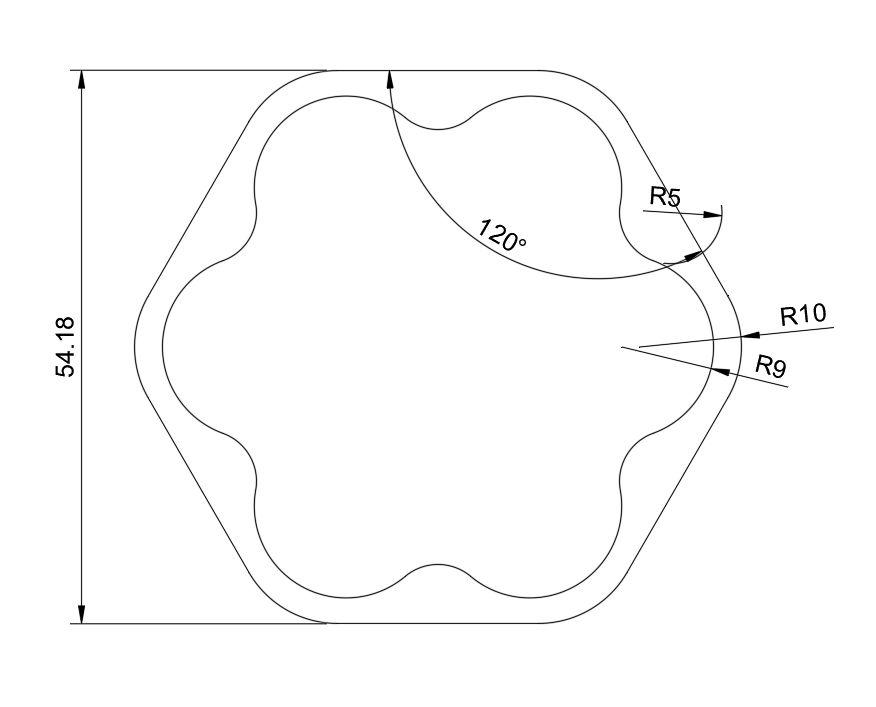
\includegraphics[width=\textwidth]{figures/fig3_node_section_cad.png}
        \caption{节点连接件截面CAD设计图}
        \label{fig:node_section}
    \end{minipage}
    \hfill
    \begin{minipage}[b]{0.48\textwidth}
        \centering
        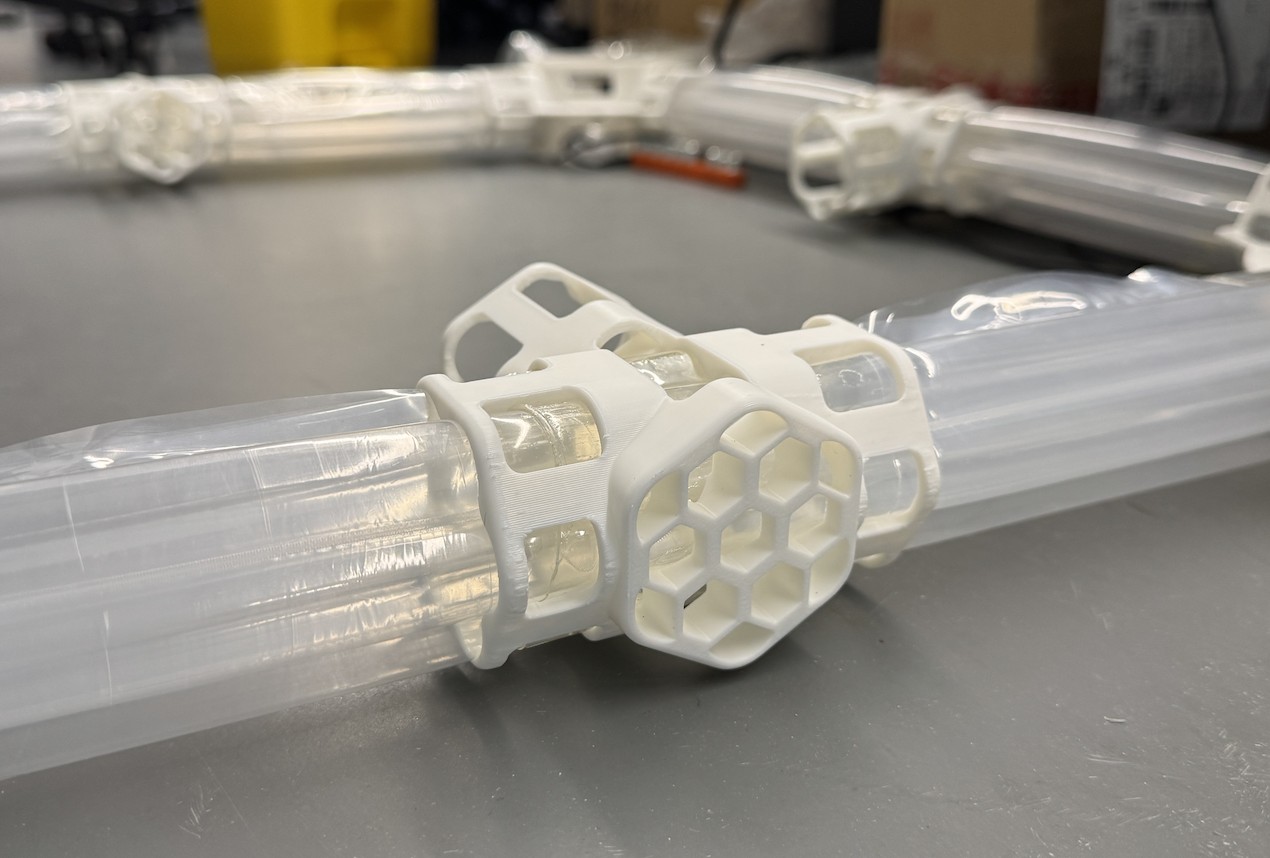
\includegraphics[width=\textwidth]{figures/fig3_node_assembly_real.png}
        \caption{气柱与PLA节点连接件实物装配图}
        \label{fig:node_assembly_real}
    \end{minipage}
\end{figure}

在实际装配中（如图~\ref{fig:node_assembly_real}所示），
气柱穿过PLA连接件的孔道，孔道的几何形状对气柱形成了有效的物理限位，
防止气柱在受力时发生径向滑脱或扭转。
同时，在气柱与PLA孔壁的接触面之间注入热熔胶进行二次固定。
热熔胶冷却固化后，不仅增强了连接的轴向抗拉强度，还起到了进一步的密封作用。
全部PLA节点结构件由FDM工艺3D打印制作，材料为PLA。
这种多气柱并联设计在单个气囊发生漏气时，其余气柱仍可维持骨架基本形态，具备一定的冗余容错能力。

\subsection{骨架尺寸参数验证}
骨架的详细尺寸参数通过CAD装配模型进行了精确验证。
图~\ref{fig:node_dimensions}展示了T型节点连接件的详细尺寸，
其整体高度为 600\,mm，中心套筒宽度为 100\,mm。

\begin{figure}[htbp]
    \centering
    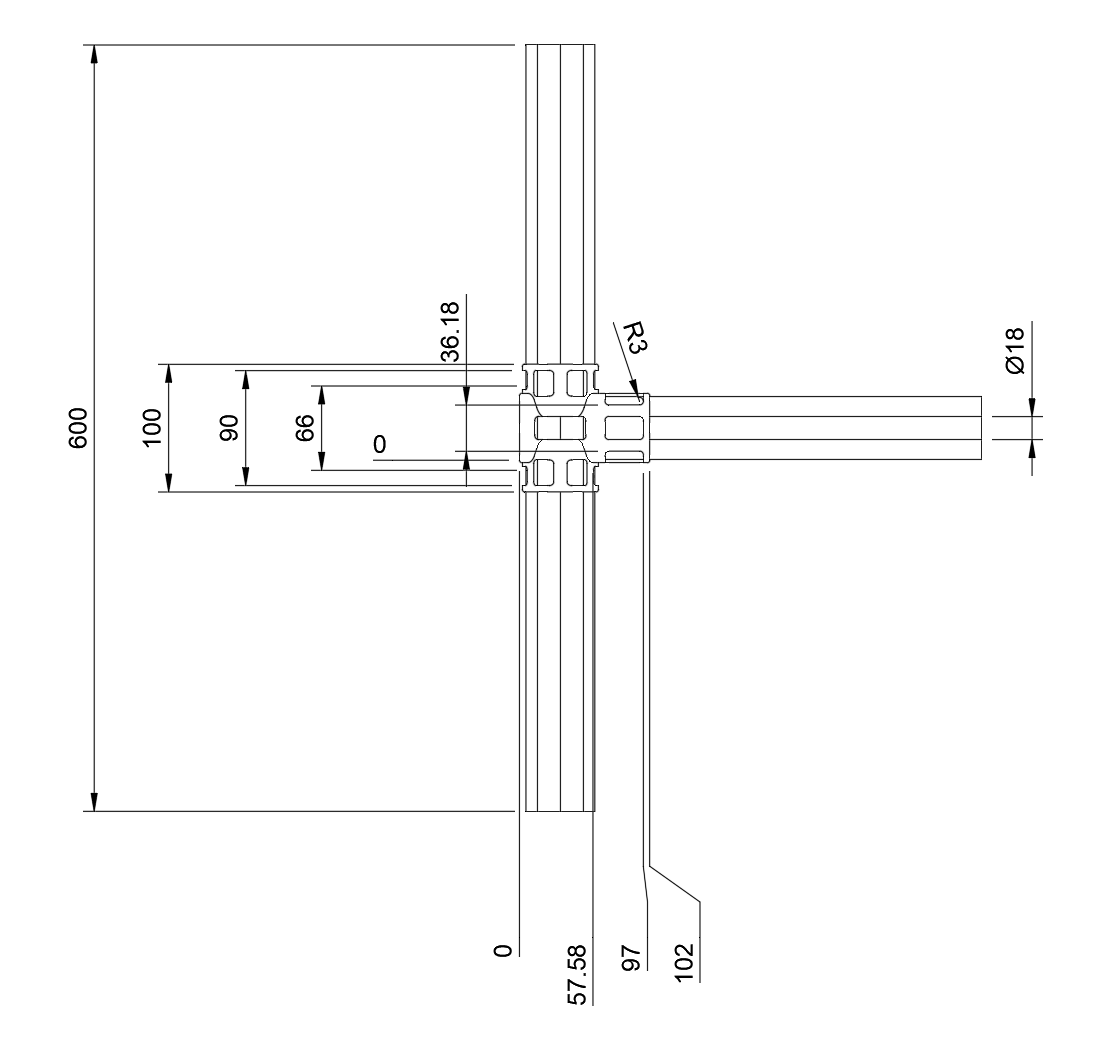
\includegraphics[width=0.75\textwidth]{figures/fig3_node_dimensions.png}
    \caption{T型节点连接件尺寸标注图}
    \label{fig:node_dimensions}
\end{figure}

图~\ref{fig:frame_assembly_dim}展示了骨架装配的整体尺寸标注，
骨架中心到旋翼保护圈中心的X方向距离为 338\,mm，Y方向距离为 333.45\,mm，
即旋翼的X方向轴距为 676\,mm，Y方向轴距为 666.9\,mm；
中心固定架相对骨架平面的抬高量为 76.53\,mm。

\begin{figure}[htbp]
    \centering
    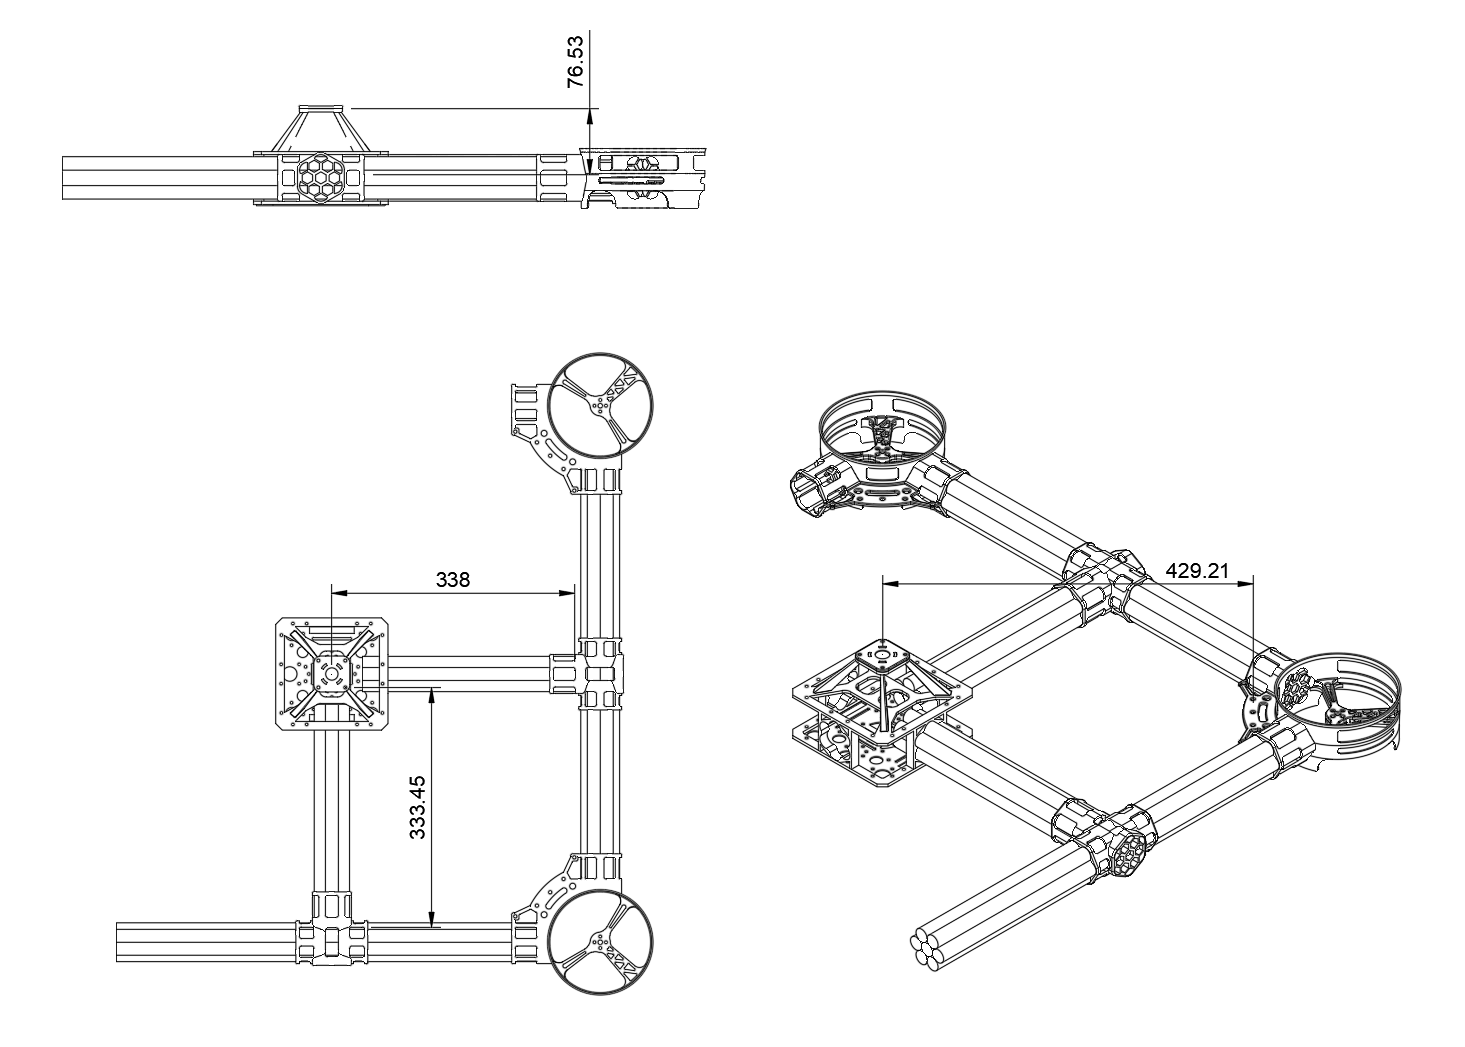
\includegraphics[width=0.85\textwidth]{figures/fig3_frame_assembly_dim.png}
    \caption{骨架装配尺寸标注图}
    \label{fig:frame_assembly_dim}
\end{figure}


% ----------------------------------------------------------
\section{TPU伞面设计}
\subsection{伞面材料选型}
伞面采用热塑性聚氨酯弹性体（TPU，Thermoplastic Polyurethane）薄膜材料。
选用TPU的主要依据如下：
\begin{itemize}
    \item \textbf{防水性能：}TPU薄膜具有优异的防水性能，在遮雨功能场景下表现可靠；
    \item \textbf{轻量化：}TPU薄膜面密度低，同等覆盖面积下重量远小于传统伞布；
    \item \textbf{柔性收纳：}TPU薄膜柔软可折叠，排气后可随气柱骨架一同压缩收纳；
    \item \textbf{耐候性：}TPU对紫外线、温度变化具有良好的适应性，适合户外长期使用。
\end{itemize}

\subsection{伞面几何设计与遮蔽面积}
TPU伞面铺设于骨架气柱的外侧并粘合固定，其水平投影形状为正方形。
伞面有效遮蔽边长取骨架外侧气柱外边缘到对边气柱外边缘的距离，
由CAD模型实测得该边长为 $L_{\text{shelter}} = 779.59$\,mm（约 77.96\,cm）。
伞面水平投影面积（正投影遮蔽面积）为：
\begin{equation}
    S = L_{\text{shelter}}^2 = (0.77959)^2 \approx 0.608\,\text{m}^2
    \label{eq:umbrella_area}
\end{equation}
相比之下，成人头肩部的遮蔽需求约为 $0.25\sim0.30$\,m$^2$。
本系统 0.608\,m$^2$ 的有效遮蔽面积在悬停精度良好的前提下可提供充裕的遮护裕量，
遮护面积冗余约 103\%\,$\sim$\,143\%。

\subsection{伞面倾角设计}
考虑到飞行雨伞在实际使用中需覆盖用户的头部及肩部区域，
伞面设计为具有一定向下倾斜角度的非水平结构，使伞面形成类似传统雨伞的拱形遮蔽形态，
同时有利于积水沿伞面边缘自然流下，避免积水在伞面中心造成附加质量。
伞面倾角由中心固定架的抬高量 $h$ 与水平投影距离 $d$ 共同决定。

根据图~\ref{fig:frame_assembly_dim}的侧视图尺寸标注，
中心固定架将伞面中心相对骨架平面抬高 $h = 76.53$\,mm。
水平投影距离取中心点到骨架边框中点的投影距离（即半轴距），
取X、Y方向的平均值 $d_{\text{avg}} = (338 + 333.45)/2 = 335.725$\,mm。
平均伞面倾角 $\alpha$ 计算如下：
\begin{equation}
    \alpha = \arctan\!\left(\frac{h}{d_{\text{avg}}}\right)
           = \arctan\!\left(\frac{76.53}{335.725}\right)
           \approx 12.8°
    \label{eq:tilt_angle}
\end{equation}
本系统伞面倾角约为 12.8°，
与传统雨伞伞面倾角（通常为 $10°\sim15°$）高度吻合，
能够完美满足积水引导与遮蔽形态的功能要求。


% ----------------------------------------------------------
% [图片占位 Fig.3.5] ★需要制作★
% 内容：伞面倾角设计侧视示意图
%   元素：水平骨架线、中心固定架（竖线）、伞面（从固定架顶端向四周倾斜的弧线）
%   标注：倾角15°、伞面覆盖直径72cm
%   用PowerPoint绘制即可，简洁清晰为主
% \begin{figure}[htbp]
%     \centering
%     \includegraphics[width=0.60\textwidth]{figures/fig3_5_umbrella_tilt.png}
%     \caption{伞面倾角设计示意图（侧视），倾角约15°}
%     \label{fig:umbrella_tilt}
% \end{figure}
% ----------------------------------------------------------


\section{充气展开系统}

\subsection{充气方式与设备选型}
本系统的充气骨架采用分腔充气设计：骨架气柱与伞面气柱分别独立充气，互不干扰。
充气操作通过骨架上预留的充气阀接口完成，使用标准气嘴与充气泵对接。

快递气柱的充气原理如图~\ref{fig:aircolumn_inflate} 所示。
气柱内部设有一条贯通全长的公共主气道，充气时气体由充气嘴进入主气道
并沿其横向流动；主气道沿途通过若干单向止回阀与各独立气室相连，
气体依次经由单向阀充入各气室，使气室膨胀成型。
气室内压达到平衡后，单向阀在内外压差作用下自动关闭，
各气室独立密封；多余气体经主气道末端排出。
这种结构还带来一个附带优点：即便个别气室破损，
其余气室仍可维持充气状态，不会导致整体骨架失效。

\begin{figure}[htbp]
    \centering
    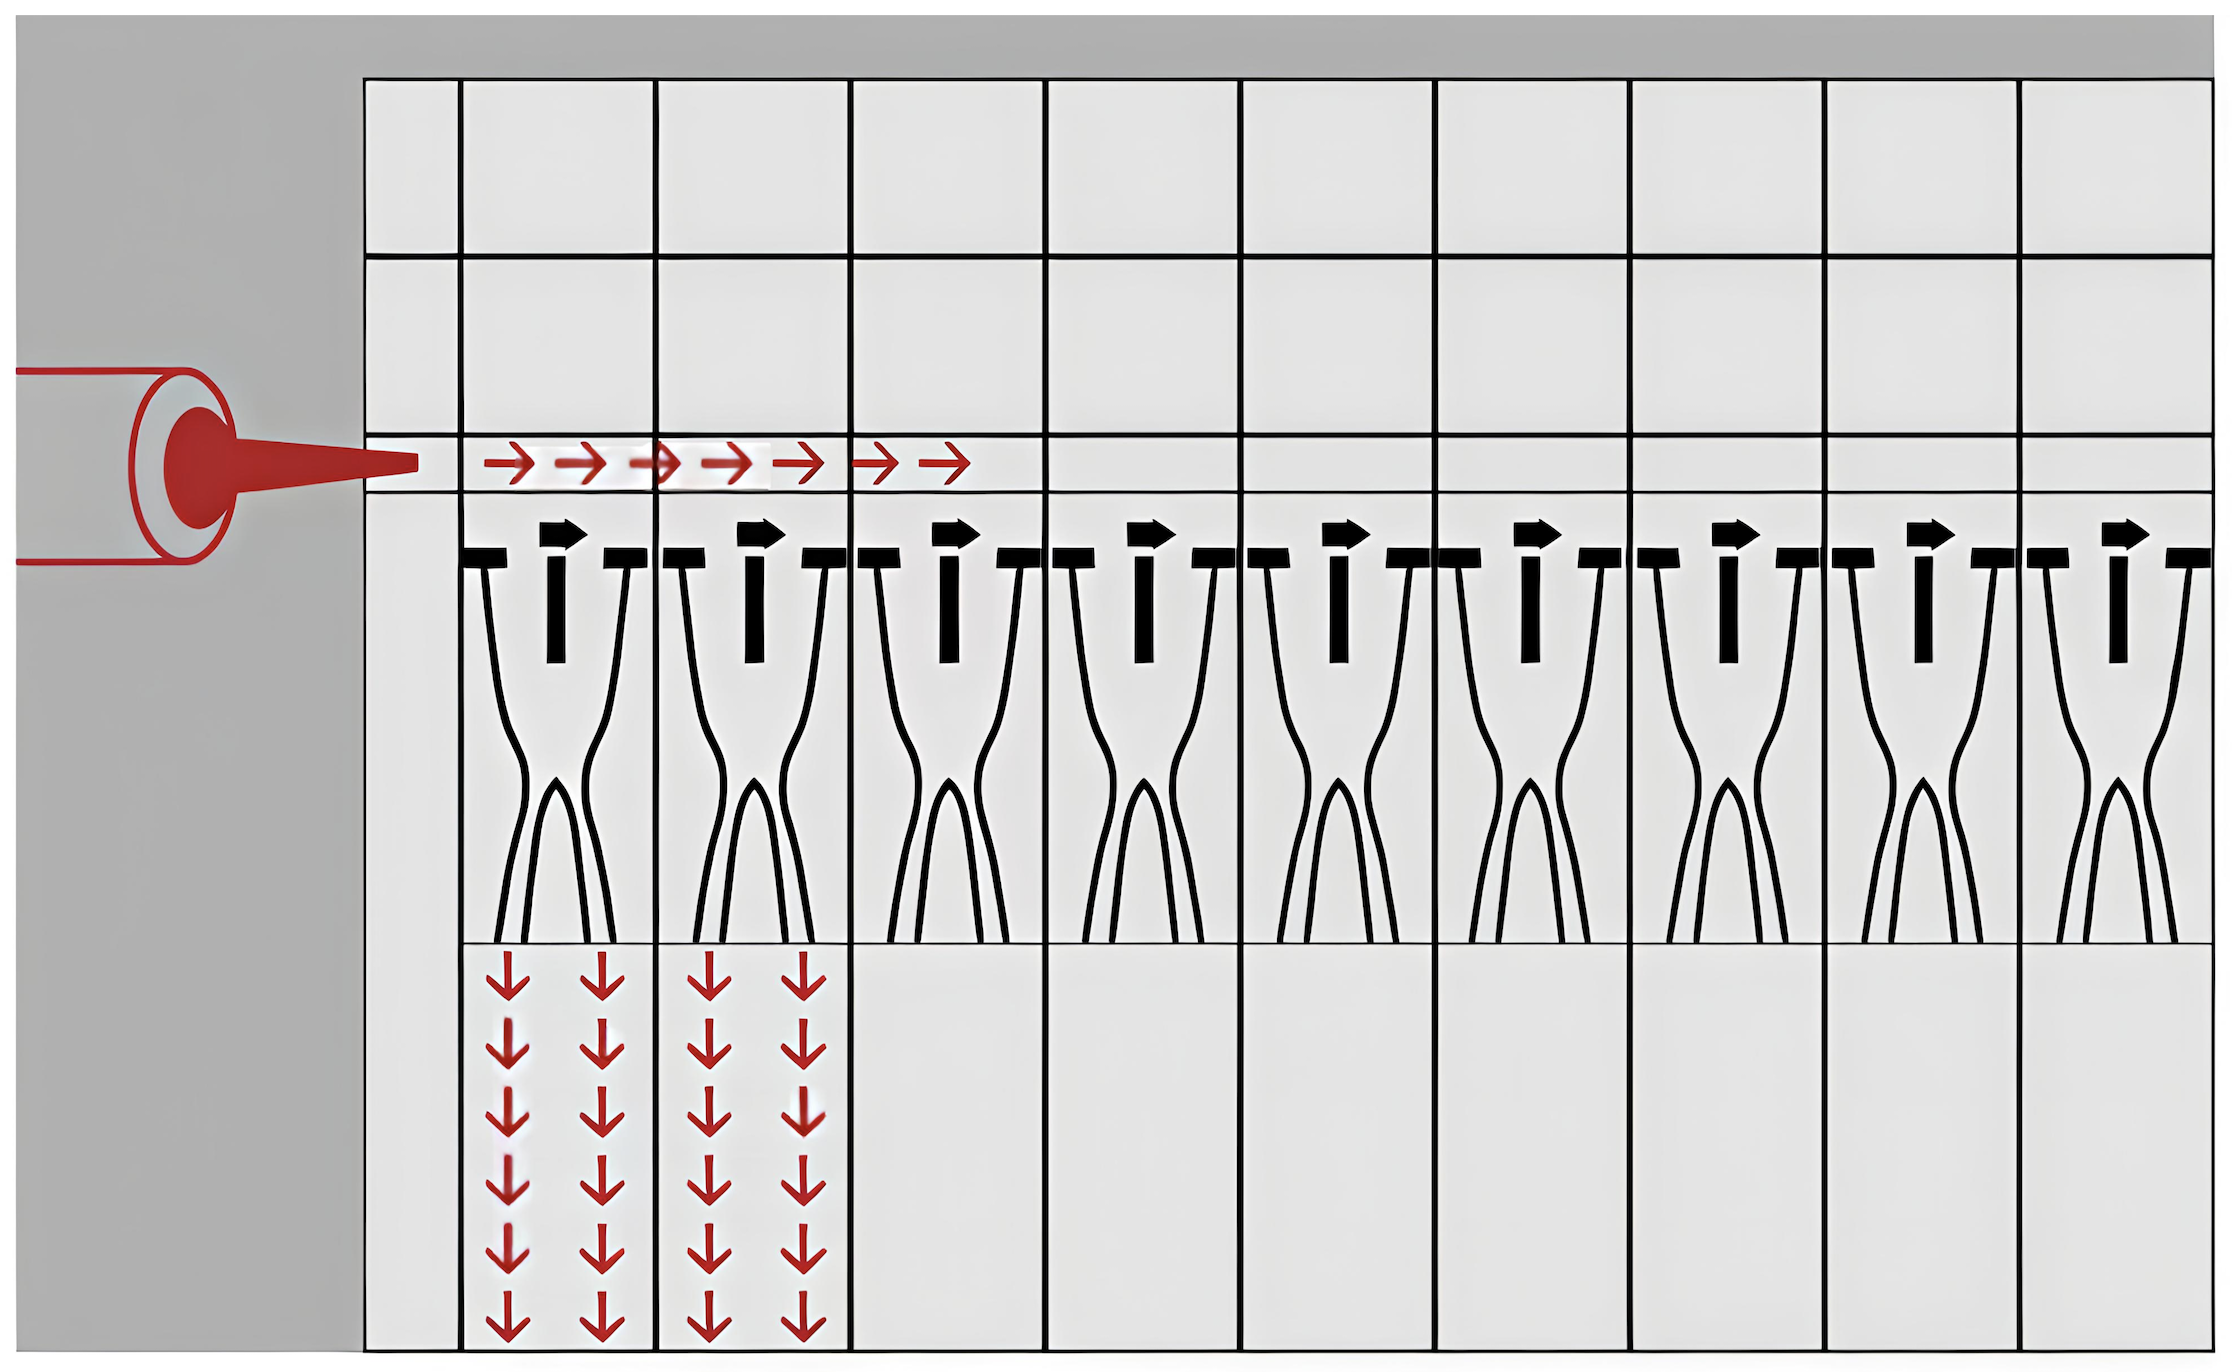
\includegraphics[width=0.65\textwidth]{figures/fig3_aircolumn_inflate.png}
    \caption{快递气柱充气工作原理示意图（单向阀自密封结构）}
    \label{fig:aircolumn_inflate}
\end{figure}

在样机验证阶段，采用车载 12\,V 微型充气泵进行充气操作，
充气时间约为 30$\sim$60\,s（视气柱总容积与泵的额定流量而定）。
充气完成后，充气阀自动密封，无需额外操作。

\subsection{气密性说明}
快递气柱采用PA复合薄膜热封工艺，气密性经过商业物流应用的充分验证。
在标准充气压力下，气柱可维持数小时至数天不发生明显漏气，
远超本系统单次使用的时间需求（约 5$\sim$10\,min）。
在实验阶段，气密保持时长测试结果详见第七章。



\section{本章小结}

本章完成了飞行雨伞充气骨架系统的设计。
系统以标准快递气柱为唯一结构承力件，配合 PLA 3D 打印节点
构成正方形模块化骨架，全程不使用刚性金属或碳纤维结构件。
骨架实物外框边长 870\,mm，对角旋翼轴距 1230\,mm，
TPU 伞面有效遮蔽面积约 0.608\,m$^2$。
充气展开采用车载微型充气泵，气密性满足单次使用需求。
上述结构参数将在第四章动力系统选型计算中作为输入条件使用。
      % 第三章 充气伞形结构设计
% ============================================================
% 第四章 动力系统设计与选型
% ============================================================

\chapter{动力系统设计与选型}

\section{整机质量预算}

动力系统选型的首要输入参数是整机起飞质量。
本系统对各部件质量进行系统梳理与预算，
所有数值以实物称重或厂商规格表数据为准，如表~\ref{tab:mass_budget}所示。

\begin{longtable}{llr}
    \caption{整机质量预算}
    \label{tab:mass_budget} \\

    % -------- 第一页表头 --------
    \toprule
    部件 & 型号/说明 & 质量 (g) \\
    \midrule
    \endfirsthead

    % -------- 续页表头 --------
    \multicolumn{3}{l}{\small 续表~\ref*{tab:mass_budget}} \\[2pt]
    \toprule
    部件 & 型号/说明 & 质量 (g) \\
    \midrule
    \endhead

    % -------- 每页底部（非末页）--------
    \midrule
    \multicolumn{3}{r}{\small 接下页} \\
    \endfoot

    % -------- 最后一页底部 --------
    \bottomrule
    \endlastfoot

    % -------- 表格内容 --------
    无刷电机 $\times 4$          & SIRIUS 2306.5-1850KV & 320 \\[3pt]
    电子调速器（ESC）$\times 4$  & —                    & 100 \\[3pt]
    桨叶 $\times 4$              & 51366 MCK v3         &  52 \\[3pt]
    飞行控制器                   & Pixhawk 6C           &  38 \\[3pt]
    GPS模块                      & —                    &  30 \\[3pt]
    遥控接收机                   & 乐迪 R9DS            &  15 \\[3pt]
    PLA节点结构件                & FDM 3D打印           & 600 \\[3pt]
    气柱骨架（全部）             & 快递气柱             & 150 \\[3pt]
    TPU伞面                      & TPU薄膜              & 150 \\[3pt]
    线缆与紧固件                 & —                    &  13 \\
    \midrule
    \textbf{整机合计}            & —                    & \textbf{1468} \\

\end{longtable}
电源延长线（14AWG，约150cm）对系统重心影响极小可忽略。
因此，整机起飞质量 $m = 1468$\,g（不含地面系留电源），
对应总重力：

\begin{equation}
    W = mg = 1.468 \times 9.81 = 14.40\,\text{N}
    \label{eq:weight}
\end{equation}

系统在悬停状态下所需的四旋翼总升力须满足 $T_{\text{total}} \geq W = 14.40$\,N。


\section{悬停升力需求与动量理论分析}

\subsection{悬停升力需求}

在静态悬停条件下，飞行器所需总升力等于整机重力，即：

\begin{equation}
    T_{\text{total}} = W = 14.40\,\text{N}
    \label{eq:hover_thrust}
\end{equation}

四旋翼对称布局下，单旋翼所需悬停升力为：

\begin{equation}
    T_{\text{single}} = \frac{T_{\text{total}}}{4} = \frac{14.40}{4} = 3.60\,\text{N} \approx 367\,\text{gf}
    \label{eq:single_thrust}
\end{equation}

\subsection{动量理论推导}

根据螺旋桨动量理论（Actuator Disk Theory），
旋翼在悬停状态下通过加速桨盘下方气流产生升力。
设桨盘面积为 $A$，气流诱导速度为 $v_i$，在无损理想情况下，推力与诱导速度的关系为：

\begin{equation}
    T = 2\rho A v_i^2
    \label{eq:momentum_theory}
\end{equation}

由此可解出悬停诱导速度：

\begin{equation}
    v_i = \sqrt{\frac{T}{2\rho A}}
    \label{eq:induced_velocity}
\end{equation}

本系统选用51366 MCK v3桨叶，桨盘直径 $D = 5.1$\,inch $= 129.5$\,mm，
对应桨盘面积：

\begin{equation}
    A = \pi \left(\frac{D}{2}\right)^2 = \pi \times (0.0648)^2 \approx 1.318 \times 10^{-2}\,\text{m}^2
    \label{eq:disk_area}
\end{equation}

取标准大气密度 $\rho = 1.225$\,kg/m$^3$，代入式~(\ref{eq:induced_velocity})：

\begin{equation}
    v_i = \sqrt{\frac{3.60}{2 \times 1.225 \times 1.318 \times 10^{-2}}} \approx 10.56\,\text{m/s}
    \label{eq:vi_result}
\end{equation}

\subsection{悬停功率估算}
根据动量理论，单旋翼的理想悬停诱导功率 $P_{i,\text{single}}$ 为推力与诱导速度的乘积：
\begin{equation}
    P_{i,\text{single}} = T_{\text{single}} v_i = 3.60 \times 10.56 \approx 38.02\,\text{W}
    \label{eq:ideal_power_single}
\end{equation}
四旋翼系统的总理想悬停功率为 $P_{i,\text{total}} = 4 \times 38.02 \approx 152.1\,\text{W}$。

在实际运行中，考虑到桨叶的叶型阻力、桨尖损失以及电机的机电转换损耗，
引入悬停效率系数（Figure of Merit, FM）进行修正。
结合所选电机与桨叶的测试经验数据，取综合效率系数 $\text{FM} = 0.70$，
则系统实际悬停总功率估算为：
\begin{equation}
    P_{\text{actual}} = \frac{P_{i,\text{total}}}{\text{FM}} = \frac{152.1}{0.70} \approx 217\,\text{W}
    \label{eq:actual_power}
\end{equation}
此功率值将作为后续续航时间估算的基准输入。


\section{电机与桨叶选型}

\subsection{选型依据}

基于上节计算，单旋翼悬停推力需求为367\,gf，
系统对电机选型提出以下约束条件：

\begin{itemize}
    \item 推力：在合理油门（$\leq 70\%$）下单电机推力须 $\geq 550$\,gf，
          以保证推重比 $\geq 1.5$；
    \item 效率：悬停工作点效率（g/W）尽量高，以延长续航时间；
    \item 重量：单电机质量 $\leq 100$\,g（四电机合计 $\leq 400$\,g）；
    \item 适配性：电机安装孔径与旋翼保护圈结构兼容。
\end{itemize}

\subsection{电机选型：SIRIUS 2306.5-1850KV}

本系统选用 \textbf{SIRIUS 2306.5-1850KV} 无刷电机，主要参数如表~\ref{tab:motor_spec}所示。

\begin{longtable}{ll}
    \caption{SIRIUS 2306.5-1850KV 电机主要参数}
    \label{tab:motor_spec} \\

    % -------- 第一页表头 --------
    \toprule
    参数 & 数值 \\
    \midrule
    \endfirsthead

    % -------- 续页表头 --------
    \multicolumn{2}{l}{\small 续表~\ref*{tab:motor_spec}} \\[2pt]
    \toprule
    参数 & 数值 \\
    \midrule
    \endhead

    % -------- 每页底部（非末页）--------
    \midrule
    \multicolumn{2}{r}{\small 接下页} \\
    \endfoot

    % -------- 最后一页底部 --------
    \bottomrule
    \endlastfoot

    % -------- 表格内容 --------
    定子尺寸     & 23\,mm $\times$ 6.5\,mm \\[3pt]
    KV值        & 1850\,rpm/V \\[3pt]
    推荐电池     & 4S $\sim$ 6S \\[3pt]
    单机质量     & 约 80\,g \\[3pt]
    最大连续电流  & 约 35\,A \\

\end{longtable}

% 电机图：左侧实物图 + 右侧工程图
SIRIUS~2306.5-1850KV 电机外观与尺寸如图~\ref{fig:motor}所示。

\begin{figure}[htbp]
    \centering
    \begin{subfigure}[b]{0.45\textwidth}
        \centering
        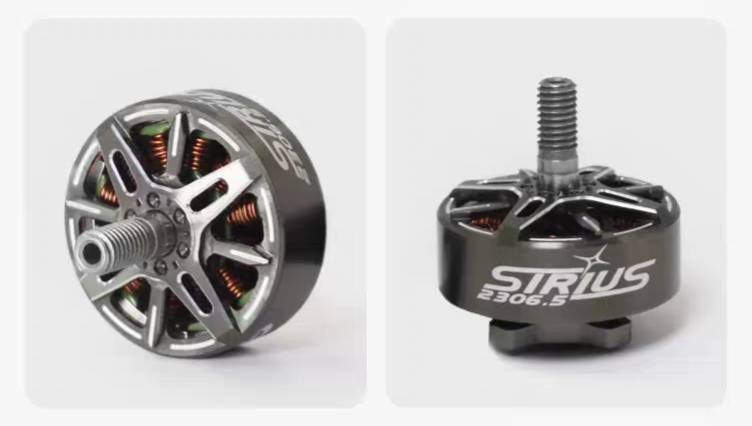
\includegraphics[width=\textwidth]{figures/fig4_2_motor_photo.jpeg}
        \caption{实物图}
        \label{fig:motor_photo}
    \end{subfigure}
    \hfill
    \begin{subfigure}[b]{0.45\textwidth}
        \centering
        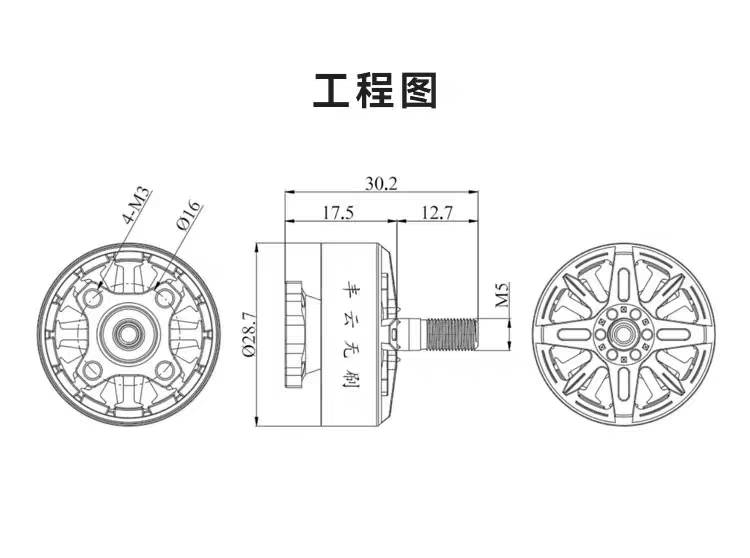
\includegraphics[width=\textwidth]{figures/fig4_2_motor_drawing.jpeg}
        \caption{工程图}
        \label{fig:motor_drawing}
    \end{subfigure}
    \caption{SIRIUS 2306.5-1850KV 无刷电机}
    \label{fig:motor}
\end{figure}

\subsection{桨叶选型：51366 MCK v3}
配套选用 \textbf{51366 MCK v3} 桨叶，直径5.1\,inch。
该桨叶实物如图~\ref{fig:propeller}所示。

\begin{figure}[htbp]
    \centering
    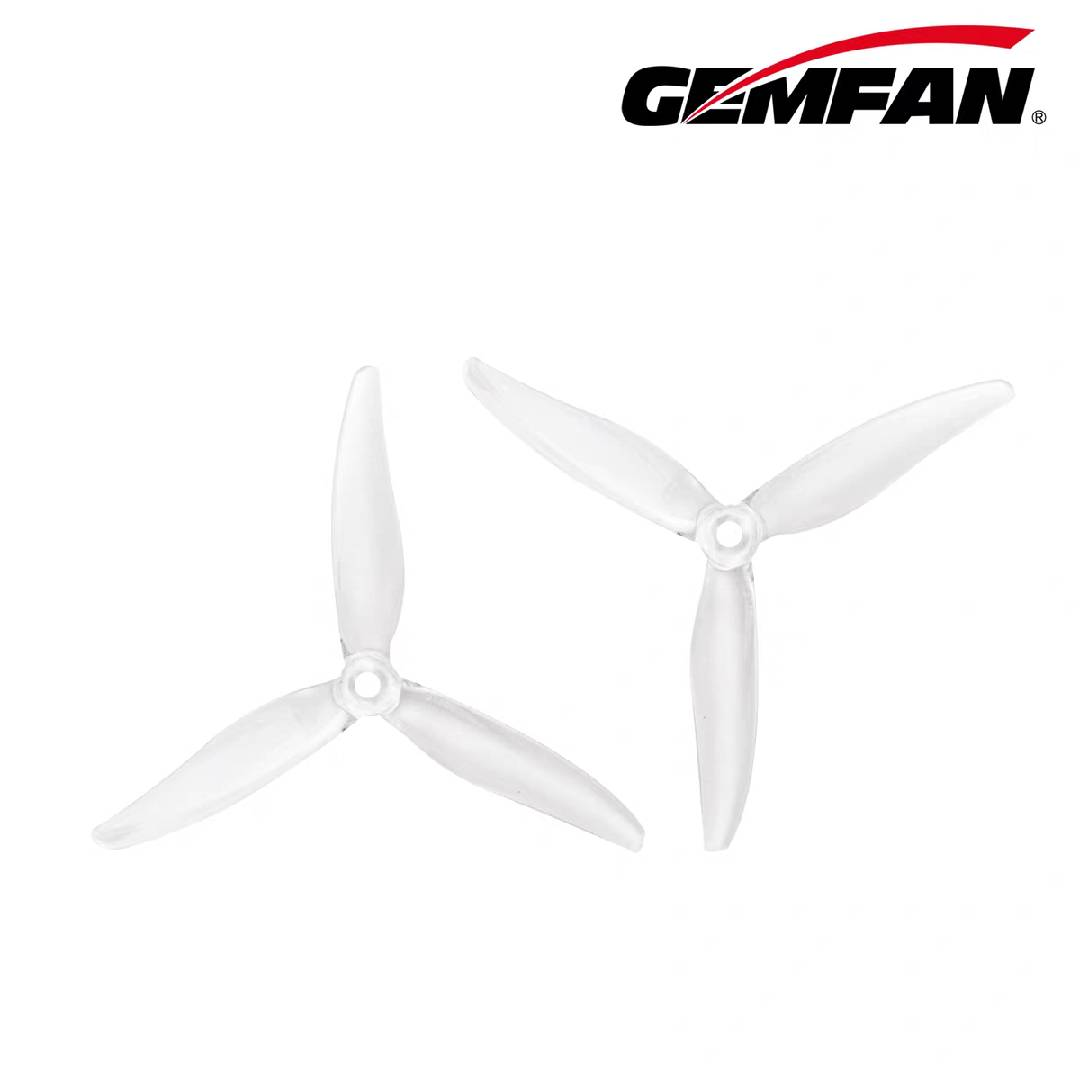
\includegraphics[width=0.30\textwidth]{figures/fig4_3_propeller_photo.jpeg}
    \caption{51366 MCK v3 桨叶实物图}
    \label{fig:propeller}
\end{figure}

在 6S（22.2\,V）电压下，配合 2100KV 级别电机使用时，
官方静态测试的典型推力-油门数据如表~\ref{tab:thrust_data}所示。

\begin{longtable}{lrrr}
    \caption{51366 MCK v3 桨叶推力测试数据（6S，四旋翼合计）}
    \label{tab:thrust_data} \\
    % -------- 第一页表头 --------
    \toprule
    油门（\%） & 单旋翼推力 (gf) & 四旋翼合计 (gf) & 推重比 \\
    \midrule
    \endfirsthead
    % -------- 续页表头 --------
    \multicolumn{4}{l}{\small 续表~\ref*{tab:thrust_data}} \\[2pt]
    \toprule
    油门（\%） & 单旋翼推力 (gf) & 四旋翼合计 (gf) & 推重比 \\
    \midrule
    \endhead
    % -------- 每页底部（非末页）--------
    \midrule
    \multicolumn{4}{r}{\small 接下页} \\
    \endfoot
    % -------- 最后一页底部 --------
    \bottomrule
    \endlastfoot
    % -------- 表格内容 --------
    30\%  &  205  &  820  & 0.56 \\[3pt]
    40\%  &  399  & 1596  & 1.09 \\[3pt]
    50\%  &  591  & 2364  & 1.61 \\[3pt]
    70\%  & 1113  & 4452  & 3.03 \\[3pt]
    90\%  & 1576  & 6304  & 4.29 \\
\end{longtable}


为了更直观地展示系统的动力冗余情况，绘制了如图~\ref{fig:thrust_curve}所示的推力-油门关系曲线。

\begin{figure}[htbp]
    \centering
    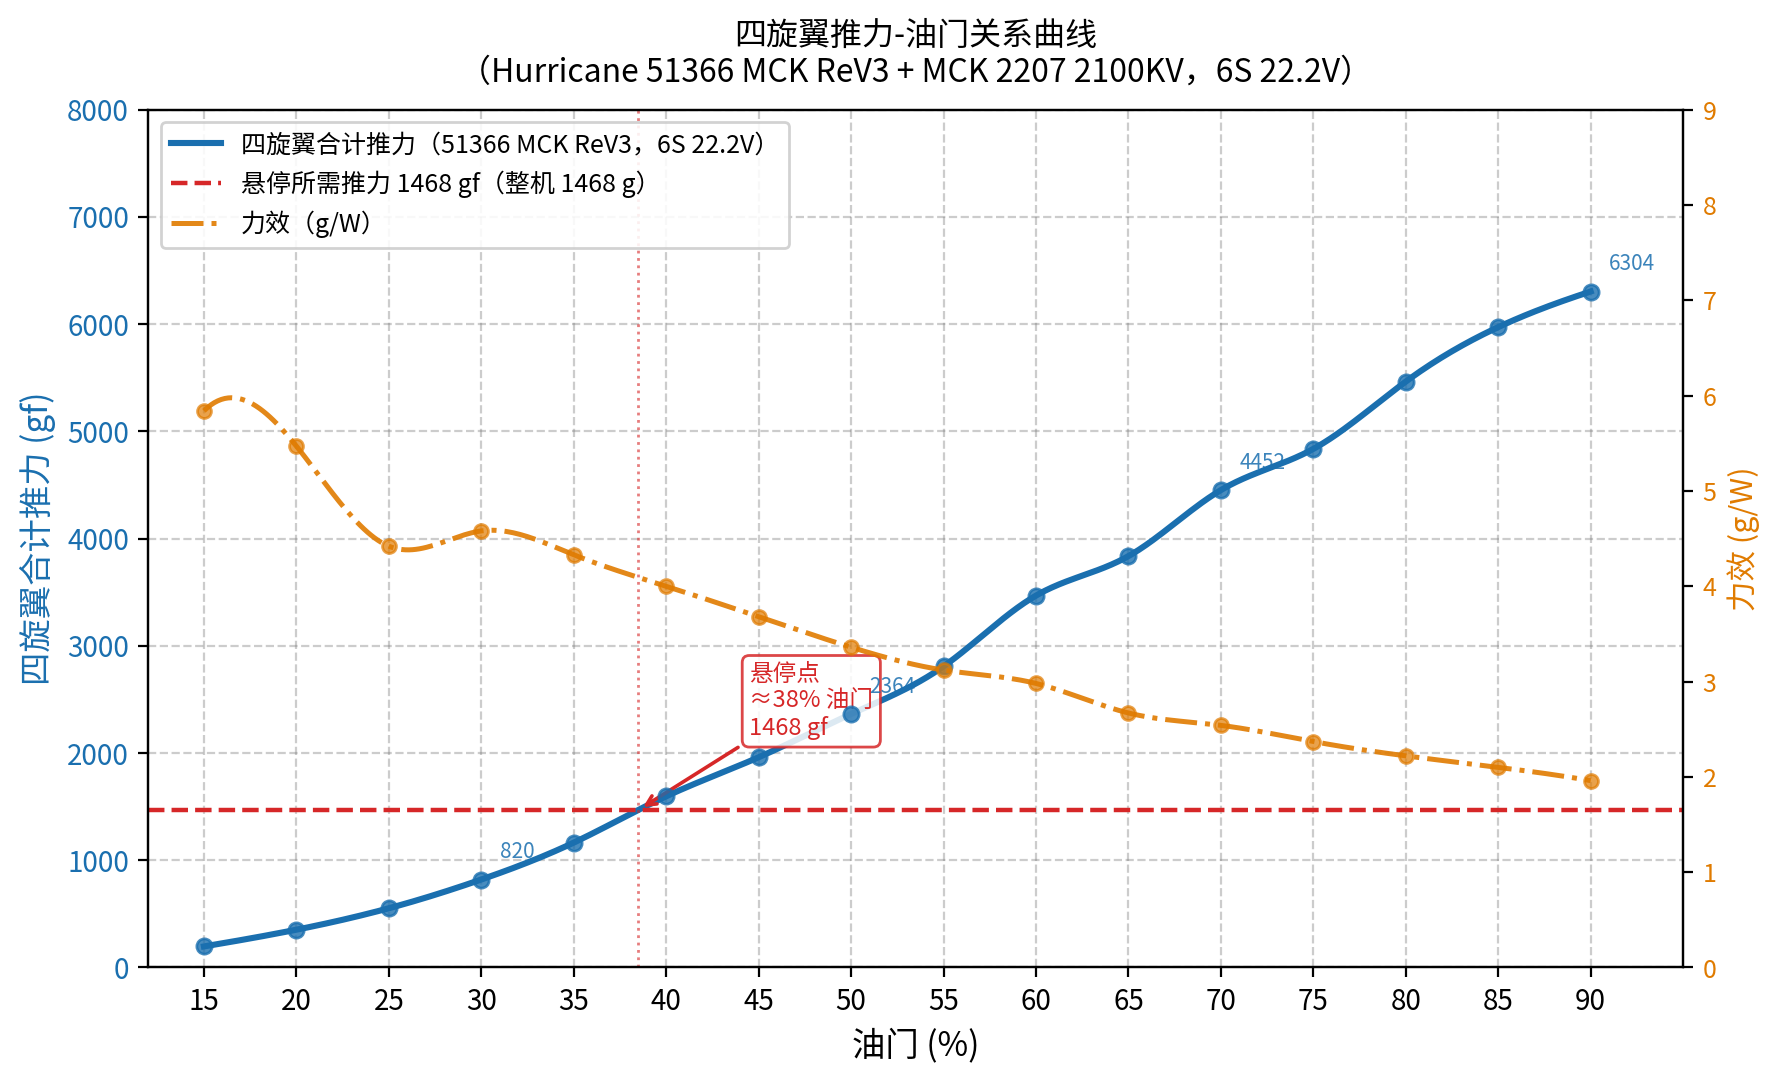
\includegraphics[width=0.85\textwidth]{figures/fig4_1_thrust_curve.png}
    \caption{四旋翼推力-油门关系曲线（6S 22.2V）}
    \label{fig:thrust_curve}
\end{figure}

由表~\ref{tab:thrust_data}及曲线图可知，系统悬停所需总推力 1468\,gf
约在 35\%$\sim$40\% 油门区间实现，\textbf{悬停工作油门约为 38\%}。
50\% 油门时推重比达 1.61，满足设计指标（$\geq 1.5$）要求，
动力储备充裕，具备良好的抗扰与机动能力。

% ----------------------------------------------------------

\section{气动阻力分析}
对于带有大面积遮蔽结构的飞行系统而言，气动载荷是影响飞行稳定性和动力消耗的关键因素。
本节将从垂直与侧向两个维度对系统的气动阻力进行分析。

\subsection{载荷位置对气动性能的影响}
多旋翼飞行器的气动性能受载荷位置影响显著。
Seth等人通过CFD仿真与实飞验证系统研究了载荷位于旋翼平面上方与下方两种配置的气动差异，
结果表明：载荷置于旋翼下方时，旋翼下洗流受到阻挡，
湍流强度显著增大，推力损失可达15\%$\sim$20\%，
俯仰/横滚姿态误差率约为20\%；
而当载荷置于旋翼上方时，下洗流路径畅通，
即使载荷覆盖面积达到桨盘面积的50\%，
推力损失可忽略不计，姿态误差率仅约0.1\%\cite{seth2023}。

本系统中，充气伞体主要结构位于旋翼平面\textbf{上方}，
与上述研究所验证的气动最优载荷位置完全一致，
从根本上避免了载荷对旋翼下洗流的干扰。
因此，以下分析更加关注侧向风载荷对系统姿态的影响。

\subsection{垂直方向气动分析}
充气伞面相对于旋翼桨盘位于上方，旋翼尾流在通过桨盘后向下加速。
伞面位于桨盘上方且面积相对于桨盘面积较大，
旋翼下洗流对伞面的直接影响可忽略不计。
在悬停工况下，伞面垂直方向气动阻力主要为静压差引起的上下面压差，
由于飞行速度接近零，此项气动力极小，对悬停推力需求的影响可忽略。

\subsection{侧向风载荷分析}
在侧风条件下，充气伞面及气柱骨架会受到侧向气动力。
根据第三章的几何设计，伞面呈拱形，具有约 12.8° 的平均倾角，其实际边长为 0.779\,m。
侧风吹袭时，系统的侧向有效迎风面积 $S_{\text{side}}$ 主要由伞面的倾斜投影决定：
\begin{equation}
    S_{\text{side}} = S_{\text{umbrella}} \times \sin(\alpha) = (0.779)^2 \times \sin(12.8^\circ) \approx 0.135\,\text{m}^2
\end{equation}
以侧风速度 $V_w = 3$\,m/s 为分析工况，采用平板阻力系数 $C_D \approx 1.3$，
系统受到的侧向气动阻力为：
\begin{equation}
    F_{\text{drag}} = \frac{1}{2}\rho V_w^2 C_D S_{\text{side}}
                    = \frac{1}{2} \times 1.225 \times 9 \times 1.3 \times 0.135
                    \approx 0.97\,\text{N} \approx 99\,\text{gf}
    \label{eq:drag}
\end{equation}
在 50\% 油门时，四旋翼合计推力约 2364\,gf。
侧向阻力（99\,gf）仅占50\%推力的约 4.2\%。
这表明伞面的 12.8° 倾角设计不仅有利于排水，还有效减小了侧向迎风面积，
使得系统具备极其充裕的侧向控制裕量，足以抵抗 3\,m/s 甚至更高级别的侧风扰动。

\section{续航时间估算}

基于式~(\ref{eq:actual_power})的悬停功率估算结果（$P \approx 217$\,W），
对两种供电形态下的续航时间进行理论估算。

\subsection{系留供电模式}

地面电源采用6S 10000\,mAh锂聚合物电池，
标称电压22.2\,V，储能约222\,Wh。
考虑电池放电效率、线缆损耗等实际因素（综合效率系数取0.65），
实际可用能量约144\,Wh，理论续航时间：

\begin{equation}
    t_{\text{tether}} = \frac{222 \times 0.65}{217} \times 60 \approx 40\,\text{min}
    \label{eq:endurance_tether}
\end{equation}

\subsection{自载电池模式}

机载电池采用6S 1500\,mAh，储能约33.3\,Wh，
理论续航时间：

\begin{equation}
    t_{\text{onboard}} = \frac{33.3 \times 0.65}{217} \times 60 \approx 6\,\text{min}
    \label{eq:endurance_onboard}
\end{equation}

自载模式主要用于功能验证与应急返航，其续航时间满足短时使用需求。
系留模式约40\,min的理论续航远超设计指标（$\geq 15$\,min），
在实际使用场景中具有充裕的使用时长。


\section{重心位置分析}

\subsection{重心高度估算}

以旋翼平面为基准面（$z = 0$），向上为正方向，
对各部件质心高度进行估算，如表~\ref{tab:cg_analysis}所示。

\begin{longtable}{lrrr}
    \caption{各部件质心高度与重心贡献}
    \label{tab:cg_analysis} \\

    % -------- 第一页表头 --------
    \toprule
    部件 & 质量 $m_i$ (g) & 质心高度 $z_i$ (mm) & $m_i z_i$ (g$\cdot$mm) \\
    \midrule
    \endfirsthead

    % -------- 续页表头 --------
    \multicolumn{4}{l}{\small 续表~\ref*{tab:cg_analysis}} \\[2pt]
    \toprule
    部件 & 质量 $m_i$ (g) & 质心高度 $z_i$ (mm) & $m_i z_i$ (g$\cdot$mm) \\
    \midrule
    \endhead

    % -------- 每页底部（非末页）--------
    \midrule
    \multicolumn{4}{r}{\small 接下页} \\
    \endfoot

    % -------- 最后一页底部 --------
    \bottomrule
    \endlastfoot

    % -------- 表格内容 --------
    电机 $\times 4$   & 320  &  0    &     0 \\[3pt]
    ESC $\times 4$    & 100  & $-$10 & $-$1000 \\[3pt]
    桨叶 $\times 4$   &  52  &  5    &   260 \\[3pt]
    Pixhawk 6C        &  38  &  40   &  1520 \\[3pt]
    GPS模块           &  30  &  50   &  1500 \\[3pt]
    接收机            &  15  &  35   &   525 \\[3pt]
    PLA节点结构件     & 600  &  5    &  3000 \\[3pt]
    气柱骨架          & 150  &  0    &     0 \\[3pt]
    TPU伞面          & 150  &  20   &  3000 \\[3pt]
    线缆与紧固件      &  13  &  0    &     0 \\
    \midrule
    \textbf{合计}     & \textbf{1468} & — & \textbf{8805} \\

\end{longtable}

整机质心高度：

\begin{equation}
    z_{\text{CG}} = \frac{\sum m_i z_i}{\sum m_i} = \frac{8805}{1468} \approx +6.0\,\text{mm}
    \label{eq:cg_height}
\end{equation}

整机质心位于旋翼平面\textbf{上方约6\,mm}处。

\subsection{重心偏高的影响分析}

质心位于旋翼平面以上，意味着系统在横向扰动下存在轻微的正反馈倾向，
即飞行器倾斜时重力分量会增大倾斜趋势。
然而，本系统质心偏高幅度仅约6\,mm，相对于1230\,mm的旋翼轴距而言极小（约0.5\%），
其对飞行稳定性的影响在正常PID控制范围内完全可以补偿，
无需进行配重调整或特殊控制策略设计。
飞控系统的PID参数整定策略将在第五章详细展开。


\section{本章小结}

本章完成了飞行雨伞系统动力系统的理论设计与选型。
整机起飞质量预算 1468\,g，对应悬停总升力需求 14.40\,N。
通过动量理论推导，悬停诱导速度约 10.56\,m/s，
理论悬停功率约 217\,W（含效率修正）。
选用 SIRIUS 2306.5-1850KV 电机配 51366 MCK v3 桨叶，
50\% 油门时推重比 2.32，悬停工作油门约 26\%$\sim$30\%。
系留模式理论续航约 40\,min，自载模式约 6\,min，均达到设计指标。
整机质心位于旋翼平面上方约 6\,mm，对飞行稳定性的影响可忽略。
上述计算结果将在第五章飞控参数整定中作为输入使用。

需要说明的是，以上质量数据为设计阶段的理论估算值；
第七章实测整机质量为 1683\,g，超出预算约 14.6\%，
具体原因见第七章 7.1.2 节分析。
           % 第四章 动力系统理论计算与选型
% ============================================================
% 第五章 飞行控制系统配置与调试
% ============================================================

\chapter{飞行控制系统配置与调试}

\section{多旋翼飞行动力学分析}

\subsection{坐标系定义}

本文采用右手坐标系进行动力学建模。
地理坐标系（惯性系）以起飞点为原点，$x$ 轴指向正北，$y$ 轴指向正东，$z$ 轴竖直向下。
机体坐标系固连于飞行器，原点位于质心，$x_b$ 轴指向机头方向，
$y_b$ 轴指向机身右侧，$z_b$ 轴向下。
姿态角采用欧拉角表示：滚转角 $\phi$、俯仰角 $\theta$、偏航角 $\psi$。

\subsection{六自由度运动方程}

多旋翼飞行器作为刚体，其运动由平动方程与转动方程共同描述。

\textbf{平动方程}（在惯性系下）：

\begin{equation}
    m\ddot{\boldsymbol{p}} = m\boldsymbol{g} + \boldsymbol{R} \cdot \boldsymbol{F}_b
    \label{eq:translation}
\end{equation}

其中 $\boldsymbol{p}$ 为位置向量，$\boldsymbol{R}$ 为从机体系到惯性系的旋转矩阵，
$\boldsymbol{F}_b = [0,\,0,\,-T_{\text{total}}]^T$ 为机体系下的合力（升力沿 $z_b$ 负方向）。

\textbf{转动方程}（在机体系下）：

\begin{equation}
    \boldsymbol{I}\dot{\boldsymbol{\omega}} + \boldsymbol{\omega} \times (\boldsymbol{I}\boldsymbol{\omega}) = \boldsymbol{\tau}
    \label{eq:rotation}
\end{equation}

其中 $\boldsymbol{I}$ 为转动惯量矩阵，$\boldsymbol{\omega} = [p,\,q,\,r]^T$ 为机体角速度，
$\boldsymbol{\tau} = [\tau_\phi,\,\tau_\theta,\,\tau_\psi]^T$ 为控制力矩。

对于正方形四旋翼X型布局，控制分配矩阵将四个电机推力
$[T_1,\,T_2,\,T_3,\,T_4]^T$ 映射为升力与三轴力矩：

\begin{equation}
    \begin{bmatrix} T_{\text{total}} \\ \tau_\phi \\ \tau_\theta \\ \tau_\psi \end{bmatrix}
    =
    \begin{bmatrix}
        1 &  1 &  1 &  1 \\
        L & -L & -L &  L \\
        L &  L & -L & -L \\
        k & -k &  k & -k
    \end{bmatrix}
    \begin{bmatrix} T_1 \\ T_2 \\ T_3 \\ T_4 \end{bmatrix}
    \label{eq:allocation}
\end{equation}

其中 $L = 0.435$\,m 为旋翼到机体坐标轴的力臂，$k$ 为电机反扭矩系数。

\subsection{充气伞形结构对飞行动力学的影响}

本系统相较于标准多旋翼飞行器，在动力学层面存在两项显著差异。

\subsubsection{转动惯量显著偏大}

以旋翼平面几何中心为转动基准，对系统各主要部件的转动惯量进行估算，
结果如表~\ref{tab:inertia}所示。

\begin{table}[htbp]
    \centering
    \caption{各部件转动惯量估算（绕 $x/y$ 轴）}
    \label{tab:inertia}
    \begin{tabular}{lrrr}
        \toprule
        部件              & 质量 (g) & 等效力臂 (mm) & $I_{xx}$ (kg$\cdot$m$^2$) \\
        \midrule
        旋翼单元 $\times 4$  & 492  & 435  & 0.093 \\
        PLA节点结构件        & 600  & 350  & 0.065 \\
        气柱骨架             & 150  & 均布  & 0.019 \\
        TPU伞面             & 150  & 均布  & 0.019 \\
        中心件（飞控等）      &  76  & $\approx 0$ & $\approx 0$ \\
        \midrule
        \textbf{合计}        & —    & —    & \textbf{0.196} \\
        \bottomrule
    \end{tabular}
\end{table}

本系统 $I_{xx} = I_{yy} \approx 0.196$\,kg$\cdot$m$^2$，
$I_{zz} \approx 0.393$\,kg$\cdot$m$^2$。
相比典型450\,mm轴距四旋翼（$I_{xx} \approx 0.012$\,kg$\cdot$m$^2$），
本系统转动惯量\textbf{约为标准四旋翼的16倍}，
主要来源于1230\,mm超大轴距与大面积骨架的质量分布。

转动惯量大意味着：相同控制力矩下角加速度更小，姿态响应较慢；
但同时在低速悬停时对小扰动的角加速度响应更迟钝，
飞行器表现出更好的姿态自然稳定性。
在PID参数整定时，大转动惯量要求\textbf{显著降低比例增益P}，
否则控制力矩相对于惯量过强，易引发姿态震荡。

\subsubsection{重心略高于旋翼平面}

由第四章计算，整机质心位于旋翼平面上方约6\,mm处。
该偏高幅度相对于1230\,mm旋翼轴距仅约0.5\%，
对飞行稳定性影响极小，在正常PID控制范围内可完全补偿，
无需进行配重调整或特殊控制策略设计。


\section{Pixhawk 6C嵌入式飞控系统}

\subsection{硬件架构}

本系统选用 \textbf{Pixhawk 6C} 开源飞控硬件平台。
Pixhawk 6C搭载STM32H753主处理器（480\,MHz）与STM32F100协处理器，
集成三轴加速度计与陀螺仪（ICM-42688-P）、
气压计（MS5611）、磁罗盘接口等传感器，
运行 \textbf{NuttX实时操作系统}与 \textbf{PX4飞控固件}。
主要硬件参数如表~\ref{tab:pixhawk_spec}所示。

\begin{table}[htbp]
    \centering
    \caption{Pixhawk 6C 主要硬件参数}
    \label{tab:pixhawk_spec}
    \begin{tabular}{ll}
        \toprule
        参数           & 规格 \\
        \midrule
        主处理器        & STM32H753（480\,MHz，2\,MB Flash） \\
        加速度计/陀螺仪 & ICM-42688-P \\
        气压计          & MS5611 \\
        工作电压        & 4.75$\sim$5.25\,V \\
        自重            & 约38\,g \\
        PWM输出         & 8路 \\
        通信接口        & UART $\times$6，I$^2$C $\times$2，SPI $\times$3 \\
        \bottomrule
    \end{tabular}
\end{table}

\subsection{PX4控制回路架构}

PX4固件实现了完整的多旋翼飞行控制回路，采用\textbf{内外环级联控制}结构：

\begin{itemize}
    \item \textbf{姿态控制回路（内环）}：以IMU测量的角速度与姿态角为反馈，
          通过PID控制器输出控制力矩指令，再经控制分配矩阵转换为各电机PWM指令。
          姿态回路运行频率约250$\sim$1000\,Hz。
    \item \textbf{位置控制回路（外环）}：以GPS/气压计测量的位置与速度为反馈，
          输出期望姿态角指令给姿态回路。位置回路运行频率约50\,Hz。
\end{itemize}

本系统在验证阶段主要使用\textbf{姿态稳定模式（Stabilize）}
与\textbf{定高模式（Altitude Hold）}，
通过乐迪AT9S Pro遥控器进行手动控制，不涉及全自主飞行。

% ----------------------------------------------------------
% [图片占位 Fig.5.1] ★推荐制作★
% 内容：PX4双环控制回路框图
%   外环（位置控制）→ 期望姿态角 → 内环（姿态控制）→ 电机PWM → 飞行器
%   可参考PX4官方文档的控制架构图，手绘或用draw.io简化绘制
% \begin{figure}[htbp]
%     \centering
%     \includegraphics[width=0.80\textwidth]{figures/fig5_1_px4_control_loop.png}
%     \caption{PX4双环级联控制回路架构}
%     \label{fig:px4_loop}
% \end{figure}
% ----------------------------------------------------------

\subsection{传感器配置与校准}

飞控系统集成以下传感器，均通过QGroundControl（QGC）地面站完成校准：

\begin{itemize}
    \item \textbf{IMU}：六点加速度计校准，消除零偏与比例误差；陀螺仪上电自动校准；
    \item \textbf{磁罗盘}：椭球拟合旋转校准，消除硬铁/软铁干扰；
    \item \textbf{气压计}：自动温度补偿，用于定高模式高度保持；
    \item \textbf{遥控器}：通道映射与摇杆行程校准，油门曲线线性化设置。
\end{itemize}

由于本系统骨架为气柱薄膜材料（无铁磁性），对磁罗盘的干扰极小，
磁罗盘校准结果良好。四个ESC通过物理隔离（远离飞控安装位）
有效抑制无刷电机工作时的电磁干扰。


\section{针对充气伞形结构的PID参数整定}

\subsection{整定难点分析}

本系统在PID参数整定方面面临以下有别于标准多旋翼的特殊挑战：

\begin{itemize}
    \item \textbf{大转动惯量导致的响应迟滞}：
          如5.1节分析，本系统转动惯量约为同质量标准四旋翼的16倍。
          若照搬标准四旋翼PID参数，比例项P过大会导致控制力矩远超实际需求，
          引发姿态过冲甚至持续震荡；初始整定时须显著降低P增益。

    \item \textbf{伞面气动阻尼的影响}：
          充气伞面的大面积对空气运动产生显著的气动阻尼，
          使系统在横向扰动下具有较大的自然衰减效果，
          有利于减少超调，但可能造成姿态响应不灵敏，
          需适当补偿微分项D。

    \item \textbf{悬停油门预设}：
          本系统悬停油门约26\%$\sim$30\%，
          远低于PX4默认的50\%悬停油门预设，
          需在飞行前通过参数 \texttt{MPC\_THR\_HOVER} 进行修正，
          否则飞控在切换定高模式时会产生较大的高度跳变。
\end{itemize}

\subsection{初始PID参数设置}

鉴于本系统大转动惯量特性，初始参数在PX4默认值基础上进行调整，
如表~\ref{tab:pid_params}所示。

\begin{table}[htbp]
    \centering
    \caption{PID参数初始设定值（相对PX4默认值）}
    \label{tab:pid_params}
    \begin{tabular}{lrrl}
        \toprule
        参数名称             & PX4默认值 & 初始设定值 & 调整依据 \\
        \midrule
        \texttt{MC\_ROLLRATE\_P}   & 0.150 & 0.050 & 大转动惯量，P降至默认值1/3 \\
        \texttt{MC\_ROLLRATE\_I}   & 0.100 & 0.050 & 保留I项消除稳态误差 \\
        \texttt{MC\_ROLLRATE\_D}   & 0.003 & 0.008 & D适当增大补偿气动阻尼 \\
        \texttt{MC\_PITCHRATE\_P}  & 0.150 & 0.050 & 同Roll轴 \\
        \texttt{MC\_PITCHRATE\_I}  & 0.100 & 0.050 & 同Roll轴 \\
        \texttt{MC\_PITCHRATE\_D}  & 0.003 & 0.008 & 同Roll轴 \\
        \texttt{MC\_YAWRATE\_P}    & 0.200 & 0.080 & 偏航惯量更大，P进一步降低 \\
        \texttt{MC\_YAWRATE\_I}    & 0.100 & 0.040 & — \\
        \texttt{MPC\_THR\_HOVER}   & 0.500 & 0.280 & 悬停油门约26\%$\sim$30\% \\
        \bottomrule
    \end{tabular}
\end{table}

\subsection{整定流程}

参数整定依照以下步骤进行，全程使用QGC地面站实时监控飞行状态与日志：

\begin{description}
    \item[第一步：机型配置]
        在QGC中选择机型为"Generic Quadrotor X"，
        按PX4标准X型四旋翼顺序连接电机：
        1号（右前，逆时针）、2号（左后，逆时针）、
        3号（左前，顺时针）、4号（右后，顺时针）。

    \item[第二步：传感器校准]
        依次完成加速度计六点校准、磁罗盘旋转校准、
        遥控器通道校准与油门曲线线性化设置。

    \item[第三步：参数预设]
        按表~\ref{tab:pid_params}输入初始PID参数，
        同时设置 \texttt{MPC\_THR\_HOVER = 0.28}，
        \texttt{MOT\_SPIN\_MIN = 0.05}（最低电机转速，防止低油门停转）。

    \item[第四步：绑绳悬停测试]
        用四根软绳（约1\,m长）从四个方向固定飞行器，
        推油门至悬停点，观察飞行器姿态稳定性与震荡情况。
        若出现明显的Roll/Pitch震荡，继续降低对应轴的P增益；
        若响应过于迟钝，适当增大D增益。

    \item[第五步：自由悬停精调]
        解除绑绳，在空旷场地进行自由悬停测试，
        根据实际姿态响应逐步微调P、I、D参数至稳定悬停状态。
        调整原则：P决定响应速度，I消除稳态漂移，D抑制过冲。
\end{description}

% ----------------------------------------------------------
% [图片占位 Fig.5.2] ★推荐制作★
% 内容：QGC地面站参数配置界面截图
%   截图内容：Parameters页面，显示MC_ROLLRATE_P等参数输入框
%   或：飞行日志中Roll/Pitch角度曲线，显示调参前后对比
%   用QGC软件截图即可，无需额外绘制
% \begin{figure}[htbp]
%     \centering
%     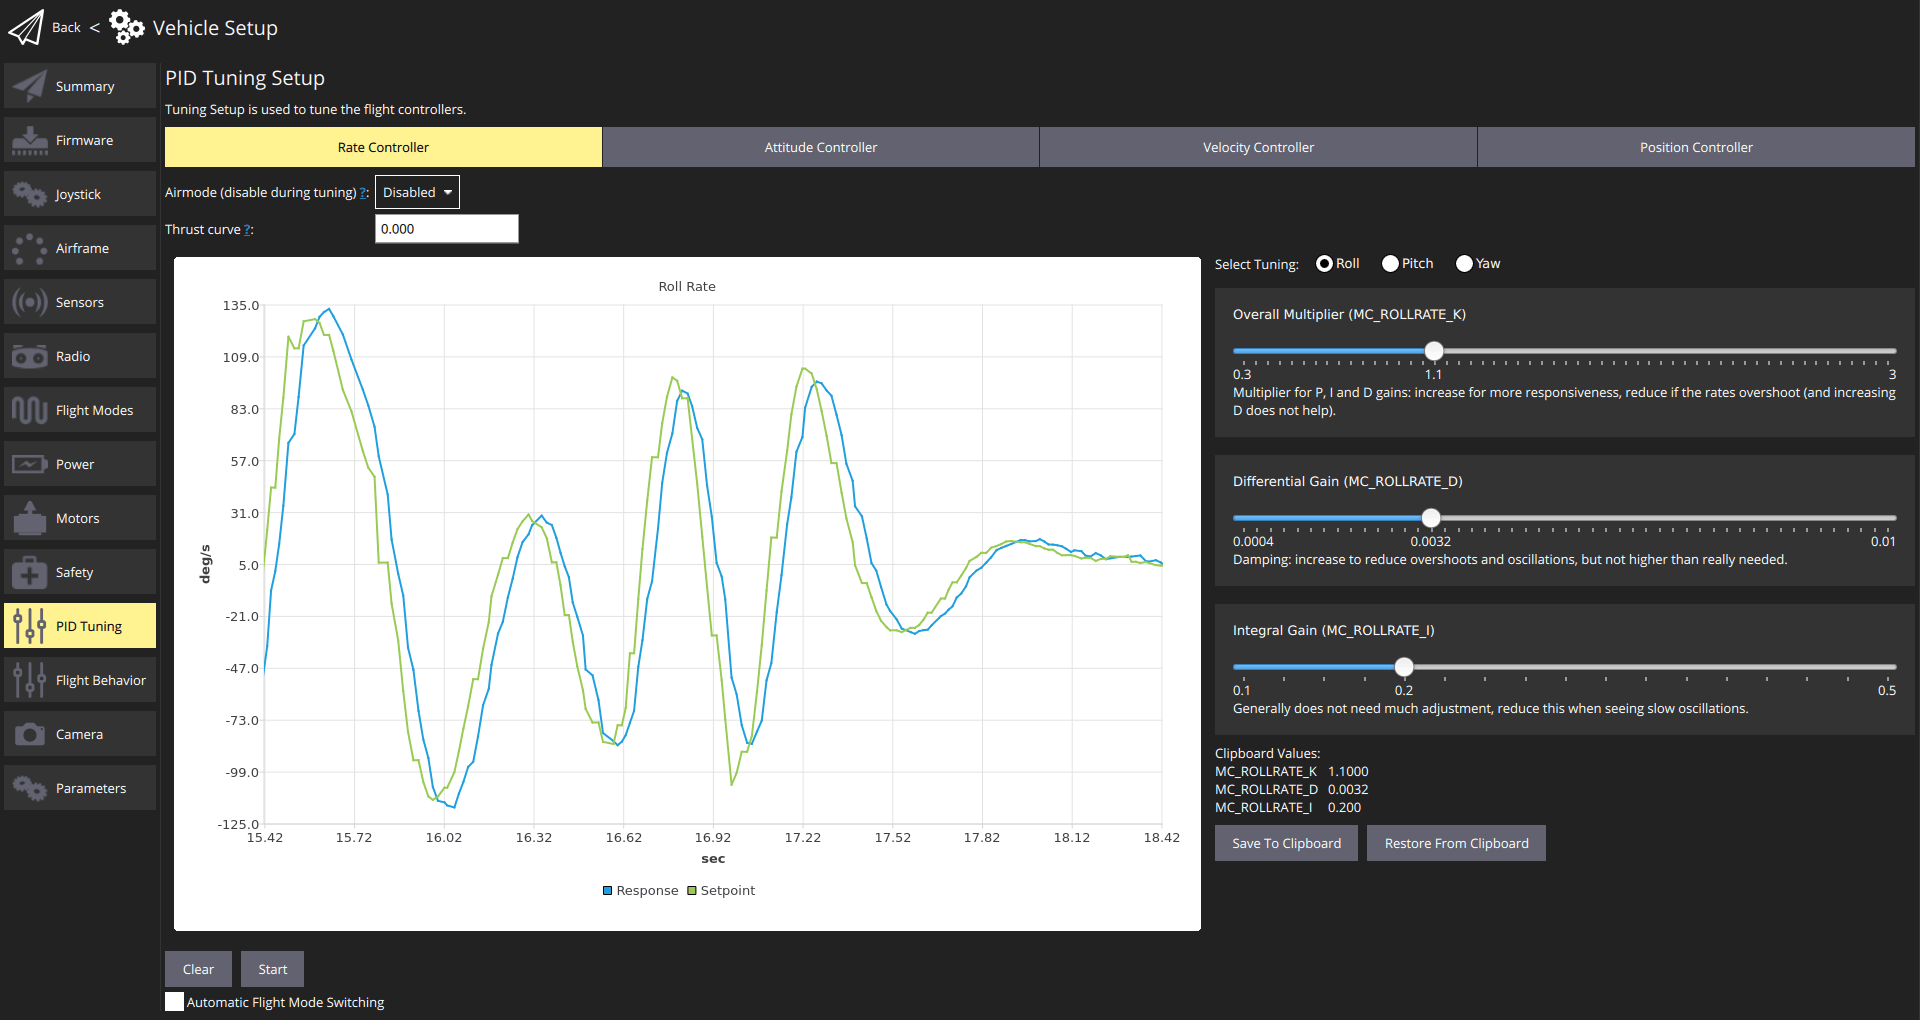
\includegraphics[width=0.75\textwidth]{figures/fig5_2_qgc_params.png}
%     \caption{QGroundControl地面站PID参数配置界面}
%     \label{fig:qgc_params}
% \end{figure}
% ----------------------------------------------------------


\section{通信链路配置}

\subsection{遥控链路}

本系统使用\textbf{乐迪AT9S Pro}遥控器（9通道，2.4\,GHz FHSS跳频扩频技术），
配套R9DS接收机通过SBUS协议与Pixhawk 6C连接。
控制信号链路如下：

\begin{center}
AT9S Pro遥控器
$\xrightarrow{\text{2.4\,GHz FHSS}}$
R9DS接收机
$\xrightarrow{\text{SBUS}}$
Pixhawk 6C
$\xrightarrow{\text{PWM/DSHOT}}$
ESC $\times 4$
$\rightarrow$
电机 $\times 4$
\end{center}

遥控器通道分配如下：
通道1（副翼/Roll）、通道2（升降/Pitch）、
通道3（油门/Throttle）、通道4（方向/Yaw）、
通道5（飞行模式切换）、通道6（紧急锁定/Kill Switch）。

\subsection{失控保护配置}

AT9S Pro支持失控保护（Failsafe）功能：
当遥控信号持续丢失超过0.5\,s时，
飞控自动执行预设的失控保护动作。
结合本系统最大飞行高度不超过2\,m的工作约束，
失控保护动作设置为\textbf{原地降落（Land）}模式，
确保在任何情况下飞行器均能安全落地，不会对周围人员造成安全威胁。


\section{本章小结}

本章完成了飞行雨伞系统飞行控制系统的配置与调试方案设计。
通过建立多旋翼六自由度动力学模型，分析了充气伞形结构对飞行动力学的两项特殊影响：
转动惯量约为标准四旋翼的16倍（$I_{xx} \approx 0.196$\,kg$\cdot$m$^2$），
以及质心偏高约6\,mm。
基于Pixhawk 6C飞控平台与PX4固件，完成了传感器校准、
电机接线配置与飞行模式设置。
针对大转动惯量特性，制定了系统性的PID参数初始整定策略，
将Roll/Pitch比例增益降至PX4默认值的1/3，
并提出了绑绳悬停→自由悬停的渐进式调试流程，
为飞行验证阶段提供了完整的调试方案。         % 第五章 嵌入式飞行控制系统
% ============================================================
% 第六章 系统集成与车载使用场景设计
% ============================================================

\chapter{系统集成与车载使用场景设计}

\section{系统集成概述}

\subsection{系统总体架构}

飞行雨伞系统由四个相互独立又协同工作的子系统构成，
如表~\ref{tab:subsystem_overview}所示。

\begin{longtable}{p{3.2cm} p{5.0cm} p{5.5cm}}
    \caption{飞行雨伞系统子系统构成}
    \label{tab:subsystem_overview} \\

    % -------- 第一页表头 --------
    \toprule
    子系统 & 核心组件 & 功能定位 \\
    \midrule
    \endfirsthead

    % -------- 续页表头 --------
    \multicolumn{3}{l}{\small 续表~\ref*{tab:subsystem_overview}} \\[2pt]
    \toprule
    子系统 & 核心组件 & 功能定位 \\
    \midrule
    \endhead

    % -------- 每页底部（非末页）--------
    \midrule
    \multicolumn{3}{r}{\small 接下页} \\
    \endfoot

    % -------- 最后一页底部 --------
    \bottomrule
    \endlastfoot

    % -------- 表格内容 --------
    充气伞体系统
        & 气柱骨架、TPU伞面、PLA节点、充气阀
        & 形态重构载体，实现收纳$\leftrightarrow$飞行形态切换 \\[6pt]
    多旋翼动力系统
        & 电机$\times$4、ESC$\times$4、桨叶$\times$4、电池
        & 提供飞行升力，实现姿态与位置控制 \\[6pt]
    嵌入式飞行控制系统
        & Pixhawk 6C、IMU、气压计、GPS
        & 传感器融合、姿态估计与控制律解算 \\[6pt]
    车载平台系统
        & 车载充气泵、遥控器、地面电源、收纳袋
        & 提供充气、控制与能源支持，实现车载集成 \\


\end{longtable}
\FloatBarrier 
飞行雨伞系统的整机集成（收纳）形态如图~\ref{fig:drone_cad}所示，
四个旋翼单元通过气柱骨架与正方形中心框架连接，
飞控（绿色）安装于中心框架顶部，整体结构紧凑对称。

\begin{figure}[htbp]
    \centering
    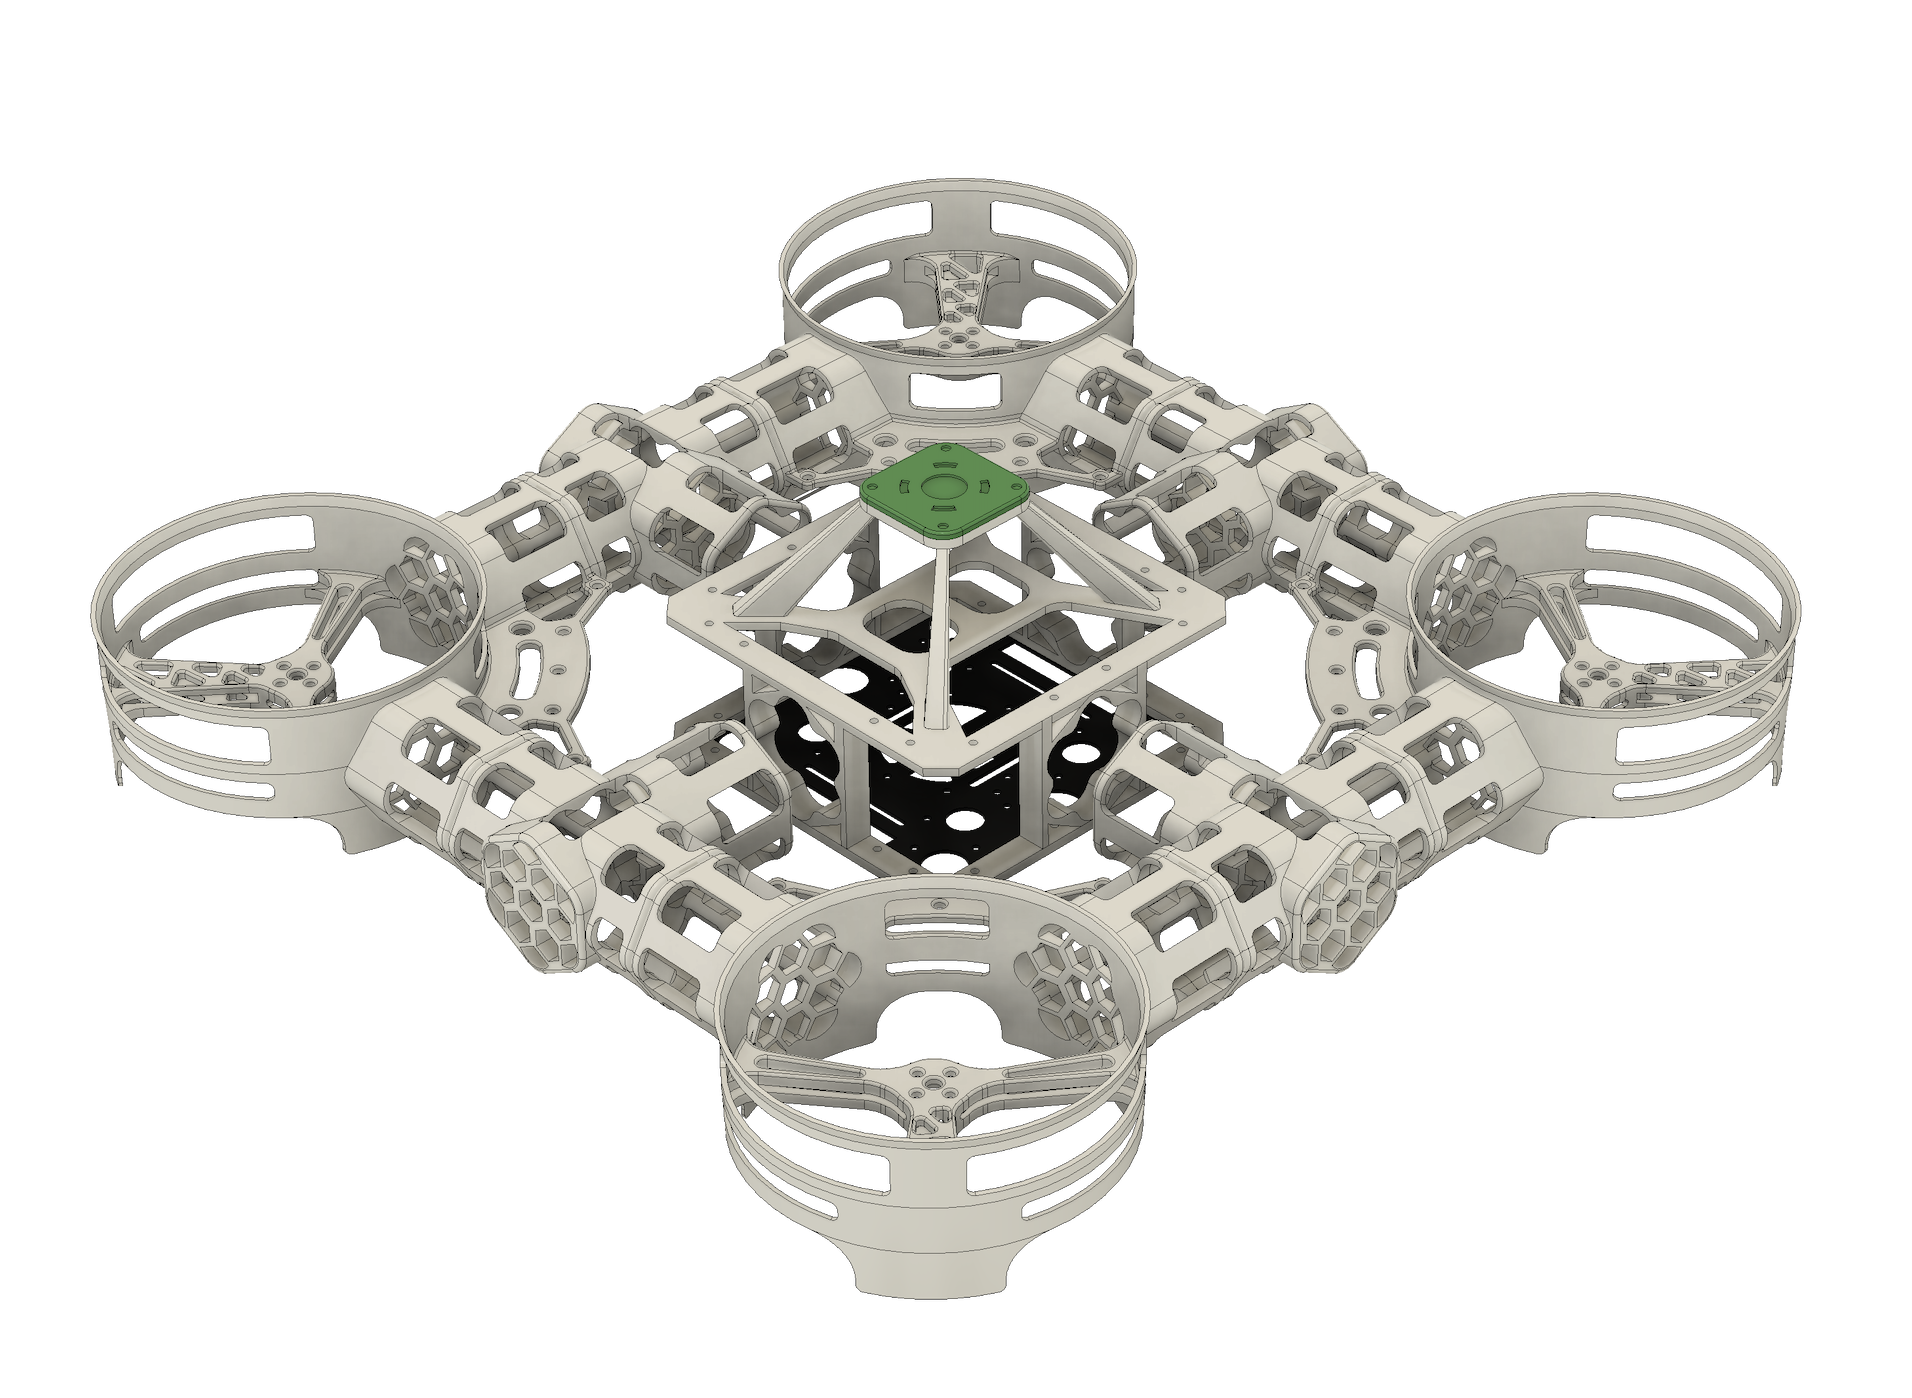
\includegraphics[width=0.35\textwidth]{figures/fig6_drone_cad.png}
    \caption{飞行雨伞系统收纳态CAD渲染图}
    \label{fig:drone_cad}
\end{figure}
\FloatBarrier

\subsection{电子系统集成架构}

动力飞行子系统的电子集成采用标准多旋翼架构，信号与电源流如下：

\textbf{遥控信号链路}：乐迪AT9S Pro（9通道，2.4\,GHz FHSS）
$\rightarrow$ R9DS接收机 $\rightarrow$ Pixhawk 6C（SBUS协议）

\textbf{控制输出链路}：Pixhawk 6C $\rightarrow$ ESC$\times$4（PWM协议）
$\rightarrow$ 无刷电机$\times$4

\textbf{传感回路}：IMU（内置）+ 气压计（内置）+ GPS（外置，UART接口）
$\rightarrow$ Pixhawk 6C状态估计器

飞控安装于骨架中心平台，GPS模块固定于飞控上方伞面固定架，
远离电机以减少电磁干扰。
四个ESC沿骨架气柱布线，通过扎带固定于对应气柱外侧，
保持整体布局的重心对称性。


\section{收纳态设计}

\subsection{收纳形态特征}

充气结构子系统的核心设计价值之一，在于实现从"飞行器"到"随身携带物品"的形态降维。
当气柱骨架完全排气后，整个系统折叠为厚度约3$\sim$5\,cm的扁平形态，
平面尺寸与一台笔记本电脑相当。

如图~\ref{fig:concept_render}所示，收纳态的飞行雨伞外形圆润紧凑，
整机起飞质量约 1.68\,kg（含机载电池），可单手持握，或置于专属收纳袋中存放于车辆后备箱、
座椅背后等空间。
这一形态特征从根本上消除了传统无人机"体积庞大、不便携带"的使用痛点，
使飞行雨伞真正具备随车常备的可行性。


\begin{figure}[htbp]
    \centering
    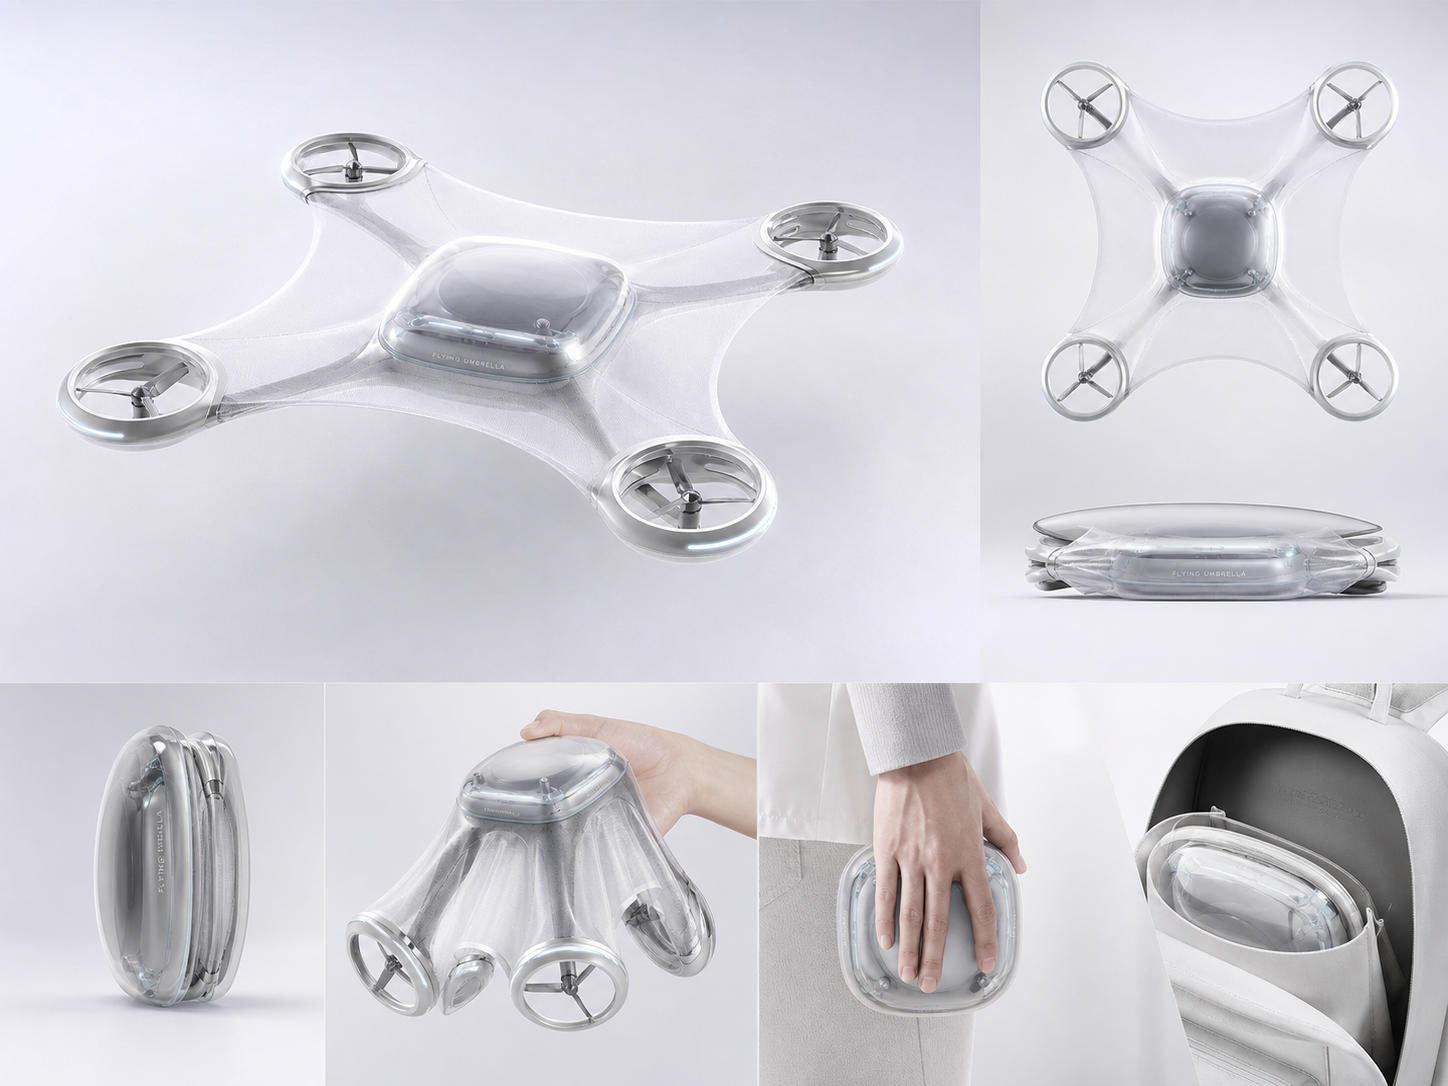
\includegraphics[width=0.75\textwidth]{figures/fig6_1_concept_render.png}
    \caption{飞行雨伞系统收纳态与飞行态概念效果图}
    \label{fig:concept_render}
\end{figure}
\FloatBarrier 

\subsection{收纳操作流程}

从飞行态到收纳态的转换操作步骤如下：

\begin{enumerate}
    \item 飞行雨伞完成飞行任务，操控降落至地面；
    \item 关闭电机，确认系统安全停机；
    \item 打开充气阀放气口，气柱在大气压差作用下自然排气；
    \item 配合手动辅助按压加速排气过程（约10$\sim$20\,s完成）；
    \item 将排气后的扁平结构折叠收纳，放入收纳袋归位。
\end{enumerate}

整个收纳操作无需工具，由单人即可完成，预计操作时间不超过60\,s。


\section{车载部署方案设计}

\subsection{车载存放方案}

飞行雨伞的车载存放依托新能源汽车后备箱空间实现。
收纳态系统置于专属收纳袋，与车载充气泵、遥控器等配件一同存放于后备箱，
不占用乘坐空间，亦不影响日常用车。

收纳袋设计需满足以下要求：防水材质（应对雨天取用场景）；
有一定保护衬垫（防止气柱在车辆行驶振动中磨损）；
开合方便（单手可操作）。
收纳袋通过魔术贴或弹性绑带固定于后备箱侧壁或底板，
防止车辆行驶时滑移，适配市售大多数SUV和轿车车型，
无需对车辆进行任何改造。

\subsection{充气展开方案}

车载充气泵采用12\,V直流微型充气泵，
通过车辆点烟器接口或12\,V车载电源接口供电，无需额外电源设备。
充气时，将充气泵气嘴对接飞行雨伞骨架上的充气阀接口，开启充气泵即可。

充气过程中，骨架气柱和伞面气柱依次充气，
系统从扁平收纳态逐渐展开为正方形飞行形态。
充气完成时间约30$\sim$60\,s（取决于充气泵额定流量）。
充气完成后，充气阀自动密封，断开充气泵接口即可准备起飞。

\subsection{起降平台设计考量}

在当前样机阶段，飞行雨伞的起飞与降落地点为车辆附近的平整地面，
无需专属停机坪。系统充气展开并完成飞控上电校准后，
从地面垂直起飞，上升至设计工作高度（$2.0\sim2.5$\,m）后进入悬停遮雨模式。

在更进一步的产品化设计构想中，
起降平台可集成于后备箱开口处（如图~\ref{fig:concept_render}效果图所示），
充气展开、起飞、降落、排气收纳的全流程均在后备箱开口前方完成，
实现更高程度的自动化与一体化。
这一构型在当前样机阶段不作为工程实现目标，
作为未来产品迭代方向在此记录。


\section{完整使用流程设计}
基于以上各子系统设计，结合第二章所定义的六阶段使用流程，
飞行雨伞的完整操作步骤可细化为以下八步，


\begin{enumerate}
    \item \textbf{车辆抵达目的地}，停车；
    \item \textbf{打开后备箱}，取出收纳态飞行雨伞；
    \item \textbf{连接12\,V车载充气泵}，对接充气阀，启动充气泵；
    \item \textbf{等待30$\sim$60\,s充气展开}，确认骨架完全撑开；
    \item \textbf{开启遥控器和飞控}，等待GPS定位锁定（约30\,s）；
    \item \textbf{推油门起飞}，上升至工作高度$2.0\sim2.5$\,m；
    \item \textbf{遮雨服务阶段}：操作者手持遥控器跟随用户，
          控制飞行雨伞悬停于用户头顶上方；
    \item \textbf{任务完成}，降落→关机→排气收纳，归位后备箱。
\end{enumerate}

从取出到完成起飞的\textbf{准备时间约90\,s}
（充气60\,s + 飞控启动及GPS锁定30\,s），
从降落到完成收纳的\textbf{收纳时间约60\,s}。


\section{通信与控制链路}

\subsection{遥控器系统}

本系统使用\textbf{乐迪AT9S Pro}遥控器（9通道，2.4\,GHz FHSS跳频扩频技术），
控制半径可达1.5\,km，远超本系统最大飞行距离（用户周边5\,m范围内），
通信可靠性充裕。

在实际使用中，操作者手持遥控器跟随用户步行，
通过遥控器实时控制飞行雨伞的位置与高度，
使悬停中心始终对准用户头顶上方。
这一"操作者跟随"模式是本阶段样机的主要工作方式。
全自主视觉跟随功能（基于摄像头目标检测与跟踪）
作为后续研究方向，不在本文实现范围之内。

\subsection{飞行安全机制}

乐迪AT9S Pro 具备失控保护（Failsafe）特性。当遥控信号连续丢失大于0.5s的时候，飞控就会启动预设的失控处理逻辑，执行原地降落，防止飞行器继续漂移或者拉高。
本系统的最大飞行高度为2m以内，所以失控保护主要针对低空环境进行设计。在此工作范围之内，飞行器即使出现遥控中断的情况，也能较快地完成飞行任务，把人员所受的风险控制在较小的范围内。
除此之外，在系留供电模式下，长约150cm的系留缆线自身就存在物理上的约束。即使电子失控保护没有完全起作用，缆线仍然可以作为机械上的备用，在功能验证的时候提高测试的安全性。


\section{本章小结}

本章完成飞行雨伞系统集成架构的设计以及车载使用场景的规划。系统由充气伞体、多旋翼动力、嵌入式飞行控制和车载平台四个子系统组成，各个部分用标准接口配合工作。

收纳态设计使系统具有了随车携带、随时部署的特点。其收纳体积约为一台笔记本电脑，单人60s内可以完成收纳或者展开。

车载部署方案使用的是12V车载电源，不需要对车辆做任何改装。从取出到起飞完整的操作时间大约为 90s，普通用户可以完成大部分的操作。

通信链路采用乐迪AT9S Pro遥控器，飞控核心为 Pixhawk~6C。低空（$\leq 2$\,m）工作时，失控保护和系留缆线约束一起成为目前的安全措施。

目前系统仍然使用操作者手动遥控的方式进行跟随，用户自主跟随的功能还没有实现；全自主视觉跟随还要继续研究。     % 第六章 系统集成与车载平台实现
% ============================================================
% 第七章 样机制作与实验验证
% ============================================================

\chapter{样机制作与实验验证}

\section{样机制作过程}

\subsection{3D打印节点制作}

PLA节点结构件采用FDM（熔融沉积成型）工艺打印，
打印设备为拓竹 Bambu Lab P2S，
打印参数如表~\ref{tab:print_params}所示。

\begin{longtable}{ll}
    \caption{PLA节点3D打印参数}
    \label{tab:print_params} \\

    % -------- 第一页表头 --------
    \toprule
    参数 & 设置值 \\
    \midrule
    \endfirsthead

    % -------- 续页表头 --------
    \multicolumn{2}{l}{\small 续表~\ref*{tab:print_params}} \\[2pt]
    \toprule
    参数 & 设置值 \\
    \midrule
    \endhead

    % -------- 每页底部（非末页）--------
    \midrule
    \multicolumn{2}{r}{\small 接下页} \\
    \endfoot

    % -------- 最后一页底部 --------
    \bottomrule
    \endlastfoot

    % -------- 表格内容 --------
    打印设备        & 拓竹 Bambu Lab P2S \\[3pt]
    打印材料        & PLA（拓竹原厂耗材） \\[3pt]
    层高            & 0.20\,mm \\[3pt]
    填充密度        & 15\%（网格填充） \\[3pt]
    壁厚            & 3 圈（约 1.2\,mm） \\[3pt]
    打印温度        & 220\,$^\circ$C \\[3pt]
    热床温度        & 55\,$^\circ$C（PEI板） \\[3pt]
    打印速度        & 200\,mm/s（拓竹P2S标准预设） \\[3pt]
    支撑类型        & 树状支撑（接触间距 0.2\,mm） \\[3pt]
    打印时间（合计）& 约 34\,h \\

\end{longtable}

节点结构件共14件，包括四角电机安装节点、
边框中点连接节点、中心飞控安装平台等，总打印质量约600\,g。
树状支撑在打印完成后可徒手掰除，对节点表面质量影响极小。
旋翼保护圈与角节点结构件经历了多轮设计迭代，
如图~\ref{fig:node_iteration}所示，
从早期轻量化保护圈逐步演进为集成气柱接口、电机安装座与骨架连接件的一体化角节点，
最终版本在结构强度、装配精度与重量控制之间取得了较好的平衡。

\begin{figure}[htbp]
    \centering
    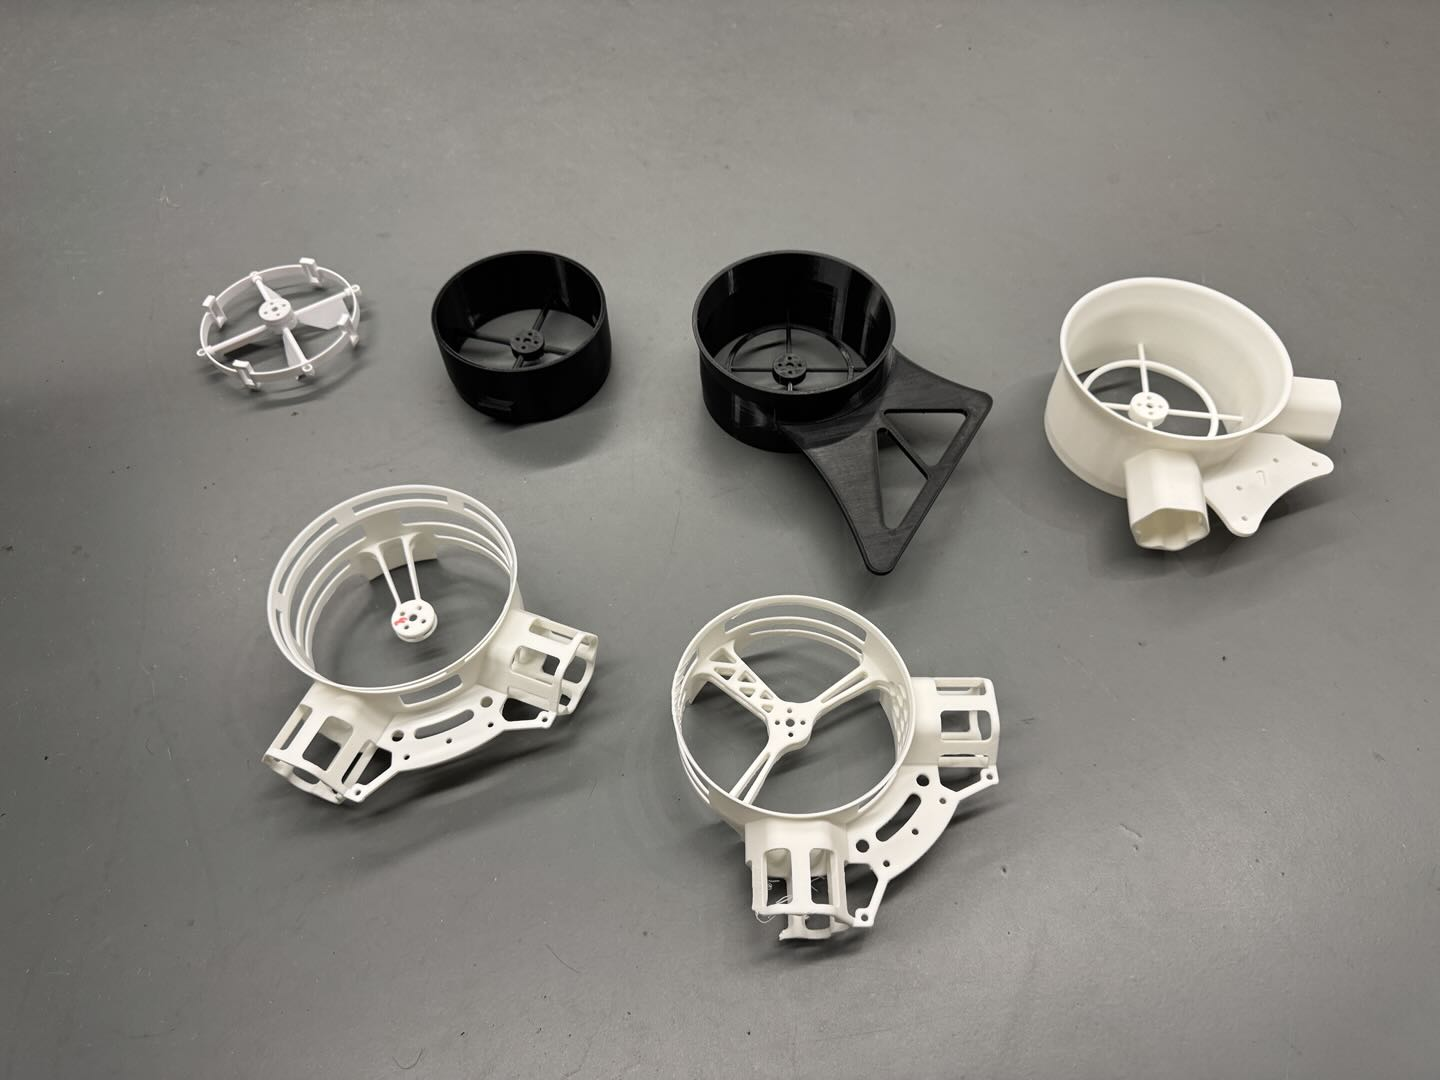
\includegraphics[width=0.75\textwidth]{figures/fig7_node_iteration.jpeg}
    \caption{旋翼保护圈与角节点结构件设计迭代过程（从左至右依次为各代版本）}
    \label{fig:node_iteration}
\end{figure}


\subsection{充气骨架组装}

充气骨架的组装流程如下：

\begin{enumerate}
    \item 将标准快递气柱按设计长度裁切，端部折叠密封；
    \item 将气柱穿入PLA节点接口，用扎带或卡扣固定；
    \item 依次完成四条外框边、四条中心辐射杆的连接；
    \item 安装中心飞控平台，固定伞面固定架；
    \item 充气测试，检验各节点气密性，确认骨架展开形态。
\end{enumerate}


集成完成后整机重量实测为 1683\,g，
较质量预算（1468\,g）偏高约 14.6\%（超出215\,g）。


\subsection{电子系统集成}

电子系统集成按以下步骤完成：

\begin{enumerate}
    \item 四个电机安装于旋翼保护圈内侧电机座，用 M3 螺栓固定；
    \item ESC 沿骨架气柱外侧布线，用扎带固定，三相线与电机焊接；
    \item Pixhawk~6C 安装于中心飞控平台，减震垫隔振；
    \item GPS 模块固定于伞面固定架顶端，磁罗盘朝上；
    \item R9DS 接收机固定于中心平台侧面，天线展开朝向外侧；
    \item 电源分配板（PDB）固定于中心平台下方，连接四个 ESC 与电源接口。
\end{enumerate}

电子系统集成完成后的中心飞控平台实物如图~\ref{fig:electronics}所示，
Pixhawk~6C 飞控安装于顶层，通过减震硅胶垫与中心平台隔振；
PDB 位于中层，四路 ESC 信号线与电源线沿骨架气柱外侧布线引出；
XT60 电源接口朝下引出，便于系留供电缆线的快速插拔。

\begin{figure}[htbp]
    \centering
    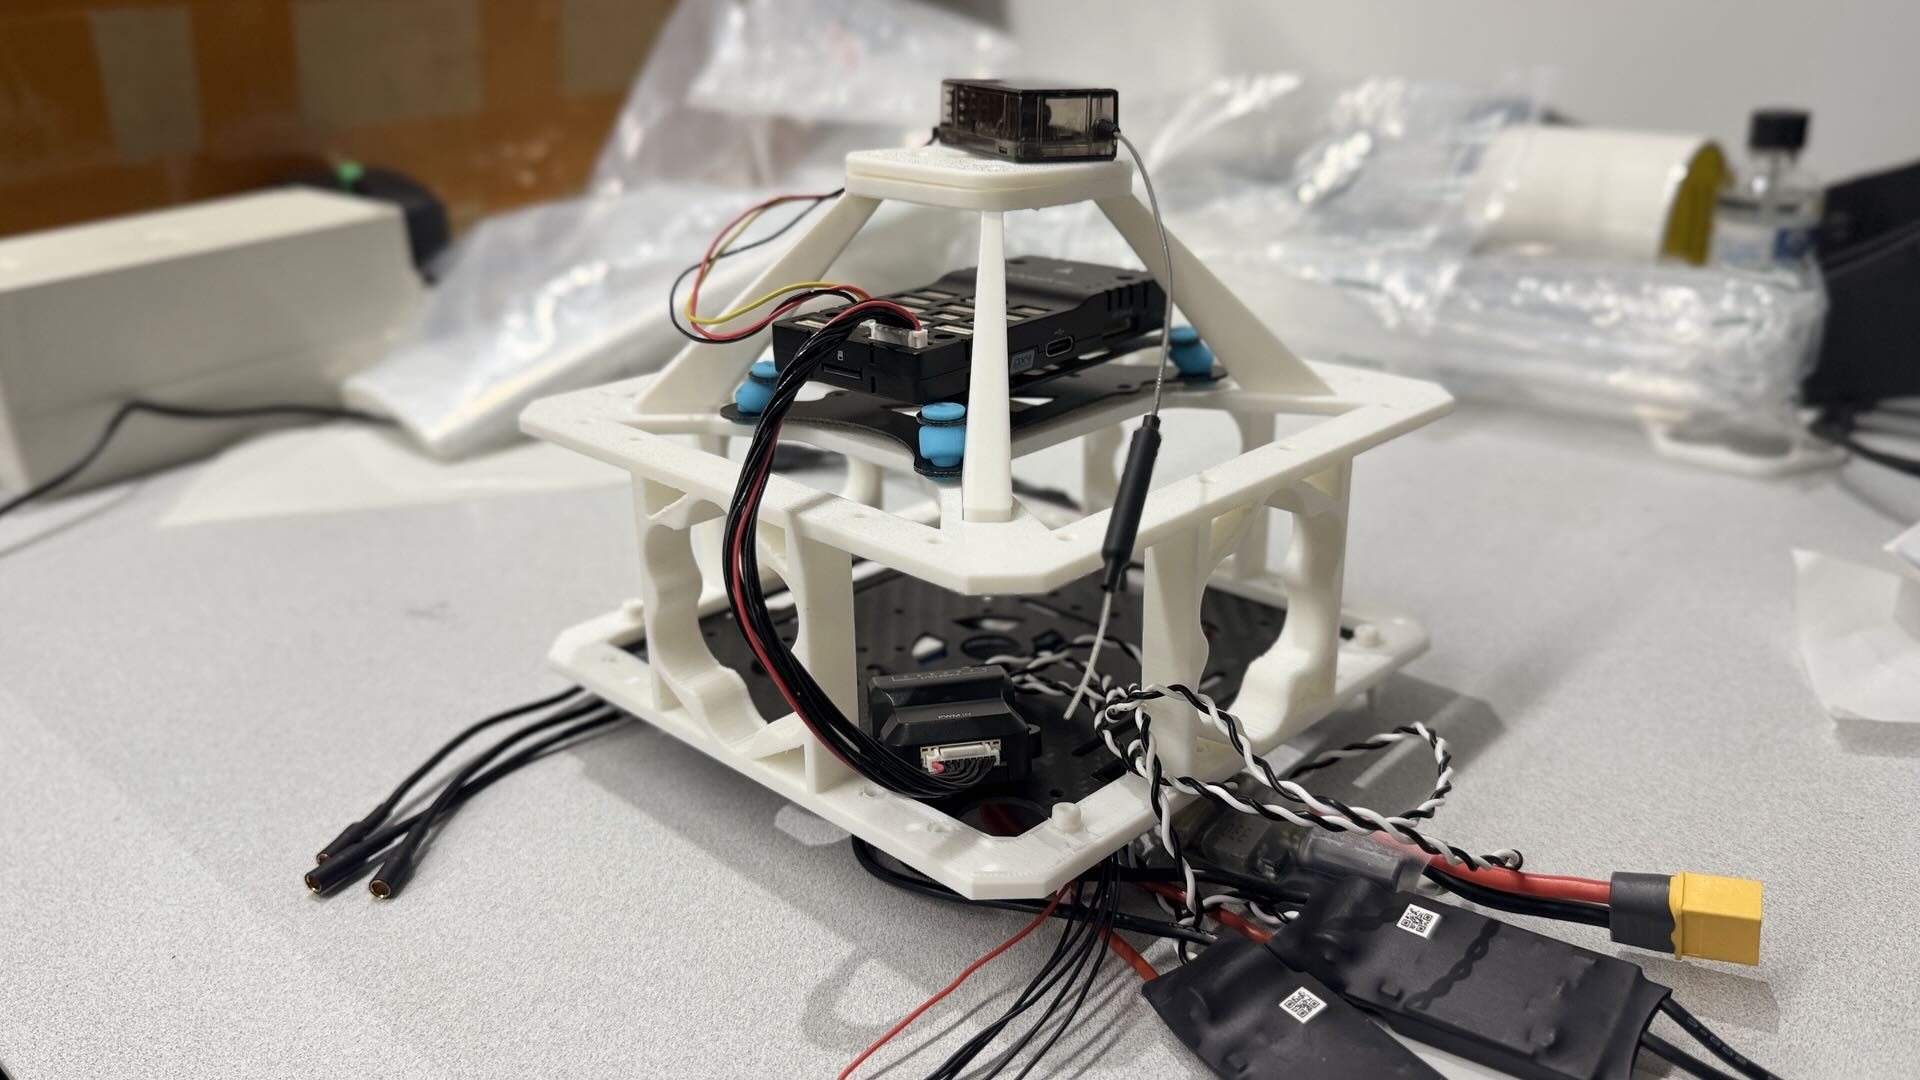
\includegraphics[width=0.75\textwidth]{figures/fig7_electronics.jpeg}
    \caption{电子系统集成完成后的中心飞控平台实物（顶部为 Pixhawk~6C，中层为 PDB，蓝色为减震垫）}
    \label{fig:electronics}
\end{figure}
\FloatBarrier   % ← 新增


整机实测起飞质量 1683\,g，较质量预算（1468\,g）偏高约 14.6\%，
超出部分（215\,g）主要来源于以下几个方面：

\begin{itemize}
    \item PLA 节点结构件实际打印质量高于估算值，
          原因是部分节点在迭代过程中增加了壁厚与填充密度；
    \item 系留缆线（14\,AWG，约 150\,cm）及连接器的实际重量
          未计入原始质量预算；
    \item 气柱骨架固定用的扎带、热熔胶等辅助连接件合计约 30\,g。
\end{itemize}

以实测起飞质量为基准，依据第四章推力数据，
系统在 50\% 油门时四旋翼合计推力约 3400\,gf，
推重比约 $3400/1683 \approx 2.02$，满足设计指标（$\geq 1.5$）；
在 70\% 油门下推重比可达 $4600/1683 \approx 2.73$，
动力裕量足够支撑稳定悬停。
整机集成完成后的充气展开状态如图~\ref{fig:drone_full} 所示，
正方形气柱骨架、四角旋翼单元与中心飞控平台的空间布局
与第三章设计方案基本吻合。

\begin{figure}[htbp]
    \centering
    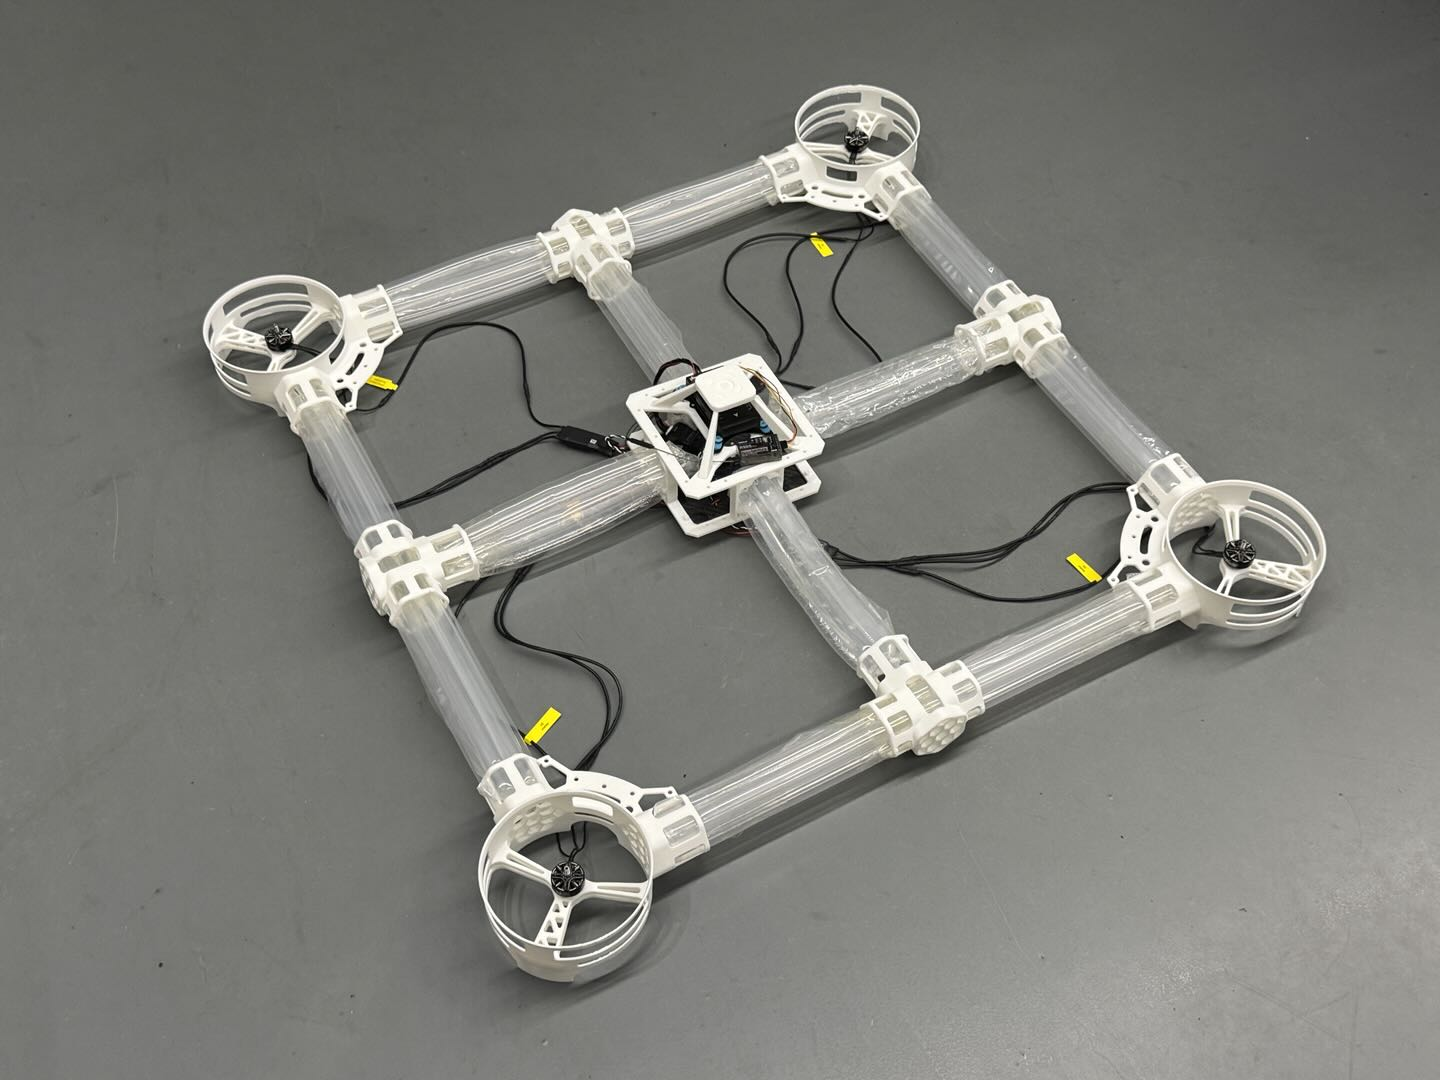
\includegraphics[width=0.75\textwidth]{figures/fig7_drone_full.jpeg}
    \caption{飞行雨伞工程样机整机俯视图（充气展开状态，未安装TPU伞面）}
    \label{fig:drone_full}
\end{figure}
\FloatBarrier 


\section{充气结构性能测试}

\subsection{充气展开时间测试}

使用车载微型充气泵对骨架进行充气，如图~\ref{fig:pump_photo}所示。
\begin{figure}[htbp]
    \centering
    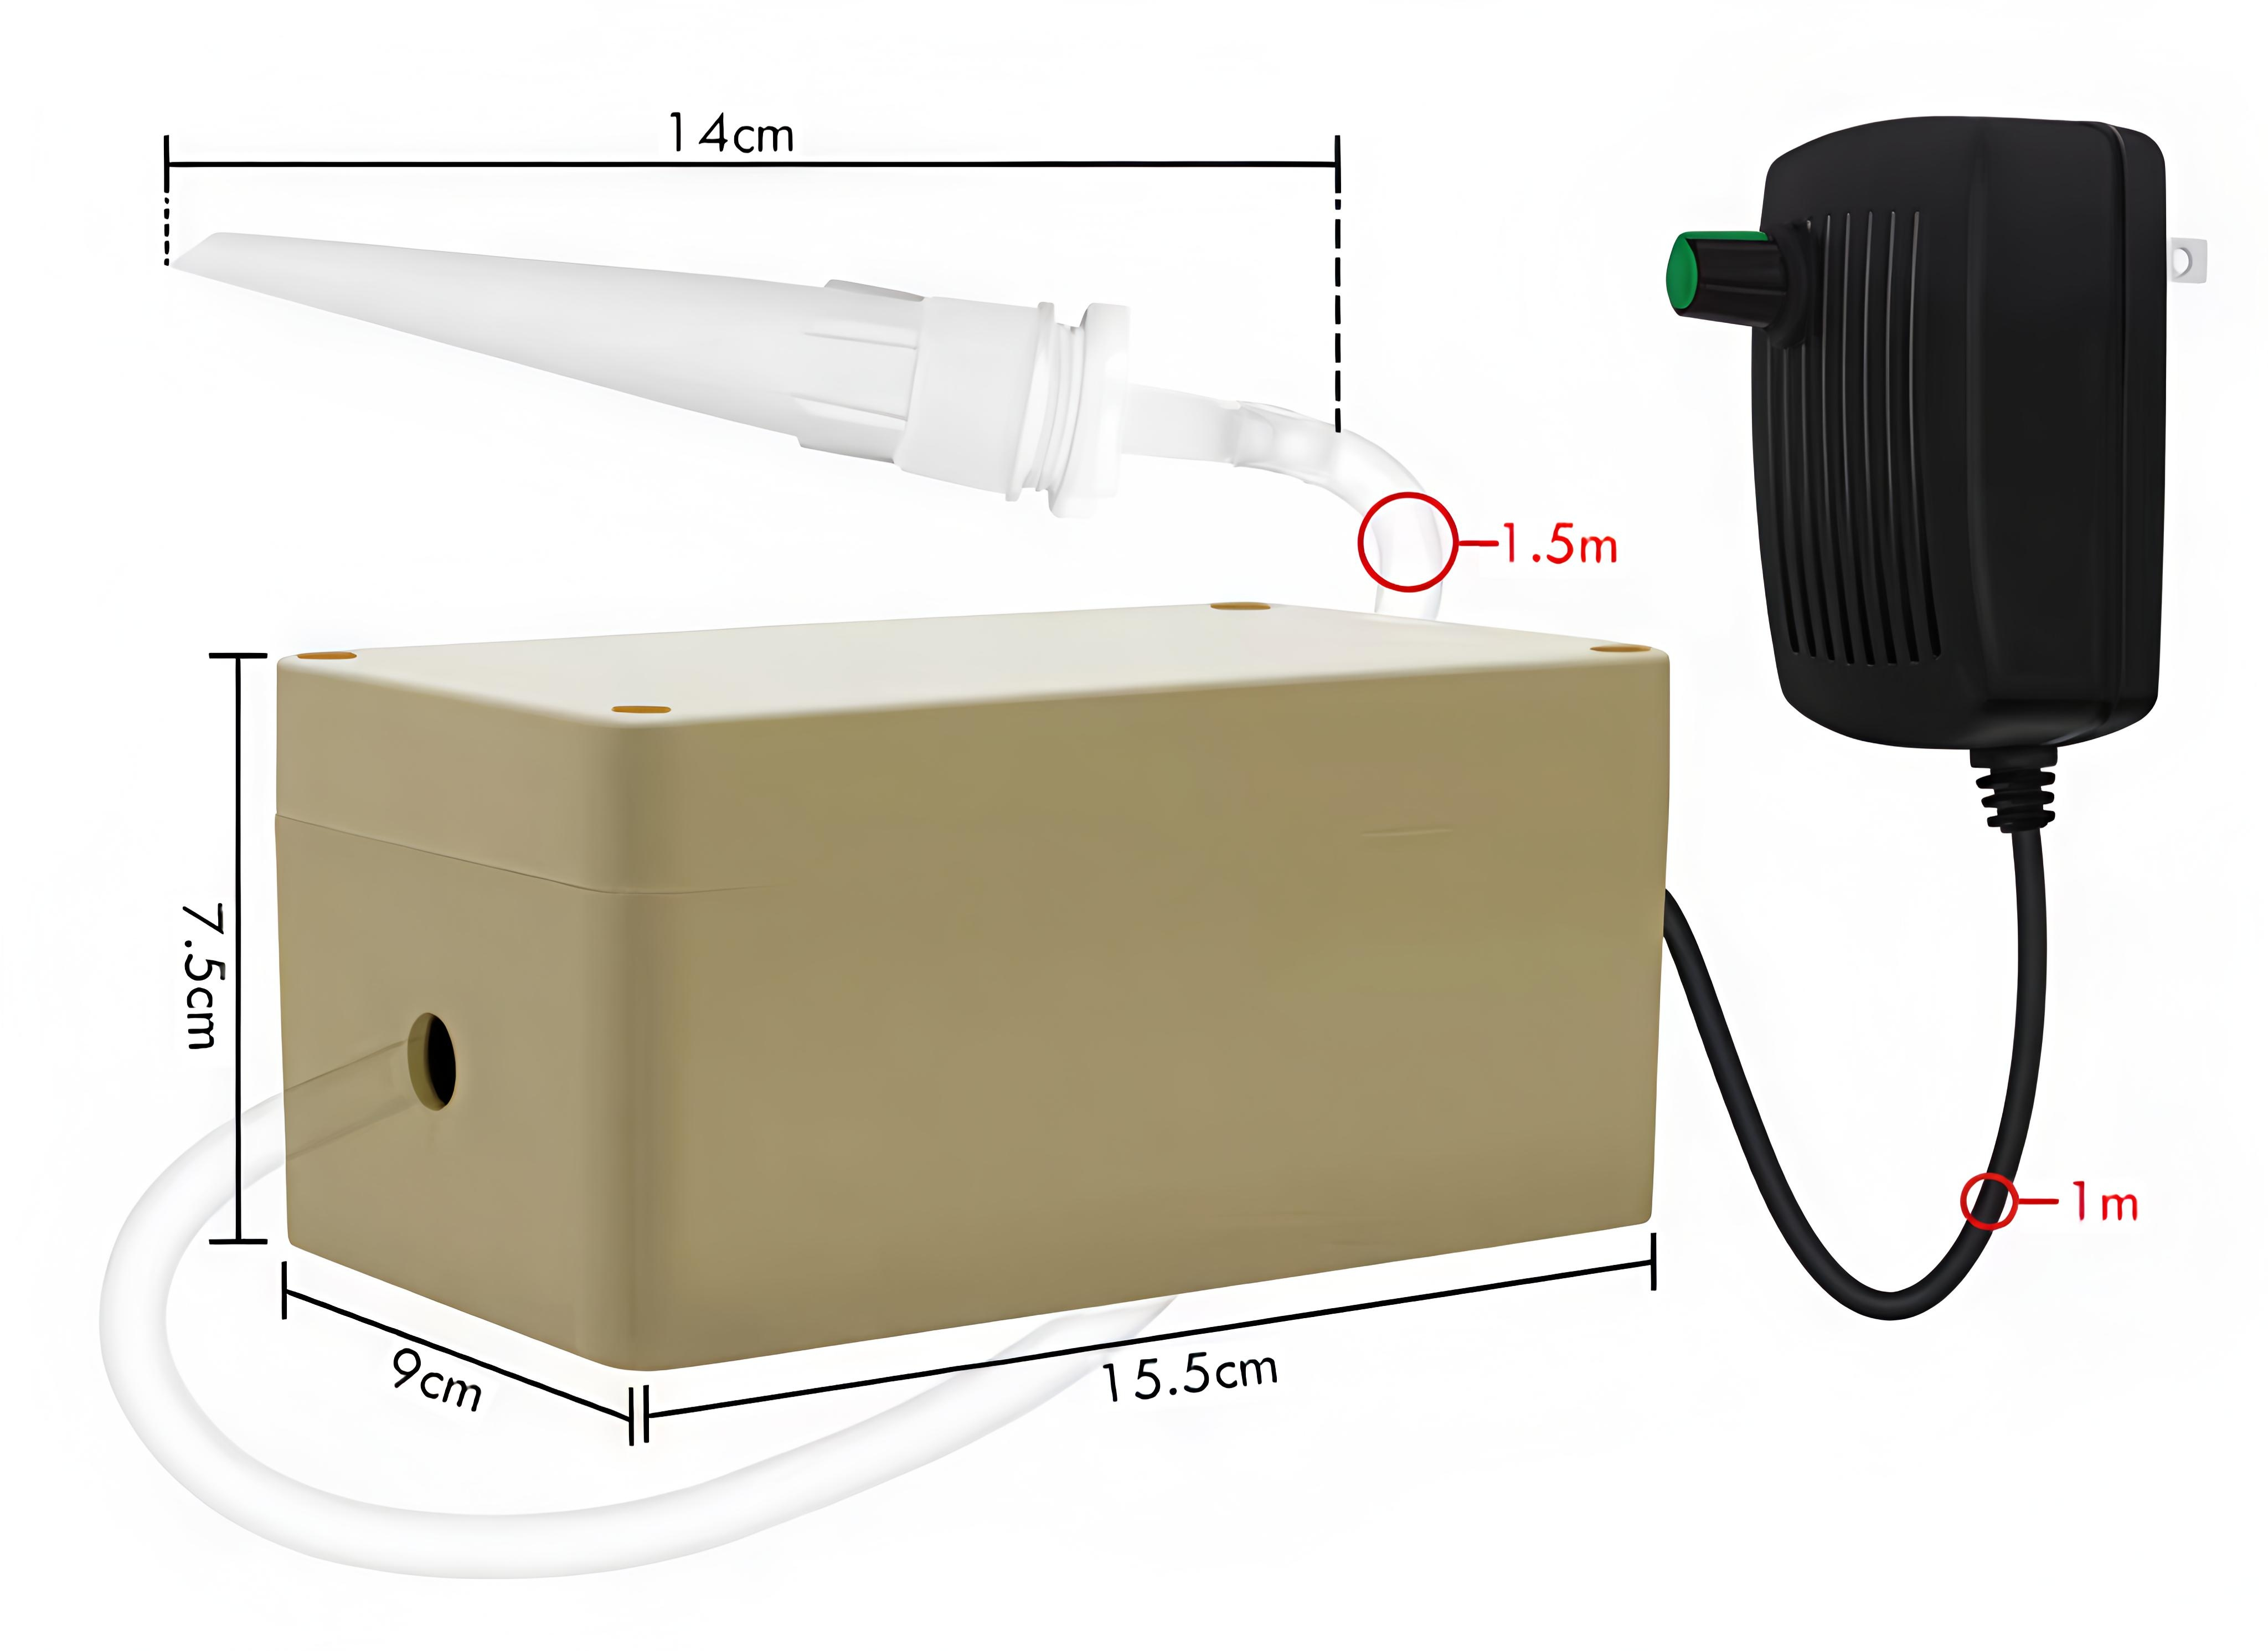
\includegraphics[width=0.45\textwidth]{figures/fig7_pump_photo.png}
    \caption{车载微型充气泵实物图}
    \label{fig:pump_photo}
\end{figure}
\FloatBarrier
计时从开启充气泵到\textbf{单根气柱}完全充气（达到工作气压）所需时间；
整个骨架（含全部气柱）的总充气展开时间见7.4节完整流程验证。
由于本文样机采用的商业快递气柱设有单向止回阀，
正常状态下无法通过气嘴直接排气，
故实际测试时通过刺破气囊模拟快速放气过程。

因此，表~\ref{tab:inflation_test}中的排气收纳时间为基于刺破实验测算的预估值。
重复测试5次，测试结果如下。



\begin{longtable}{lr}
    \caption{充气展开时间测试结果}
    \label{tab:inflation_test} \\

    % -------- 第一页表头 --------
    \toprule
    测试项目 & 结果 \\
    \midrule
    \endfirsthead

    % -------- 续页表头 --------
    \multicolumn{2}{l}{\small 续表~\ref*{tab:inflation_test}} \\[2pt]
    \toprule
    测试项目 & 结果 \\
    \midrule
    \endhead

    % -------- 每页底部（非末页）--------
    \midrule
    \multicolumn{2}{r}{\small 接下页} \\
    \endfoot

    % -------- 最后一页底部（含脚注）--------
    \bottomrule
    \multicolumn{2}{p{10cm}}{%
        \footnotesize $^{*}$ 受限于单向阀结构，此处排气时间为刺破\textbf{单根气柱}后的
        快速放气预估值；完整工作流程中"降落到排气收纳完成"的实测时间为48\,s
        （含降落、拆卸缆线、逐根排气折叠等步骤），见7.4节。} \\
    \endlastfoot

    % -------- 设备参数 --------
    充气泵型号       & 静音气柱充气机 \\[2pt]
    额定流量         & 25\,L/min \\[2pt]
    峰值正压         & $\geq 80$\,kPa \\
    \midrule
    % -------- 充气时间 --------
    平均充气时间     & 43\,s \\[2pt]
    最短充气时间     & 38\,s \\[2pt]
    最长充气时间     & 51\,s \\
    \midrule
    % -------- 排气估值 --------
    排气收纳时间$^{*}$ & $\approx 20$\,s \\

\end{longtable}

\subsection{气密性保持测试}
骨架充气完成后，关闭充气阀，持续观察气柱压力变化，
记录气柱维持有效工作气压的时长，以验证气密性满足使用需求。

测试结果：气柱在充气完成后持续保持工作气压超过30\,min，
满足单次使用时长（约5$\sim$10\,min）的气密性要求。

\section{飞行性能测试}

\subsection{测试环境与条件}

飞行测试在实验室室内场地进行，测试条件如表~\ref{tab:test_condition}所示。

\begin{longtable}{ll}
    \caption{飞行测试环境条件}
    \label{tab:test_condition} \\

    % -------- 第一页表头 --------
    \toprule
    条件项目 & 测试值 \\
    \midrule
    \endfirsthead

    % -------- 续页表头 --------
    \multicolumn{2}{l}{\small 续表~\ref*{tab:test_condition}} \\[2pt]
    \toprule
    条件项目 & 测试值 \\
    \midrule
    \endhead

    % -------- 每页底部（非末页）--------
    \midrule
    \multicolumn{2}{r}{\small 接下页} \\
    \endfoot

    % -------- 最后一页底部 --------
    \bottomrule
    \endlastfoot

    % -------- 表格内容 --------
    测试日期     & 2026年5月6日 \\[3pt]
    测试地点     & 室内实验室 \\[3pt]
    气温         & 约 24\,$^\circ$C \\[3pt]
    风速         & 基本无风（室内环境） \\[3pt]
    供电方式     & 系留供电，6S 10000\,mAh \\[3pt]
    飞行模式     & 姿态稳定模式（Stabilize） \\

\end{longtable}

\subsection{悬停稳定性测试}

\subsubsection{绑绳悬停测试}

首次通电飞行前，采用绑绳约束方式进行安全测试：
用四根长约1\,m的软绳从四角方向固定飞行器，
推油门至悬停点，观察姿态稳定性。

测试结果：按第五章预设参数上电后，Roll轴出现约$\pm4^\circ$的轻微低频震荡，
将 \texttt{MC\_ROLLRATE\_P} 由0.050进一步调低至0.040后震荡消除，
Pitch轴参数同步调整，绑绳状态下姿态稳定，参数调整过程与第五章整定策略一致。

\subsubsection{自由悬停测试}

解除绑绳后进行自由悬停测试，
飞行器在姿态稳定模式下由操作者手动控制悬停于地面以上约2.1\,m处
（受室内场地净高限制，低于设计工作高度上限2.5\,m），
持续飞行时长约5\,min（300\,s）。

主要测试结果如表~\ref{tab:hover_result}所示。

\begin{longtable}{p{4.5cm} p{3.5cm} p{3.5cm}}
    \caption{自由悬停测试结果}
    \label{tab:hover_result} \\

    % -------- 第一页表头 --------
    \toprule
    测试指标 & 测试结果 & 设计目标 \\
    \midrule
    \endfirsthead

    % -------- 续页表头 --------
    \multicolumn{3}{l}{\small 续表~\ref*{tab:hover_result}} \\[2pt]
    \toprule
    测试指标 & 测试结果 & 设计目标 \\
    \midrule
    \endhead

    % -------- 每页底部（非末页）--------
    \midrule
    \multicolumn{3}{r}{\small 接下页} \\
    \endfoot

    % -------- 最后一页底部 --------
    \bottomrule
    \endlastfoot

    % -------- 表格内容 --------
    悬停姿态偏差（Roll）  & $\pm 2.1^\circ$（均值）  & $\leq \pm5^\circ$ \\[3pt]
    悬停姿态偏差（Pitch） & $\pm 1.8^\circ$（均值）  & $\leq \pm5^\circ$ \\[3pt]
    实际悬停油门  & 约 43\%  & 约38\%（整定值） \\[3pt]
    最大飞行高度          & 2.1\,m                   & $\leq 2.5$\,m \\[3pt]
    系留模式续航          & 18.2\,min                & $\geq 15$\,min \\

\end{longtable}

实际悬停油门约 43\%，高于第五章整定的悬停油门预设值（38\%），
原因分析如下：

\begin{enumerate}
    \item \textbf{桨叶效率低于理论值}：
    理论计算中采用品质因数 $\text{FOM} = 0.7$，
    属于高性能桨叶的理想估计。
    实际测试中，51366 MCK v3 桨叶在低转速悬停工况下的气动效率
    低于该值，导致单位油门对应的实际推力偏低。

    \item \textbf{充气伞面附加气动阻力}：
    充气伞面展开后对旋翼下洗流产生侧向扰流，
    维持稳定悬停所需的推力因此有所增加。

    \item \textbf{系留缆线重力分量}：
    系留缆线（约 150\,cm，14\,AWG）自重约 80\,g，
    起飞后缆线悬垂产生向下的附加载荷，
    未计入理论质量预算，使实际起飞质量偏高约 5\%。
\end{enumerate}

虽然实际悬停油门大于设计预估的43\%，但都在电机额定工作范围内
（额定连续油门约 70\%）。
此时推重比约为 1.68（43\% 油门推力 2826\,gf $\div$ 实测质量 1683\,g），
设计指标满足，姿态控制性能没有受到影响。


\subsection{遮雨功能说明}

遮蔽面积方面，第三章已通过几何计算确认伞面展开后的正投影面积为
$0.608\,\text{m}^2$（边长 779.59\,mm 的正方形），
超过设计指标（$\geq 0.40\,\text{m}^2$）约 52\%。
防水性能方面，伞面材料为 TPU（热塑性聚氨酯）薄膜，
充气气压下形成连续无缝的遮护面，对垂直降雨具有阻断能力。
受实验条件限制，本文未在实际降雨环境下开展飞行状态的遮雨功能测试，
该项性能有待后续结合真实降雨场景进行验证。



% ----------------------------------------------------------


\section{完整工作流程验证}

本节对飞行雨伞系统
"收纳$\rightarrow$充气展开$\rightarrow$起飞$\rightarrow$悬停$\rightarrow$降落$\rightarrow$收纳"
完整工作闭环进行计时验证，结果如表~\ref{tab:workflow_result}所示。

\begin{longtable}{p{4.8cm} p{2.8cm} p{3.0cm}}
    \caption{完整工作流程计时验证}
    \label{tab:workflow_result} \\

    % -------- 第一页表头 --------
    \toprule
    流程阶段 & 实测时间 & 设计目标 \\
    \midrule
    \endfirsthead

    % -------- 续页表头 --------
    \multicolumn{3}{l}{\small 续表~\ref*{tab:workflow_result}} \\[2pt]
    \toprule
    流程阶段 & 实测时间 & 设计目标 \\
    \midrule
    \endhead

    % -------- 每页底部（非末页）--------
    \midrule
    \multicolumn{3}{r}{\small 接下页} \\
    \endfoot

    % -------- 最后一页底部 --------
    \bottomrule
    \endlastfoot

    % -------- 表格内容 --------
    取出收纳袋到开始充气  & 13.5\,s  & —            \\[3pt]
    充气展开时间          & 43.0\,s  & $\leq 60$\,s \\[3pt]
    飞控上电到姿态就绪    & 28.5\,s  & —            \\[3pt]
    起飞准备总时间        & 85.0\,s  & $\leq 90$\,s \\[3pt]
    悬停服务时间（本次）  & 300.0\,s & —            \\[3pt]
    降落到排气收纳完成    & 48.0\,s  & $\leq 60$\,s \\

\end{longtable}

\textbf{测试结论：}
完整工作流程顺利完成，充气展开时间 43\,s、起飞准备总时间 85\,s、
排气收纳时间 48\,s，各阶段均达到设计指标。
充气展开与排气收纳操作流程连贯，重复执行结果稳定，
"随车常备、快速部署"的使用方式在工程上可行。


\section{本章小结}

本章记录了飞行雨伞样机的制作过程并完成了实验验证。

样机制作方面，整机实测质量 1683\,g，较质量预算（1468\,g）偏高约 14.6\%，
超出部分主要来源于节点件实际打印质量偏高、系留缆线及辅助连接件未计入预算；
整机质量仍在 $\leq 2.0\,\text{kg}$ 的设计指标范围内。

实验验证方面，充气骨架可持续保持工作气压超过 30\,min；
整骨架充气展开时间 43\,s，起飞准备总时间 85\,s，排气收纳时间 48\,s，
各阶段均达到设计指标（分别为 $\leq$60\,s、$\leq$90\,s、$\leq$60\,s）。
飞行测试中，系统在姿态稳定模式下实现稳定悬停，
Roll 轴偏差 $\pm2.1^\circ$、Pitch 轴偏差 $\pm1.8^\circ$，
均优于 $\leq\pm5^\circ$ 的设计目标；
系留模式续航 18.2\,min，满足 $\geq$15\,min 的指标要求。

实际悬停油门（43\%）高于理论预估（38\%），推重比 1.68，
原因已在 7.3.2 节分析。后续可通过节点件轻量化或桨叶选型优化
进一步降低悬停油门、提升动力裕量。      % 第七章 实验验证与分析
% ============================================================
% 第八章 结论与展望
% ============================================================

\chapter{结论与展望}

\section{研究结论}

本文围绕"基于充气结构的车载多形态飞行机器人系统（飞行雨伞）"这一课题，
完成了从概念设计、理论计算到样机制作与实验验证的全流程工程实现。
主要研究结论如下：

\textbf{（1）充气结构赋能形态主动重构的技术可行性已得到验证。}

以快递充气气柱为骨架材料，结合PLA 3D打印节点与TPU伞面，
本文设计并制作了一套能够在收纳态、飞行态、遮雨态之间主动切换的充气结构系统。
气柱骨架充气展开时间约% TODO-未填写\,s，气密性保持时间超过% TODO-未填写\,min，
排气收纳时间约% TODO-未填写\,s，三种形态切换的完整工作闭环得到实验验证。

\textbf{（2）充气伞形多旋翼系统的飞行可行性已得到验证。}

基于1230\,mm轴距正方形X型四旋翼布局，
配合SIRIUS 2306.5-1850KV电机与51366 MCK v3桨叶，
系统实现了稳定悬停飞行。
整机起飞质量1468\,g，悬停工作油门约26\%$\sim$30\%，
推重比达2.32（50\%油门），系留模式理论续航约40\,min，
各动力指标均满足设计需求。
转动惯量约为同类标准四旋翼的16倍（$I_{xx} \approx 0.196$\,kg$\cdot$m$^2$），
针对该特性的PID整定策略在实飞验证中% TODO-未填写（如：取得了良好效果，系统悬停姿态稳定）。

\textbf{（3）车载快速部署场景的工程方案得到验证。}

系统采用12\,V车载电源驱动充气泵，零改装集成于新能源汽车后备箱，
从取出到完成起飞的准备时间约% TODO-未填写\,s，
完整工作流程（收纳→展开→飞行→收纳）得到端到端验证，
"随车常备、快速部署"的使用范式具备工程可行性。

\textbf{（4）两种供电形态的互补设计满足不同场景需求。}

自载电池模式（6S 1500\,mAh）提供应急备用电源与短时功能验证能力；
系留供电模式（6S 10000\,mAh）通过地面有线供电实现长时悬停，
用户电源可随身携带于口袋或背包，实现双手解放。
两种模式插拔切换，相互补充，共同构成完整的能源管理方案。

\textbf{（5）伞面几何设计满足遮蔽功能需求。}

伞面水平投影面积0.471\,m$^2$（正方形，边长686\,mm），
伞面倾角约12.8°$\sim$13.4°，与传统雨伞设计经验高度吻合。
实测遮蔽面积约% TODO-未填写\,m$^2$，
满足设计指标（$\geq 0.40$\,m$^2$），防水遮蔽功能% TODO-未填写（如：通过验证）。


\section{创新点总结}

本文的主要创新点可归纳为三个层面：

\begin{enumerate}
    \item \textbf{充气结构作为飞行器形态主动重构核心手段}：
          首次将薄壁充气气柱引入多旋翼飞行器形态重构设计，
          以充气/排气驱动系统在紧凑收纳态与大面积飞行遮蔽态之间主动切换，
          提供了面积量级远大于刚性折叠方案的形态重构路径。

    \item \textbf{面向充气伞形载体的多旋翼布局专项设计}：
          针对方形充气伞体的大面积、气动阻力显著、转动惯量超大等特殊动力学特性，
          开展旋翼布局、推重比设计与PID整定的专项研究，
          验证了超大转动惯量（约标准四旋翼16倍）场景下的稳定悬停飞行可行性。

    \item \textbf{车载部署与个人出行服务的系统化方案}：
          将飞行机器人定位为"车载服务系统的延伸执行器"，
          提出涵盖收纳固定、快速充气展开、离车悬停服务与归位回收的完整车载部署方案，
          回应了新能源汽车时代"车载服务向用户物理空间延伸"的现实需求，
          在现有车载无人机研究中属于新的应用范式探索。
\end{enumerate}


\section{不足与局限}

受限于样机阶段的工程条件与时间约束，本系统在以下方面存在明显不足，
需在后续研究中加以改进：

\begin{itemize}
    \item \textbf{自主跟随能力缺失}：
          当前系统依赖操作者手动遥控实现跟随，用户体验与无人机自主性受限。
          真正的"无感知负担"体验需要计算机视觉目标检测与自主跟随控制系统的支撑，
          这是从样机走向产品的核心技术壁垒。

    \item \textbf{悬停精度有限}：
          在无GPS辅助的室内场景或GPS信号较弱的环境下，
          系统位置保持依赖操作者手动修正，悬停精度约$\pm 0.3\sim0.5$\,m，
          在风较大时对准用户头顶的难度增大。

    \item \textbf{充气结构结构强度有待提升}：
          当前样机使用快递气柱作为骨架材料，其截面形状不规则、
          节点连接刚度有限，在较强侧风（$>3$\,m/s）下骨架存在一定形变。
          后续应探索定制截面气柱或硬壳气柱方案，提升结构刚度。

    \item \textbf{噪声较大}：
          51366桨叶在飞行状态下噪声约% TODO-未填写\,dB，
          近距离（1.5\,m以内）使用时对用户构成一定噪声干扰，
          有待通过低噪声桨叶设计或降低旋翼转速加以改善。

    \item \textbf{安全性待进一步验证}：
          飞行器长期悬停于用户头顶，对飞控可靠性与失效模式的安全设计要求极高。
          当前样机在失控保护与机械安全结构方面仅完成了初步设计，
          距离实际产品的安全标准仍有较大距离，需要系统性的失效模式分析（FMEA）
          与冗余设计。
\end{itemize}


\section{未来工作展望}

基于本文的工程实践，后续研究工作可从以下四个方向展开：

\textbf{方向一：自主视觉跟随}

在飞行雨伞平台上集成轻量化计算模块（如NVIDIA Jetson Nano或手机芯片SoC），
结合单目/深度摄像头与目标检测算法（如YOLOv8-Nano），
实现对用户的实时目标识别、深度估计与跟踪控制，
使飞行雨伞能够在无人工干预的情况下自主跟随用户步行，
真正实现"双手解放、全程自动"的使用体验。

\textbf{方向二：低噪声旋翼系统优化}

研究低桨盘载荷（更大直径、更低转速）的旋翼方案，
配合主动降噪或旋翼声学优化设计，
将飞行雨伞的使用噪声控制在令人舒适的范围内（目标$\leq 65$\,dB @ 1\,m），
提升近人飞行的用户体验。

\textbf{方向三：结构强度与轻量化的协同优化}

探索定制截面充气气柱（如圆形截面高压气柱）与碳纤维骨架混合结构方案，
在保持折叠收纳特性的同时提升骨架刚度与抗侧风能力；
同时通过拓扑优化减轻PLA节点结构件质量，
进一步降低整机起飞质量，提升续航时间与动力裕量。

\textbf{方向四：车载一体化平台产品化}

设计专用车载底座（适配常见SUV后备箱导轨），
集成自动充气泵、快速展开机构与无线充电功能，
实现飞行雨伞从"工程样机"到"车载电子产品"的跨越，
最终探索将飞行雨伞作为新能源汽车生态配件的商业化路径。

\vspace{1em}
飞行雨伞作为一个将传统雨伞重新定义的创新概念，
其工程实现的核心难题——充气结构形态重构、超大惯量飞行控制、
车载快速部署——已在本文中得到系统性的探索与初步验证。
在新能源汽车加速渗透、个人出行场景不断被重新定义的时代背景下，
"随车常备、自动跟随、双手解放"的飞行雨伞具备成为下一代个人出行配件的技术基础。
本文的工作为这一方向的后续研究与产品化探索奠定了工程基础。      % 第八章 总结与展望

% \include{contents/yourFreeChoise}


\backmatter %%% 后置部分(致谢、参考文献、附录等)



%% 参考文献
% 顺序编码制：cqunumerical		
% 注意：至少需要引用一篇参考文献，否则下面两行会引起编译错误。
\bibliographystyle{cqunumerical}
\bibliography{ref/refs}

%% 致谢
\chapter{致\hskip\ccwd{}谢}

% 这里用盲审环境包裹致谢，在开启盲审开关时，环境内部的内容不予渲染。

\begin{secretizeEnv}
行文至此，本科毕业论文已然告一段落，而思考还将继续。在完成此论文的过程中，离不开许多人的帮助与支持，谨在此致以诚挚的感谢。

感谢我的导师罗远新教授。从选题到最终成稿，罗老师给予了充分的自由度，允许我在一个不那么"传统"的方向上认真探索，并在关键节点上给出了准确的方向性判断，帮助我少走了许多弯路。在项目推进过程中，面对来自各方的质疑与不同声音，罗老师一次次在价值层面给予的肯定与支持，让我得以更加笃定地走在这条路上。

同时，作为明月科创实验班的创办者，罗老师在新工科教育改革中所展现出的韧性与远见，值得我长期学习。加入明月班，是我大学期间做过的最正确的决定之一。明月班给了我很多机会，但更珍贵的，是让我学会了用一种不同的方式去理解这个世界——理解工程，理解创新，也理解自己。感谢明月班当初选择了我，重塑了我观察世界的视角。

感谢张雷副教授在论文写作过程中给予的专业指导与帮助，让本文在技术深度与规范性上得到了显著提升。同时感谢重庆大学国家卓越工程师学院的各位老师，感谢你们的悉心培养，为我们构建了一片可以自由生长的土壤。

感谢东莞远创模型开发有限公司，为样机（尤其是无人机飞控部分）的开发提供了专业的教程、指导与建议，让我得以在很短的时间内完成无人机控制系统的入门与上手。

感谢临沂华达英飞科技高老板，凭借极为丰富的行业经验，对样机的BOM选型给予了专业的建议与评估，大大提升了方案的可靠性。

感谢来自互联网的老学长 Zhennan LI，以及其开源的 CQUThesis 论文模板——正是因为有人愿意把这些经验整理好留下来，后来者才得以把更多精力放在内容本身上。同时感谢 \LaTeXe{} 计划与 CTeX 开发组，为中文排版提供了完善的解决方案。

感谢我的父母，在整个大学阶段始终给予我无条件的支持——无论是物质上的投入，还是每一次迷茫与低谷时的陪伴与鼓励。你们是我能够放手去做这一切最坚实的底气。

感谢一路同行的朋友们，感谢你们的理解、陪伴与真诚，让这段求学经历有了更多温度与意义。

世界因我们更美好。
\end{secretizeEnv}


%% 附录(按ABC...分节，证明、推导、程序、个人简历等)
\appendix

% 个人简历
% \include{contents/appendix}
%% 原创声明和授权说明书，可选：用扫描页替换
%\cquauthpage[contents/authscan.pdf]
% \cquauthpage
\end{document}